\documentclass{tubaf-report}
\usepackage[sans]{tubaf-fonts}
\usepackage[english]{babel}

\usepackage[T1]{fontenc}
\usepackage[utf8]{inputenc}

\usepackage{graphicx}
\usepackage{amsmath}
\usepackage{amssymb}
\usepackage{tabularx}
\usepackage{array}
\usepackage{booktabs}
\usepackage{multirow}
\usepackage{tikz}
\usepackage{float}
\usepackage{fvextra}
\usepackage{microtype}
\usepackage{capt-of}
\usetikzlibrary{arrows.meta,positioning,shapes.geometric}

\usepackage[numbers,sort&compress]{natbib}
\usepackage{url}
\usepackage[hidelinks]{hyperref}

\setcounter{tocdepth}{2}
\setcounter{secnumdepth}{3}

\newcommand{\refnote}[1]{\textbf{[REF: #1]}}

\begin{document}

\title{Implementation of a Simulation Tool for the Gray--Scott Model}
\subtitle{}
\author{Mehdi Bakhshi Zadeh}
\date{5 April 2026}
\subject{Personal Programming Project}
\publishers{%
Computational Materials Science\\
Fakult\"at IV\\[1.5em]
Matriculation Number: 69524\\[1.5em]
Supervised by\\
Dr.\ rer.\ nat.\ habil.\ Uwe Pr\"ufert\\[1.5em]
Professor In Charge \\
Prof.\ Dr.-Ing.\ habil.\ Bernhard Eidel\\
Dr.-Ing.\ habil.\ Arun Prakash\\
Dr.-Ing.\ Stefan Pr\"uger
}

\maketitle

\pagenumbering{roman}

% Prevent blank right-hand pages in front matter
\let\cleardoublepage\clearpage

\tableofcontents
\listoffigures
\listoftables

\chapter*{Abstract}
\addcontentsline{toc}{chapter}{Abstract}

This project presents the development of a MATLAB simulation tool for the two-dimensional Gray--Scott reaction--diffusion model. The final program combines a shared numerical core with both non-GUI and GUI-based workflows, and includes multiple diffusion implementations, configurable boundary conditions, plotting and export utilities, reproducible verification tests, and benchmark scripts. The software was designed not only to produce Gray--Scott patterns, but also to provide a structured framework for testing solver correctness, comparing implementation variants, and supporting interactive exploration through an App Designer interface.

The numerical verification showed that the implementation reproduces the expected behavior of the underlying discretization methods. In particular, the manufactured-solution test confirmed second-order spatial accuracy of the discrete Laplacian, while the time-step study showed the expected first-order behavior of the explicit Euler scheme. Additional tests verified correct boundary-condition treatment, machine-precision agreement between matrix-based and stencil-based diffusion realizations, and consistency between GUI and non-GUI execution for the documented reference case. A Pearson-type pattern sanity check further supported the physical plausibility of the computed results.

A central practical objective of the project was to determine the most suitable solver configuration for the final implementation. The benchmark study showed that the dense formulation is mainly useful as a small-scale reference, whereas the sparse-matrix and stencil-based solvers are the practically relevant options. Among them, the stencil implementation showed the more favorable memory usage and scaling behavior over the relevant grid range, while remaining competitive in runtime. For this reason, the stencil solver was selected as the default solver in the final program. Overall, the project achieved its goal by delivering a verified, benchmarked, and usable Gray--Scott simulation tool with a modular structure suitable for further extensions.
\clearpage

\pagenumbering{arabic}

\chapter{Introduction}

\section{Motivation}

Although the Gray--Scott model is compact in mathematical form, its numerical simulation becomes computationally demanding when spatial and temporal resolutions are increased in order to resolve pattern formation accurately. In particular, explicit time integration imposes a restrictive stability condition that links the admissible time step size to the spatial mesh width. As the grid is refined, the number of required time steps rises rapidly, which makes the model a useful test problem not only for reaction--diffusion dynamics, but also for the practical assessment of numerical efficiency \refnote{Gray--Scott references}.

A further motivation of this work is that the diffusion term can be implemented in more than one numerically equivalent way. On a structured Cartesian grid, the discrete Laplacian has a highly regular stencil structure. It can be realized explicitly through a sparse matrix construction, but it can also be applied in stencil form without assembling the full operator. This creates a natural computational question: which implementation is the more suitable practical solver for the Gray--Scott problem in the present MATLAB framework?

\section{Objective}

The objective of this project is to implement a MATLAB-based simulation tool for the two-dimensional Gray--Scott model and to determine, through systematic verification and benchmarking, which solver approach is the best practical choice for the underlying partial differential equation. The work therefore combines model implementation, numerical testing, and performance comparison in a single software framework.

A central requirement is that solver evaluation must be based on correctness first and efficiency second. For this reason, the project does not rely only on visually plausible solutions or isolated timing measurements. Instead, the implemented methods are verified for consistency and correctness before they are compared with respect to runtime and memory usage. The final aim is thus to provide a dependable simulation tool whose recommended default solver is justified by evidence rather than by assumption.
\chapter{Theory and Mathematical Model}

\section{Gray--Scott reaction--diffusion system}

Reaction--diffusion systems describe processes in which chemical species both react locally and spread in space by diffusion. Even relatively simple nonlinear interactions can generate complex spatial structures such as spots, stripes, travelling fronts, and labyrinth-like patterns. For this reason, reaction--diffusion equations are widely used as model systems for studying self-organization and pattern formation in chemistry, physics, and biology \citep{gandy2022,pearson1993}.

The Gray--Scott model is a particularly well-known two-species reaction--diffusion system. It is based on an autocatalytic chemical mechanism in an open environment, where one component is continuously supplied and another is removed or decays. This continuous feeding and removal keep the system away from thermodynamic equilibrium and allow the formation of sustained non-uniform spatial patterns instead of simple relaxation to a homogeneous steady state \citep{gray1984,gandy2022,pearson1993}.

In its standard form, the model uses two scalar concentration fields, denoted here by $u(\mathbf{x},t)$ and $v(\mathbf{x},t)$. Their dynamics are governed by the interaction of local nonlinear reaction kinetics and spatial diffusion. The central mechanism is cubic autocatalysis, meaning that the presence of one species promotes further production of itself through reaction with the other species. At the same time, diffusion tends to smooth spatial gradients. The patterns observed in the Gray--Scott system therefore arise from the competition between local nonlinear amplification and spatial spreading.

The Gray--Scott model is especially suitable for the present project because it combines a compact mathematical structure with rich qualitative behaviour. Small changes in the model parameters can lead to significantly different dynamical regimes, which makes the system an effective benchmark for the study of pattern-forming partial differential equations and their numerical simulation \citep{gandy2022,pearson1993}.

\section{Interpretation of the model terms}

In the present work, the Gray--Scott model is written in the standard dimensionless form. Accordingly, the variables and parameters are treated here in nondimensional form, so explicit physical units are not attached in this report.
\begin{align}
\frac{\partial u}{\partial t} &= D_u \nabla^2 u - u v^2 + F(1-u), \label{eq:gs_u} \\
\frac{\partial v}{\partial t} &= D_v \nabla^2 v + u v^2 - (F+k)v . \label{eq:gs_v}
\end{align}
where $u(\mathbf{x},t)$ and $v(\mathbf{x},t)$ denote the concentrations of the two interacting species, $D_u$ and $D_v$ are their diffusion coefficients, $F$ is the feed rate, and $k$ is the removal or decay rate of the second species \citep{gandy2022,pearson1993}.

The diffusion terms, $D_u \nabla^2 u$ and $D_v \nabla^2 v$, describe spatial spreading from regions of higher concentration toward regions of lower concentration. If diffusion acted alone, both fields would tend to become spatially uniform. Pattern formation is therefore not caused by diffusion alone, but by its interaction with the nonlinear reaction kinetics.

The reaction term $u v^2$ represents the autocatalytic part of the dynamics. It consumes the species $u$ and simultaneously produces the species $v$. This nonlinear coupling is the main local amplification mechanism in the model. Because the production rate depends quadratically on $v$, already existing amounts of $v$ can enhance further growth of $v$, provided that enough $u$ is available. This feedback is one of the main reasons why localized structures and self-replicating patterns can emerge.

The feed term $F(1-u)$ continuously drives the field $u$ toward the reference value $u=1$. Physically, this represents the external supply of one reactant from the surrounding environment. Without such forcing, the system would behave like a closed reaction system and would not sustain the same long-time pattern-forming behaviour. The term $(F+k)v$ in the second equation describes the loss of $v$ through both outflow and decay. Together, the feed and removal terms make the model an open nonequilibrium system.

The qualitative behaviour of the Gray--Scott model is controlled mainly by the balance between diffusion, nonlinear autocatalytic reaction, feeding, and removal. In particular, the parameters $F$ and $k$ strongly influence whether the solution approaches a nearly homogeneous state or develops persistent heterogeneous patterns. For this reason, these parameters play a central role in the analysis of the model and in the numerical experiments carried out in this project \citep{gandy2022,pearson1993}.

\section{Domain, initial conditions, and boundary conditions}

In this work, the Gray--Scott system is considered on a two-dimensional rectangular spatial domain
\[
\Omega = [0,L_x) \times [0,L_y),
\]
with concentration fields $u(\mathbf{x},t)$ and $v(\mathbf{x},t)$ defined over $\Omega$. This setting is sufficiently simple to keep the model mathematically transparent, while still being rich enough to exhibit the characteristic spatial structures of the Gray--Scott dynamics \citep{gandy2022,pearson1993}.

The initial state is chosen as a nearly homogeneous background together with a localized perturbation in the centre of the domain. In qualitative terms, the field $u$ is initially close to its feed-dominated reference state, whereas $v$ is initially close to zero except in a small central region where both concentrations are perturbed. Such a configuration is standard for Gray--Scott simulations because it provides a localized seed from which the subsequent pattern can develop. Small random perturbations are additionally useful for breaking exact symmetry and allowing the intrinsic dynamics of the system to select a spatial structure \citep{pearson1993,gandy2022}.

For the main Gray--Scott study in this project, periodic boundary conditions are used as the default choice and are also used in the core tests. From a modelling perspective, periodic boundaries are natural for pattern-formation studies because they reduce artificial edge effects and allow the dynamics to be interpreted as evolution on a repeating domain. In this way, the observed structures are governed primarily by the competition between reaction and diffusion rather than by strong boundary constraints \citep{pearson1993,gandy2022}.

For completeness, the implementation is not restricted to periodic boundaries only. It also supports Dirichlet and Neumann boundary conditions on each side of the domain. However, these alternatives are not the central focus of the present theory chapter. The main theoretical emphasis remains on the standard periodic Gray--Scott setting, since this is the reference configuration for the principal simulations and comparisons in the project.

\section{Model parameters relevant to this work}

The central model parameters of the Gray--Scott system are the diffusion coefficients $D_u$ and $D_v$ together with the feed and removal parameters $F$ and $k$. Among these, $D_u$ and $D_v$ control the relative spatial spreading of the two species, while $F$ and $k$ primarily determine the local reaction balance and therefore have a particularly strong influence on the qualitative behaviour of the solution. In practice, different combinations of these parameters can lead to markedly different dynamical regimes, ranging from almost homogeneous states to persistent heterogeneous patterns \citep{gandy2022,pearson1993}.

In the present project, the diffusion coefficients are taken as
\[
D_u = 2 \times 10^{-5}, \qquad D_v = 1 \times 10^{-5},
\]
which means that the species $u$ diffuses twice as fast as $v$. A representative default parameter choice used in the project is
\[
F = 0.03, \qquad k = 0.06.
\]
These values provide a convenient reference configuration for simulation and comparison, while remaining within the standard Gray--Scott setting considered in the literature.

At the same time, the project is not limited to a single fixed pair of $(F,k)$ values. Instead, the Gray--Scott model is treated here as a parameter-dependent system whose behaviour can be explored over a broader range of feed and removal rates. This viewpoint is important because the main scientific interest lies not only in one isolated simulation, but in understanding how changes in the governing parameters affect the resulting patterns and long-time dynamics \citep{gandy2022,pearson1993}.

Besides $D_u$, $D_v$, $F$, and $k$, the overall model setup also depends on the spatial domain size and on the form and strength of the initial perturbation. These quantities influence how patterns are triggered and how much spatial room is available for their development. However, from the theoretical perspective of the Gray--Scott system, the dominant control parameters remain $F$ and $k$, since they most directly organize the transition between different qualitative regimes. For this reason, they play the most prominent role in the interpretation of the results presented later in this report.
\chapter{Existing Code Resources and Project Originality}

\section{Closest Existing Code and Resources in the WWW}

A focused research scan was carried out for publicly available repositories that directly implement the Gray--Scott reaction--diffusion model on a two-dimensional grid. Since this chapter is restricted to direct Gray--Scott repositories, general PDE frameworks and purely visual WebGL demonstrations are not discussed here. The closest resources found in the scan are compact MATLAB demonstration codes, educational multi-language implementations, and notebook-based Python projects rather than complete MATLAB simulation frameworks.

The closest MATLAB resource found is the repository by Sbalbi, which provides a MATLAB function for generating and recording Gray--Scott patterns. It allows the user to choose the feed and kill parameters and also exposes practical options such as grid size, initial state, colormap, and output file settings \cite{sbalbi_gray_scott}. This makes it a useful and relevant reference for basic MATLAB-based Gray--Scott simulation and visualization. However, it is essentially a compact generator script rather than a larger project structure with multiple solver backends, automated testing, or systematic benchmarking.

Another close reference is the Gray--Scott material by Burkardt. His \texttt{gray\_scott\_pde} page provides a direct Gray--Scott solver and explicitly states that versions are available in MATLAB, Octave, and Python \cite{burkardt_gray_scott_pde}. In addition, the related \texttt{gray\_scott\_movie} code focuses on generating graphics frames and assembling them into a movie \cite{burkardt_gray_scott_movie}. These resources are especially relevant because they are direct, educational, and accessible implementations of the same model equation, but they are still organized as stand-alone numerical examples rather than as an integrated application with GUI control, verification scripts, and solver-comparison infrastructure.

The notebook-based project \texttt{Gray-Scott-PDE} by SABS-R3 is another close resource \cite{sabs_gray_scott}. Its repository contains a Python package structure, a \texttt{tests} directory, and a main Jupyter notebook, and its README states that the time derivative is approximated by a forward difference while the Laplacian is approximated by a central difference scheme \cite{sabs_gray_scott}. This makes it closer to a small teaching project than to a one-file demonstration. Even so, its workflow remains primarily notebook-driven and Python-based, whereas the present work develops a dedicated MATLAB implementation whose emphasis is not only on producing patterns, but also on comparing solver realizations and documenting their behavior in a controlled benchmark setting.

Table~\ref{tab:closest_gray_scott_resources} summarizes the closest direct Gray--Scott repositories identified in the research scan. The comparison shows that Gray--Scott implementations are widely available in the WWW, but they typically emphasize only one aspect at a time: a short MATLAB generator, an educational stand-alone solver, or a notebook-based Python project. In contrast, the present PPP combines numerical implementation, interface-level usability, verification, and benchmarking within a single MATLAB project. This does not make the Gray--Scott model itself original, but it does clearly define the practical gap in available public resources that this project addresses.

\begin{table}[htbp]
\centering
\footnotesize
\setlength{\tabcolsep}{4pt}
\renewcommand{\arraystretch}{1.15}
\begin{tabularx}{\textwidth}{|>{\raggedright\arraybackslash}p{2.2cm}|>{\raggedright\arraybackslash}p{2.0cm}|>{\raggedright\arraybackslash}X|>{\raggedright\arraybackslash}X|}
\hline
\textbf{Resource} & \textbf{Language(s)} & \textbf{Main focus} & \textbf{Main limitation relative to this PPP} \\
\hline
Sbalbi \cite{sbalbi_gray_scott}
& MATLAB
& Compact Gray--Scott generator with recording and export options
& Small demonstration code; no solver comparison, no automated tests, no project-scale structure \\
\hline
Burkardt \cite{burkardt_gray_scott_pde,burkardt_gray_scott_movie}
& MATLAB, Octave, Python
& Educational Gray--Scott solver and movie examples
& Separate stand-alone examples rather than one integrated MATLAB application with GUI and benchmarking \\
\hline
SABS-R3 \cite{sabs_gray_scott}
& Python, Jupyter Notebook
& Notebook-based teaching project with package structure and tests
& Python-centered workflow; no MATLAB GUI and no solver-benchmark emphasis \\
\hline
\end{tabularx}
\caption{Closest direct Gray--Scott repositories identified in the WWW research scan.}
\label{tab:closest_gray_scott_resources}
\end{table}

\section{What This Project Implements Independently}

The independent contribution of the present PPP is not the Gray--Scott model itself, since that model and many basic implementations already exist in the literature and in publicly available repositories. The contribution of this work is instead the development of a complete MATLAB project around the model, with emphasis on implementation quality, solver comparison, verification, and usability.

In contrast to short demonstration scripts, the present project is organized as a coherent codebase rather than as a single stand-alone file. The numerical model, parameter handling, simulation control, visualization workflow, and user interaction are connected through one consistent project structure. This makes the code suitable not only for producing Gray--Scott patterns, but also for studying how different implementation choices affect the behavior and efficiency of the simulation.

A central element implemented independently in this project is the use of more than one diffusion realization within the same MATLAB framework. In particular, the project supports different solver backends for the diffusion part, so that they can be compared under the same model equations, parameter sets, and output conditions. This solver-comparison perspective is important for the PPP because benchmarking and implementation choice are among the main technical goals of the work, whereas the closest public repositories usually provide only one numerical realization and focus mainly on obtaining visual pattern formation.

Another independently implemented part is the integration of a graphical user interface with the simulation engine. The GUI is not a separate visual toy, but a front end connected to the same underlying model logic. This allows interactive exploration of presets and simulation settings while preserving a common numerical core. In addition, the project includes automated tests and dedicated benchmark scripts. As a result, the code is not only executable, but also testable and comparable in a systematic way.

For these reasons, the present PPP should be understood as an independently developed MATLAB simulation environment for the Gray--Scott system. Its originality lies in the structured implementation, the integration of solver variants, the connection between model and GUI, and the explicit verification and benchmarking workflow, rather than in claiming novelty for the underlying reaction--diffusion equations themselves.

\section{Original, Adapted, and Adopted Parts}

The present PPP does not claim originality for the Gray--Scott model itself, for the general idea of finite-difference discretization, or for the use of standard benchmark parameter sets from the literature. These elements belong to the established scientific and numerical background of the problem. Their role in this work is therefore adopted at the model and method level, not invented within the project.

At the code level, however, the implementation of the present PPP was developed independently. No external Gray--Scott repository was copied, and no source code fragment was directly adopted into the final MATLAB project. The publicly available resources discussed in the previous section were used only as part of the required research scan and as contextual references for comparison. Accordingly, the structure of the final codebase, the organization of the MATLAB files, the integration of the GUI with the numerical engine, the use of alternative solver backends within one framework, and the benchmark workflow are the result of the present project's own implementation work.

It is nevertheless important to distinguish independent implementation from complete conceptual isolation. The project naturally follows standard ideas that are common in numerical simulation software, such as separating model logic from visualization, using parameter presets, and checking numerical behavior by automated tests and benchmark scripts. In this sense, the work is methodologically informed by common scientific-computing practice, but it is not based on direct code reuse from the repositories identified in the WWW scan.

Therefore, the honest classification of the present PPP is as follows: the physical model and basic numerical principles are adopted from established literature, the overall software-engineering approach is independently implemented, and no direct source-code adaptation from the compared external Gray--Scott repositories is present in the final project. This distinction is important because it shows both academic honesty and the actual programming contribution of the work.
\chapter{Numerical Methods Implementation}

\section{Overall Numerical Strategy, Computational Grid, and Data Layout}
\label{sec:numimpl_overview_grid}

This chapter describes how the Gray--Scott reaction--diffusion model is solved numerically and how the final MATLAB implementation realizes the method in practice. The goal is not only to state the discrete equations, but also to explain how the final code organizes the solver, stores the state variables, applies the diffusion operator, and keeps the different solver variants consistent with each other.
The final program is implemented in MATLAB R2025b and follows a deliberately modular design. The physical model is represented by two coupled scalar fields, $u(x,y,t)$ and $v(x,y,t)$, on a two-dimensional rectangular domain. In the code, the complete simulation pipeline is organized in the following sequence:
\begin{quote}
\small\ttfamily
defaultParams $\rightarrow$ finalizeParams $\rightarrow$ buildGrid $\rightarrow$ makeOperator $\rightarrow$\\ GrayScottModel $\rightarrow$ eulerStep
\end{quote}
This separation is important for both correctness and maintainability. Parameter definition, grid generation, operator construction, time stepping, plotting, and file export are not mixed in one monolithic script. Instead, each step has a well-defined responsibility, which makes the solver easier to verify, extend, and defend.

From the numerical point of view, the solver uses a method-of-lines style discretization. Space is discretized first on a uniform Cartesian grid, which transforms the partial differential equations into a coupled system of ordinary differential equations in time. These semi-discrete equations are then advanced by an explicit Euler method. Within each time step, the code computes the diffusion contribution, the nonlinear reaction contribution, optional source terms used for manufactured-solution tests, and finally the boundary-condition overwrite where required. This design keeps the mathematical structure of the Gray--Scott system visible in the implementation and makes the individual numerical ingredients easy to inspect separately.

The computational domain is defined as
\[
\Omega = [0,L_x)\times[0,L_y),
\]
with $N_x$ grid points in the $x$-direction and $N_y$ grid points in the $y$-direction. The corresponding uniform grid spacings are
\begin{equation}
h_x = \frac{L_x}{N_x},
\qquad
h_y = \frac{L_y}{N_y}.
\label{eq:grid_spacing_numimpl}
\end{equation}
The grid points are therefore
\[
x_i = i h_x,\qquad i=0,1,\dots,N_x-1,
\]
\[
y_j = j h_y,\qquad j=0,1,\dots,N_y-1.
\]
The right endpoint is excluded in both directions. This is a deliberate and important implementation choice. For periodic boundary conditions, the points at $x=0$ and $x=L_x$ represent the same physical location, and similarly for $y=0$ and $y=L_y$. Including both endpoints would therefore duplicate one grid line and would make the periodic indexing inconsistent. The function \texttt{buildGrid.m} follows exactly this convention and constructs the grid on $[0,L_x)\times[0,L_y)$ rather than on $[0,L_x]\times[0,L_y]$.

In the final code, periodic boundaries are the default configuration, but the user may also select Dirichlet or Neumann conditions independently on each side of the domain. This flexibility is handled through the boundary-condition structure stored in \texttt{p.BC}. The important design choice is that the grid itself remains the same for all boundary types. In other words, the discretization does not change from one grid layout to another when the user switches boundary conditions. Instead, the solver keeps one consistent grid representation and applies the selected boundary treatment during the update process. This avoids unnecessary code duplication and keeps the main numerical kernel uniform across different simulation setups.

The state variables are stored in two complementary forms. For numerical operations that naturally act on the two-dimensional field, the concentrations are represented as arrays
\[
U \in \mathbb{R}^{N_y \times N_x},
\qquad
V \in \mathbb{R}^{N_y \times N_x}.
\]
This is convenient for initialization, visualization, stencil-based diffusion, and explicit boundary updates. However, for matrix-based operator application and for a clean algebraic formulation, the same fields are also stored in vectorized form:
\[
u = U(:),
\qquad
v = V(:).
\]
The final solver therefore uses a deliberate dual representation: two-dimensional arrays for field-based logic and one-dimensional vectors for operator-based logic. This is one of the key implementation decisions of the project because it allows the sparse matrix, dense matrix, and matrix-free stencil realizations to share the same mathematical interpretation.

The vectorization follows MATLAB's column-major memory layout. If $U(j,i)$ denotes the field value at grid index $(i,j)$, then the corresponding vector index is
\begin{equation}
k = j + (i-1)N_y,
\qquad
i=1,\dots,N_x,\quad j=1,\dots,N_y.
\label{eq:column_major_mapping_numimpl}
\end{equation}
This means that the $y$-index varies fastest in memory, while the $x$-index advances in blocks of size $N_y$. The choice is not arbitrary; it is exactly the storage convention used internally by MATLAB when a matrix is reshaped or flattened. As a result, the operations
\[
u = U(:), \qquad U = \texttt{reshape}(u,N_y,N_x)
\]
are fully consistent and do not require any manual permutation of indices. This consistency is essential for the correctness of the Kronecker-product Laplacian, because the matrix assembly must follow the same indexing convention as the state vectors used in time stepping.

The same storage convention also explains an important aspect of the implementation architecture. The sparse and dense operator backends apply the discrete Laplacian by matrix--vector multiplication, whereas the stencil backend reshapes the vector back into a two-dimensional field, evaluates neighbor contributions directly in array form, and then re-vectorizes the result. Since all three backends are tied to the same column-major mapping, they represent the same discrete spatial operator even though their internal realization differs. This common data layout is one of the reasons why equivalence tests between the matrix and stencil solvers can be performed in a clean and reliable way.

Another important practical aspect is the initialization of the state. The function \texttt{initialCondition.m} creates two $N_y \times N_x$ arrays, initially with $U=1$ and $V=0$, and then inserts a centered square perturbation region with modified concentrations. Small random perturbations can be added as well. Reproducibility is ensured through a user-defined random seed stored in the parameter structure and activated when the \texttt{GrayScottModel} object initializes or resets the state. This means that two runs with the same parameters and the same seed reproduce the same initial fields, which is essential for fair solver comparison, GUI consistency tests, and benchmark reproducibility.

The final code also caches the initial boundary values when a Dirichlet boundary is selected in \texttt{initial} mode. This is an implementation detail with clear numerical motivation. If a boundary is supposed to remain equal to the initial state, those values must be preserved explicitly rather than reconstructed later. The constructor of \texttt{GrayScottModel} therefore stores a boundary cache after initialization, so that subsequent time steps can re-impose the correct boundary values consistently. This is a good example of how the final software design supports the intended mathematical meaning of the boundary conditions.

At the highest level, the simulation state is encapsulated in the class \texttt{GrayScottModel}. This class stores the parameter structure, the grid, the chosen diffusion operator, the current state vectors, and the current simulation time and step counter. The actual one-step update is delegated to \texttt{eulerStep.m}, which receives the current vectors and returns the updated state plus diagnostic information. This separation is useful because it keeps the state management logic inside the model object while the numerical update rule remains transparent as a standalone function. The solver is not just a script that repeatedly modifies variables, but a structured numerical program with a clear distinction between model state, operator construction, and one-step evolution.

In summary, the final implementation is built around three core ideas: a uniform Cartesian grid on $[0,L_x)\times[0,L_y)$, a column-major data layout consistent with MATLAB's native memory model, and a modular solver architecture that cleanly separates parameter handling, operator realization, and time stepping. These choices are not merely programming preferences; they directly support the numerical method, make the different solver variants comparable, and provide a robust foundation for the more detailed discretization and implementation discussions that follow in the next sections.

\section{Spatial Discretization and the Discrete Laplacian}
\label{sec:numimpl_spatial_laplacian}

After defining the computational grid and the data layout, the next step is the spatial discretization of the diffusion term. In the Gray--Scott system, diffusion acts through the Laplacian operator on both concentration fields,
\[
D_u \nabla^2 u,
\qquad
D_v \nabla^2 v.
\]
The final solver approximates this operator on the uniform Cartesian grid introduced in the previous section by the standard second-order central finite-difference formula. This leads to the classical five-point stencil in two space dimensions.

Let $U(j,i)$ denote the grid value of a scalar field at the point $(x_i,y_j)$, with
\[
i=0,1,\dots,N_x-1,
\qquad
j=0,1,\dots,N_y-1.
\]
For a uniform grid, the second derivative in the $x$-direction is approximated by
\begin{equation}
\frac{\partial^2 u}{\partial x^2}(x_i,y_j)
\;\approx\;
\frac{U(j,i+1)-2U(j,i)+U(j,i-1)}{h_x^2},
\label{eq:uxx_central_numimpl}
\end{equation}
and similarly in the $y$-direction,
\begin{equation}
\frac{\partial^2 u}{\partial y^2}(x_i,y_j)
\;\approx\;
\frac{U(j+1,i)-2U(j,i)+U(j-1,i)}{h_y^2}.
\label{eq:uyy_central_numimpl}
\end{equation}
Adding these two contributions gives the discrete Laplacian
\begin{equation}
(\Delta_h U)(j,i)
=
\frac{U(j,i+1)-2U(j,i)+U(j,i-1)}{h_x^2}
+
\frac{U(j+1,i)-2U(j,i)+U(j-1,i)}{h_y^2}.
\label{eq:laplacian_5point_numimpl}
\end{equation}
This expression corresponds to the standard five-point finite-difference stencil on a two-dimensional Cartesian grid. The local coupling pattern of this operator is shown in Figure~\ref{fig:five_point_stencil}. On a uniform grid, the approximation is second-order accurate in space, provided that the continuous solution is sufficiently smooth. Since the final code also supports rectangular domains with different mesh spacings in the two coordinate directions, the implementation retains the factors $1/h_x^2$ and $1/h_y^2$ separately rather than assuming $h_x=h_y$.

\begin{figure}[H]
  \centering
  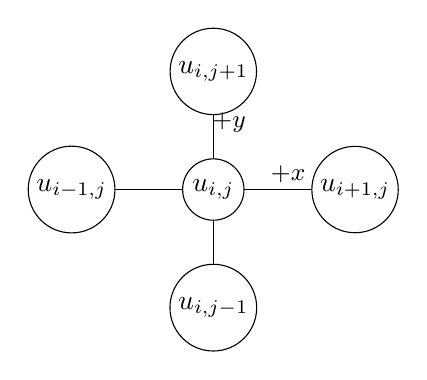
\begin{tikzpicture}[scale=1.0, line cap=round, line join=round]
    % Nodes
    \node[circle, draw, inner sep=2pt] (C) at (0,0) {$u_{i,j}$};
    \node[circle, draw, inner sep=2pt] (N) at (0,1.5) {$u_{i,j+1}$};
    \node[circle, draw, inner sep=2pt] (S) at (0,-1.5) {$u_{i,j-1}$};
    \node[circle, draw, inner sep=2pt] (E) at (1.8,0) {$u_{i+1,j}$};
    \node[circle, draw, inner sep=2pt] (W) at (-1.8,0) {$u_{i-1,j}$};

    % Connections
    \draw[-] (C) -- (N);
    \draw[-] (C) -- (S);
    \draw[-] (C) -- (E);
    \draw[-] (C) -- (W);

    % Direction labels
    \node at (0.95, 0.2) {\small $+x$};
    \node at (0.2, 0.85) {\small $+y$};
  \end{tikzpicture}
  \caption{Five-point finite-difference stencil used for the discrete Laplacian on the two-dimensional Cartesian grid.}
  \label{fig:five_point_stencil}
\end{figure}

The physical interpretation of \eqref{eq:laplacian_5point_numimpl} is straightforward. The value at each interior node is compared with its four nearest neighbors: east, west, north, and south. If the center value is larger than the neighborhood average, diffusion produces a negative contribution; if it is smaller, diffusion produces a positive contribution. In this sense, the discrete Laplacian measures local curvature or local imbalance, and the diffusion term acts to smooth the concentration field over time.

For periodic boundaries, the neighbor indices wrap around at the domain edges. Thus the point left of $i=0$ is identified with $i=N_x-1$, and the point right of $i=N_x-1$ is identified with $i=0$. The same applies in the $y$-direction. In the code, this periodic connectivity is built directly into the diffusion operator itself. This is a central design decision of the project: the Laplacian assembly and stencil application always use periodic connectivity as their internal baseline, while non-periodic boundary conditions are enforced afterward by explicitly overwriting boundary nodes. The boundary treatment will be discussed in detail in a later section; for the present section, the important point is that the spatial operator itself is defined in one consistent periodic form.

The final code realizes the same discrete Laplacian in three mathematically equivalent ways. The first realization is a sparse matrix form, the second is a dense matrix form, and the third is a matrix-free stencil form. Although these implementations differ in storage and application strategy, they all approximate the same operator \eqref{eq:laplacian_5point_numimpl}. This separation between mathematical discretization and software realization is one of the most important ideas of the project.

To derive the matrix form, one first introduces the one-dimensional periodic second-derivative matrix. For a grid with $N$ points, the unscaled operator has the tridiagonal pattern
\begin{equation}
L_{1\mathrm{D}} =
\begin{bmatrix}
-2 & 1  & 0  & \cdots & 0 & 1 \\
1  & -2 & 1  & \ddots &   & 0 \\
0  & 1  & -2 & \ddots & \ddots & \vdots \\
\vdots & \ddots & \ddots & \ddots & 1 & 0 \\
0  &   & \ddots & 1 & -2 & 1 \\
1  & 0 & \cdots & 0 & 1 & -2
\end{bmatrix},
\label{eq:l1d_periodic_numimpl}
\end{equation}
where the corner entries implement the wrap-around coupling required by periodicity. In the code, this operator is assembled by \texttt{buildLaplacian1D\_periodic.m}. It returns the unscaled stencil matrix, and the factors $1/h_x^2$ and $1/h_y^2$ are introduced only when the full two-dimensional operator is built.

Because the state is vectorized in MATLAB column-major order as $u = U(:)$, the two-dimensional Laplacian is assembled by a Kronecker sum:
\begin{equation}
L
=
\frac{1}{h_y^2}\left(I_x \otimes L_y\right)
+
\frac{1}{h_x^2}\left(L_x \otimes I_y\right),
\label{eq:kron_laplacian_numimpl}
\end{equation}
where $L_x$ and $L_y$ are the one-dimensional periodic second-derivative matrices in the $x$- and $y$-directions, and $I_x$, $I_y$ are identity matrices of matching sizes. This formula is implemented in \texttt{buildLaplacian2D.m}. The ordering in \eqref{eq:kron_laplacian_numimpl} is not arbitrary. It is dictated by the mapping
\[
u = U(:),
\]
which stacks matrix columns one after another in MATLAB memory order. The term
\[
\frac{1}{h_y^2}(I_x \otimes L_y)
\]
acts along the rows of each column, while
\[
\frac{1}{h_x^2}(L_x \otimes I_y)
\]
couples corresponding entries across neighboring columns. If the ordering were inconsistent with the vectorization convention, the operator would connect the wrong nodes and the simulation would become physically meaningless. For this reason, the Kronecker structure and the storage layout must always be explained together.

The sparse matrix realization is used when \texttt{p.diffusionMode = "matrix"}. In that case, the operator struct contains the field \texttt{op.L}, and the diffusion contribution is computed by direct sparse matrix--vector multiplication:
\[
\Delta_h u \approx L u.
\]
For the dense realization, selected by \texttt{p.diffusionMode = "full"}, the same operator is stored as a full matrix and applied in the same algebraic way. Numerically, both versions represent the same discrete stencil. The difference lies only in storage format and computational cost. The dense realization is therefore not intended for large practical runs, but it remains useful as a reference implementation on small grids because it exposes the full operator explicitly.

The matrix-free stencil realization is selected by \texttt{p.diffusionMode = "stencil"}, which is the default mode in the final version of the code. In this case, the solver does not store the global matrix $L$. Instead, it stores only the minimal geometric information needed to evaluate the stencil, namely $N_x$, $N_y$, $1/h_x^2$, and $1/h_y^2$. These quantities are built once in \texttt{buildStencil2D.m} and stored in the struct \texttt{op.S}. During each time step, \texttt{applyLaplacianStencil.m} reshapes the vector $u$ into the array $U$, constructs the east, west, north, and south neighbor arrays by circular shifts, evaluates the five-point formula directly, and finally vectorizes the result again:
\[
u \;\rightarrow\; U
\;\rightarrow\; \Delta_h U
\;\rightarrow\; (\Delta_h U)(:).
\]
This approach is mathematically equivalent to matrix multiplication by $L$, but it avoids storing the large global Laplacian explicitly.

The stencil implementation in the final code can therefore be interpreted as a matrix-free realization of exactly the same finite-difference operator. This point is important: the stencil backend is not a different numerical method, and it does not change the discrete model. It is simply a different implementation of the same second-order five-point Laplacian. The project does not compare different spatial discretizations against each other; it compares different realizations of one and the same discretization.

A practical advantage of the stencil form is that its memory requirements are determined mainly by the solution vectors and a very small operator description, rather than by storing the entire sparse or dense matrix. For this reason, the stencil realization is the most suitable default choice for larger problem sizes in the final code. The benchmark chapter later provides the quantitative evidence for this design decision. Here, it is enough to note that the matrix-free stencil keeps the mathematical discretization unchanged while reducing storage overhead in practical runs.

The project also includes internal checks that support the correctness of the discrete Laplacian. Since the five-point stencil is a consistent discretization of the continuous Laplacian, constant fields should produce a zero diffusion contribution. Moreover, the sparse periodic Laplacian has the expected symmetric structure, and the stencil and matrix applications should agree to machine precision when evaluated on the same state. These properties are verified in dedicated test files, including \path{test_laplacian_constant.m}, \path{test_laplacian_symmetry.m}, and \path{test_laplacian_stencil_equivalence.m}. Their role is not to introduce a new numerical method, but to confirm that the implementation matches the intended discrete operator.

In summary, the spatial discretization of diffusion in the final project is based on a standard second-order five-point finite-difference Laplacian on a uniform Cartesian grid. The corresponding discrete operator is realized either as a sparse matrix, a dense matrix, or a matrix-free stencil, but all three forms are algebraically consistent with the same formula. This gives the project both numerical clarity and implementation flexibility: the mathematics remains fixed, while the software can choose the most suitable operator realization for the intended task.

\section{Time Integration and the Full Update Algorithm}
\label{sec:numimpl_time_update}

After spatial discretization, the Gray--Scott system is reduced to a large coupled system of ordinary differential equations in time. Let $u(t)$ and $v(t)$ denote the vectorized concentration fields after spatial discretization. Then the semi-discrete system can be written in the form
\begin{equation}
\frac{d u}{d t} = D_u L u + f_u(u,v),
\qquad
\frac{d v}{d t} = D_v L v + f_v(u,v),
\label{eq:semi_discrete_gs_numimpl}
\end{equation}
where $L$ denotes the discrete Laplacian introduced in the previous section and
\begin{equation}
f_u(u,v) = -u \circ v^2 + F(1-u),
\qquad
f_v(u,v) = u \circ v^2 - (F+k)v.
\label{eq:reaction_vector_form_numimpl}
\end{equation}
Here, $\circ$ denotes componentwise multiplication. The nonlinear reaction term is therefore evaluated pointwise at each grid node, whereas the diffusion term couples neighboring nodes through the discrete Laplacian.

In the final implementation, time integration is performed by the explicit forward Euler method. If $u^n$ and $v^n$ denote the numerical solution at time
\[
t_n = n \,\Delta t,
\]
then one step of the method is
\begin{equation}
u^{n+1}
=
u^n + \Delta t \left(D_u L u^n + f_u(u^n,v^n)\right),
\label{eq:euler_u_numimpl}
\end{equation}
\begin{equation}
v^{n+1}
=
v^n + \Delta t \left(D_v L v^n + f_v(u^n,v^n)\right).
\label{eq:euler_v_numimpl}
\end{equation}
This scheme is first-order accurate in time \cite{leveque2007}. Its main advantage in the present project is its simplicity and transparency. Since the focus of the work is on the implementation and comparison of different diffusion backends, a fully explicit update makes the numerical workflow easy to trace and keeps the effect of each implementation choice clearly visible.

The explicit Euler step is implemented in the file \path{src/core/eulerStep.m}. Its structure follows the mathematical decomposition of the Gray--Scott model very closely. For each time step, the solver computes the diffusion contribution, then the reaction contribution, optionally adds source terms for manufactured-solution verification, advances the state by one explicit step, and finally enforces the selected boundary conditions. In abstract notation, the numerical update used in the code can be written as
\begin{equation}
u^{n+1}
=
\mathcal{B}\!\left(
u^n + \Delta t \left[d_u^n + r_u^n + s_u^n\right]
\right),
\label{eq:update_with_bc_u_numimpl}
\end{equation}
\begin{equation}
v^{n+1}
=
\mathcal{B}\!\left(
v^n + \Delta t \left[d_v^n + r_v^n + s_v^n\right]
\right),
\label{eq:update_with_bc_v_numimpl}
\end{equation}
where $d_u^n$, $d_v^n$ are the diffusion contributions, $r_u^n$, $r_v^n$ are the reaction contributions, $s_u^n$, $s_v^n$ are optional source terms, and $\mathcal{B}$ denotes the boundary overwrite operator applied after the explicit update. When no manufactured source is used, the source vectors are simply zero.

The reaction part is implemented in \path{src/reaction/reactionGrayScott.m}. There the nonlinear product
\[
u \circ v^2
\]
is evaluated componentwise, and the reaction vectors are formed exactly according to \eqref{eq:reaction_vector_form_numimpl}. Since this computation acts locally at each grid node, it does not depend on the chosen diffusion backend. This is an important structural property of the final code: the diffusion realization may change between matrix, dense, and stencil modes, but the reaction update remains identical in all cases.

The diffusion contribution is computed by \path{src/core/applyDiffusion.m}. This function dispatches to the appropriate backend according to the parameter
\[
\texttt{p.diffusionMode} \in \{\texttt{"matrix"},\texttt{"full"},\texttt{"stencil"}\}.
\]
Thus, for each time step, the code evaluates
\[
d_u^n = D_u \Delta_h u^n,
\qquad
d_v^n = D_v \Delta_h v^n,
\]
but the internal realization of $\Delta_h$ depends on the selected operator backend. The time integrator itself does not need to know whether the Laplacian is being applied by sparse matrix multiplication, dense matrix multiplication, or a matrix-free stencil. This is one of the cleanest aspects of the implementation: the one-step update routine is written once, while the diffusion backend is exchanged through a common interface.

In addition to the physical Gray--Scott terms, the final implementation supports optional source terms through the user-defined field \path{p.sourceFcn}. This functionality is used for the manufactured-solution tests included in the verification part of the project. If such a source function is present, the solver evaluates
\[
(s_u^n, s_v^n) = s(x,y,t_n,p)
\]
on the current grid and adds the resulting vectors inside the Euler update. If no source function is defined, the source contribution is set to zero automatically. This design allows the same stepping routine to be used both for ordinary simulation and for verification problems, without modifying the core algorithm.

The temporal update is therefore fully explicit. At each step, all right-hand-side terms are evaluated using the old state $(u^n,v^n)$, and the new state is obtained directly by addition. No nonlinear solve, linear solve, or iterative correction is required. From an implementation perspective, this keeps the code compact and makes the relation between the discrete equations and the program logic very direct.

The price of this simplicity is the usual stability restriction of explicit methods. For the pure diffusion equation discretized by central differences in space and forward Euler in time, a standard sufficient stability condition is
\begin{equation}
\Delta t \le
\frac{1}{2D\left(\dfrac{1}{h_x^2}+\dfrac{1}{h_y^2}\right)},
\label{eq:dt_stability_diffusion_numimpl}
\end{equation}
where $D$ denotes the diffusion coefficient \cite{leveque2007}. In the special case $h_x=h_y=h$, this reduces to
\begin{equation}
\Delta t \le \frac{h^2}{4D}.
\label{eq:dt_stability_diffusion_square_numimpl}
\end{equation}
Since the Gray--Scott model contains two diffusing species, the timestep must satisfy this restriction for both $D_u$ and $D_v$. A practical sufficient choice is therefore
\begin{equation}
\Delta t \le
\min\!\left\{
\frac{1}{2D_u\left(\dfrac{1}{h_x^2}+\dfrac{1}{h_y^2}\right)},
\frac{1}{2D_v\left(\dfrac{1}{h_x^2}+\dfrac{1}{h_y^2}\right)}
\right\}.
\label{eq:dt_stability_gray_scott_numimpl}
\end{equation}
For the full nonlinear Gray--Scott system, this should be interpreted as a diffusion-based practical restriction rather than a complete sharp stability bound, since the reaction terms also influence the timestep limitations. As a result, the admissible timestep becomes more restrictive when the grid is refined, because the discrete diffusion operator scales with $1/h_x^2$ and $1/h_y^2$ \cite{leveque2007}. In practical terms, a smaller mesh spacing improves spatial resolution but reduces the stable explicit timestep. The final project therefore uses conservative timestep choices in the default parameter sets, and timestep-related behavior is checked separately in dedicated verification tests. The detailed quantitative comparison of timestep effects belongs to the verification and benchmark discussion rather than to the present implementation chapter.

Another relevant implementation detail is the distinction between simulation time and step count. The model class stores both quantities explicitly through the fields
\[
\texttt{obj.t}
\qquad \text{and} \qquad
\texttt{obj.n}.
\]
After every successful call to the stepping routine, the time is updated according to
\[
t \leftarrow t + \Delta t,
\]
and the step counter is incremented by one. This provides a clean separation between physical time and iteration number. It also allows plotting and export routines to be triggered at user-defined step intervals such as every $N$ steps, independently of the total final time.

At the level of the \texttt{GrayScottModel} class, one complete step is performed by the method \path{step()}, which calls \path{eulerStep.m}, stores the returned solution vectors, and updates the internal counters. The high-level model object therefore manages the simulation state, while the standalone stepping routine contains the actual numerical formula. This separation keeps the time integrator transparent and avoids duplicating step logic in scripts, tests, and the GUI controller.

The one-step function also returns a diagnostic structure. In the final implementation, this structure contains the minimum and maximum values of both fields after the update, together with a flag indicating whether any \texttt{NaN} or \texttt{Inf} value has occurred. These diagnostics do not modify the method itself, but they make the simulation safer and easier to monitor. Detecting non-finite values immediately is especially useful when parameters or time-step settings are changed during testing.

From an algorithmic viewpoint, the complete update sequence used in one time step can be summarized as follows:
\begin{enumerate}
    \item Start from the current vectors $u^n$ and $v^n$.
    \item Compute the diffusion contributions with the selected backend.
    \item Compute the nonlinear reaction contributions pointwise.
    \item Add optional source terms if a manufactured-solution test is active.
    \item Form the explicit Euler update for both fields.
    \item Overwrite boundary nodes according to the selected boundary-condition specification.
    \item Compute diagnostics and advance the stored simulation time and step counter.
\end{enumerate}
This sequence reflects the actual structure of the final code and provides a direct bridge between the semi-discrete equations and the software implementation.

In summary, the time integration in the final project is based on a first-order explicit Euler method applied to the semi-discrete Gray--Scott system. The method is simple, fully transparent, and implemented in a modular way: diffusion, reaction, optional source terms, boundary enforcement, and diagnostics are handled in separate components but combined in one consistent update routine. This design keeps the numerical method clear while allowing the implementation to support verification features and multiple diffusion backends without changing the time-stepping logic.

\section{Boundary-Condition Treatment}
\label{sec:numimpl_boundary_conditions}

In the final implementation, boundary conditions are handled in a way that keeps the diffusion backend, the time integrator, and the user interface consistent with each other. The code supports boundary conditions independently on the four sides of the rectangular domain,
\[
\texttt{left},\quad \texttt{right},\quad \texttt{bottom},\quad \texttt{top},
\]
through the parameter structure \path{p.BC}. For each side, the user may select one of the three types
\[
\texttt{periodic},\qquad \texttt{dirichlet},\qquad \texttt{neumann}.
\]
Periodic boundaries are the default configuration, but Dirichlet and Neumann conditions can be chosen separately on each side. This design makes the solver flexible without changing the underlying grid or the main time-stepping routine.

The boundary-condition handling is normalized in \path{src/core/finalizeParams.m}. If a boundary specification is missing, it is completed automatically with safe defaults. In particular, all four sides are initialized as periodic, the default Dirichlet mode is \path{initial}, and the default Neumann mode is \path{constant}. This normalization step ensures that the subsequent numerical routines always receive a complete and validated boundary-condition structure.

The essential implementation idea is that the discrete diffusion operator itself is built with periodic connectivity, while non-periodic boundary conditions are enforced afterward by explicit overwrite of the boundary nodes. Thus, the diffusion operator remains the same mathematical object across all solver backends, and boundary handling is treated as a separate layer in the update process. This choice is especially useful in a code base that supports sparse-matrix, dense-matrix, and matrix-free stencil realizations of the same Laplacian, because it avoids having to build a different operator for every possible combination of side conditions.

After one explicit Euler step has been formed, the function \path{src/core/applyBoundaryConditions.m} reshapes the state vectors into two-dimensional arrays,
\[
U = \mathrm{reshape}(u,N_y,N_x),
\qquad
V = \mathrm{reshape}(v,N_y,N_x),
\]
and then overwrites the relevant boundary entries according to the selected side conditions. The side conventions used throughout the code are
\[
\texttt{left}: U(:,1), \qquad
\texttt{right}: U(:,N_x),
\]
\[
\texttt{bottom}: U(1,:), \qquad
\texttt{top}: U(N_y,:),
\]
with the same layout used for the field $V$. This explicit convention is important because all boundary operations, tests, and GUI selections rely on the same indexing scheme.

If a side is periodic, no overwrite is performed. The periodic coupling is already built into the discrete Laplacian through the wrap-around structure of the operator. In other words, for periodic boundaries the diffusion step itself already uses the correct neighboring values across the domain edges, so no additional enforcement is necessary after the time update.

For Dirichlet boundaries, the boundary values are imposed strongly by direct assignment after each explicit time step. If the prescribed boundary value is denoted by $g$, then the code sets
\begin{equation}
U(:,1) = g_{\mathrm{left}},
\qquad
U(:,N_x) = g_{\mathrm{right}},
\label{eq:dirichlet_lr_numimpl}
\end{equation}
for left and right boundaries, and
\begin{equation}
U(1,:) = g_{\mathrm{bottom}},
\qquad
U(N_y,:) = g_{\mathrm{top}}.
\label{eq:dirichlet_bt_numimpl}
\end{equation}
The same overwrite is applied separately to the $V$ field, so the concentrations of the two species may be prescribed independently. This is the standard finite-difference treatment of Dirichlet conditions, in which the boundary node values are set directly to the prescribed data \cite{leveque2007}. In the final code, Dirichlet boundaries support two modes. In \path{constant} mode, the user provides fixed values through
\[
\texttt{p.BC.<side>.dirichletValue.u},
\qquad
\texttt{p.BC.<side>.dirichletValue.v}.
\]
In \path{initial} mode, the corresponding boundary values are frozen from the initial condition and then reused at every subsequent step. This is implemented through a boundary cache, \path{p.BCcache}, which is created when the model is initialized or reset. As a result, the code can preserve initial edge values exactly without recomputing them later.

For Neumann boundaries, the implementation uses first-order one-sided finite differences \cite{leveque2007}. If the outward normal derivative is prescribed as
\[
\frac{\partial u}{\partial n} = g,
\]
then the boundary value is reconstructed from the adjacent interior value. On the left boundary, the discrete condition is
\begin{equation}
\frac{U(:,2)-U(:,1)}{h_x} = g_{\mathrm{left}},
\label{eq:neumann_left_numimpl}
\end{equation}
which gives
\begin{equation}
U(:,1) = U(:,2) - h_x g_{\mathrm{left}}.
\label{eq:neumann_left_update_numimpl}
\end{equation}
Similarly, on the right boundary,
\begin{equation}
\frac{U(:,N_x)-U(:,N_x-1)}{h_x} = g_{\mathrm{right}},
\label{eq:neumann_right_numimpl}
\end{equation}
so that
\begin{equation}
U(:,N_x) = U(:,N_x-1) + h_x g_{\mathrm{right}}.
\label{eq:neumann_right_update_numimpl}
\end{equation}
For the bottom and top boundaries, the corresponding formulas are
\begin{equation}
U(1,:) = U(2,:) - h_y g_{\mathrm{bottom}},
\qquad
U(N_y,:) = U(N_y-1,:) + h_y g_{\mathrm{top}}.
\label{eq:neumann_vertical_update_numimpl}
\end{equation}
Again, the same construction is applied independently to the $V$ field. In the present implementation, Neumann boundaries are supported in \path{constant} mode, meaning that the user prescribes constant normal derivatives on each side.

This boundary treatment is integrated into the one-step update described in the previous section. If $\widetilde{u}^{\,n+1}$ and $\widetilde{v}^{\,n+1}$ denote the provisional Euler update before boundary enforcement, then the final stored state is
\begin{equation}
u^{n+1} = \mathcal{B}\!\left(\widetilde{u}^{\,n+1}\right),
\qquad
v^{n+1} = \mathcal{B}\!\left(\widetilde{v}^{\,n+1}\right),
\label{eq:bc_overwrite_operator_numimpl}
\end{equation}
where $\mathcal{B}$ denotes the overwrite operation defined by the selected side conditions. In this way, boundary enforcement is performed strongly after every time step. The update does not rely on weak penalization or embedded ghost-cell iterations; instead, the prescribed boundary behavior is imposed directly on the stored state arrays.

A practical consequence of this design is that all diffusion backends remain compatible with the same boundary-condition routine. The sparse matrix mode, the dense matrix mode, and the stencil mode all produce a provisional diffusion update using the same periodic baseline operator. Boundary conditions are then enforced in exactly the same way, independently of how the Laplacian was applied. This is one of the main reasons why matrix and stencil solutions can be compared cleanly: the backend changes only the realization of diffusion, not the surrounding enforcement logic.

The implementation also supports mixed boundary configurations. For example, one side may be Dirichlet, another Neumann, and the remaining sides periodic. This capability is verified in \path{tests/test_boundary_conditions.m}, where constant Dirichlet enforcement, Neumann derivative enforcement, and mixed boundary configurations are checked across all three diffusion modes. These tests confirm that the same boundary rules are applied consistently in the matrix, stencil, and dense implementations.

From a numerical perspective, the chosen approach is primarily an implementation strategy rather than a change of the underlying model. Periodic boundaries are incorporated directly into the operator, while Dirichlet and Neumann conditions are imposed by explicit update of the edge nodes after each step. This gives the project a simple and robust boundary framework: the operator construction remains uniform, the user can switch boundary types per side, and the final stored state always satisfies the selected edge conditions exactly at the discrete level.

In summary, the final code uses a hybrid boundary-handling design. Periodic boundaries are encoded directly in the discrete Laplacian, whereas Dirichlet and Neumann conditions are enforced strongly by post-step overwrite on the two-dimensional state arrays. The result is a boundary-condition implementation that is flexible, backend-independent, and consistent with the modular structure of the solver.

\section{Diffusion Backends and Default Solver Choice}
\label{sec:numimpl_backends_selection}

The project supports three realizations of the discrete diffusion operator, selected through the parameter
\[
\texttt{p.diffusionMode} \in \{\texttt{"matrix"},\texttt{"full"},\texttt{"stencil"}\}.
\]
All three options represent the same second-order finite-difference Laplacian introduced in Section~\ref{sec:numimpl_spatial_laplacian}. They do not change the mathematical model, the computational grid, or the time integrator. Instead, they differ only in how the discrete operator is stored and applied in the code. This distinction is central to the project, because the main implementation question is not which diffusion model to use, but which realization of the same model is most suitable in practice.

The construction of the operator is handled by \path{src/core/makeOperator.m}. This function inspects the selected diffusion mode and prepares a backend-specific operator structure before the time loop begins. As a result, the cost of building the operator is paid only once during initialization, rather than being repeated at every time step. This is an important implementation choice, since the diffusion operator depends only on the grid and the selected backend, not on the evolving concentrations themselves. Preconstructing the operator therefore avoids unnecessary repeated work during simulation.

If the mode is set to \path{matrix}, the function \path{src/operators/buildLaplacian2D.m} assembles the two-dimensional periodic Laplacian as a sparse matrix. This matrix is stored in the field \path{op.L}, and the diffusion contribution is evaluated by sparse matrix--vector multiplication. The sparse backend is algebraically explicit and closely reflects the Kronecker-sum formulation of the operator. It is therefore convenient for verification, inspection, and direct comparison with the other backends. At the same time, it requires storage not only for the numerical values of the operator, but also for the sparse index structure used by MATLAB to represent the matrix efficiently.

If the mode is set to \path{full}, the same operator is converted to a dense matrix representation and stored explicitly. The diffusion term is then evaluated by ordinary dense matrix--vector multiplication. This mode is not intended for large-scale simulation, because a dense matrix for a two-dimensional Laplacian quickly becomes prohibitively expensive in memory. Its main role in the final code is therefore as a small-grid reference realization. Since the operator is stored completely and explicitly, it can be useful for debugging, sanity checks, and direct comparison on small problem sizes. For serious production runs, however, the dense backend is not the preferred choice.

If the mode is set to \path{stencil}, no global Laplacian matrix is stored. Instead, the code constructs a compact description of the operator in \path{src/operators/buildStencil2D.m}, containing only the information needed to evaluate the five-point stencil directly on the grid. During each step, \path{src/core/applyDiffusion.m} calls \path{src/operators/applyLaplacianStencil.m}, which reshapes the vectorized state into a two-dimensional array, forms the neighboring values by periodic shifts, evaluates the stencil locally, and vectorizes the result again. This backend is therefore matrix-free: it applies the same discrete operator without ever assembling the full global matrix.

The three backends can be summarized conceptually as follows:
\begin{itemize}
    \item \path{matrix}: sparse global operator, applied by sparse matrix--vector multiplication;
    \item \path{full}: dense global operator, applied by dense matrix--vector multiplication;
    \item \path{stencil}: matrix-free local operator evaluation on the grid.
\end{itemize}
Although these realizations are different computationally, they remain mathematically equivalent at the discrete level. The same five-point Laplacian is used in all cases, and the same explicit Euler update is applied afterward. This makes it possible to compare the backends fairly, since any observed difference comes from the implementation strategy rather than from a change in the numerical scheme.

A major advantage of the final architecture is that all three backends are accessed through the same interface. The time-stepping routine \path{src/core/eulerStep.m} does not contain separate logic for sparse, dense, and stencil diffusion. Instead, it calls the common helper \path{src/core/applyDiffusion.m}, which dispatches internally to the appropriate backend. This design keeps the step routine compact and avoids code duplication. It also improves maintainability: backend-specific changes remain localized in the operator layer and do not propagate through the rest of the solver.

The project includes dedicated consistency tests to verify that these backends produce the same discrete diffusion action up to machine precision when applied to the same state. In particular, the stencil and matrix realizations are checked against each other, and the resulting equivalence confirms that the stencil mode is not an approximation of lower quality, but simply a different realization of the same operator. This is a key point for the implementation logic of the project. The choice of backend affects memory use and computational cost, but not the underlying finite-difference discretization.

In the final version of the project, the stencil backend is selected as the default diffusion mode. This choice was made for practical computational reasons. The sparse-matrix realization already reduces storage compared with a dense matrix, but it still requires an explicitly assembled global operator together with its sparse indexing structure. The stencil realization avoids this global matrix storage entirely and therefore has lower structural overhead. Its memory footprint is determined mainly by the state vectors and a small set of geometric coefficients, rather than by the storage of the full operator itself.

This property becomes more important as the grid size increases. For a two-dimensional problem with
\[
N = N_x N_y
\]
degrees of freedom per species, a dense matrix representation scales like \(O(N^2)\) in storage and is therefore unsuitable except for very small test cases. The sparse representation reduces this to \(O(N)\) nonzero storage, but still carries the overhead associated with explicit matrix representation. The stencil realization also scales effectively with \(O(N)\) in the size of the evolving fields, but without storing the global Laplacian matrix. For this reason, it is the most natural choice when the objective is to keep the solver practical for larger grids while preserving the same discrete method.

The benchmark study presented later in the report provides the quantitative evidence for this decision. In that study, the stencil backend shows a more favorable practical memory behavior for larger problem sizes, and its measured memory use remains closer to the expected low-storage behavior of a matrix-free implementation. For the present chapter, it is sufficient to state the implementation consequence: the final code uses the stencil backend as the default solver because it preserves the same numerical discretization while reducing storage overhead in practical runs.

The existence of multiple backends is not only useful for performance considerations, but also for software reliability. The sparse matrix mode provides a clear algebraic reference implementation, the dense mode provides a fully explicit small-scale reference, and the stencil mode provides the preferred production backend. This layered design makes the code easier to verify. When two independently implemented realizations of the same operator agree numerically, confidence in the correctness of the solver increases significantly.

Another important implementation aspect is that the default backend choice is propagated consistently through the whole project. The default parameter set selects \path{stencil}, the main non-GUI runner uses the same default, and the graphical user interface is aligned with that choice as well. As a result, the user sees one coherent solver behavior across scripts, tests, and interactive runs. The backend is still switchable when comparison or debugging is needed, but the default configuration reflects the preferred practical implementation.

From a software-engineering perspective, this backend design captures one of the main contributions of the project. The solver is not restricted to a single hard-coded operator realization. Instead, it provides a common simulation framework in which multiple mathematically equivalent diffusion backends can be tested, validated, and compared under identical conditions. This makes the implementation both more flexible and more informative than a single-backend code base.

In summary, the final project implements three realizations of the same discrete Laplacian: a sparse matrix backend, a dense matrix backend, and a matrix-free stencil backend. Among these, the stencil backend is chosen as the default because it avoids storing the global diffusion matrix, reduces structural memory overhead, and remains fully consistent with the same finite-difference scheme used by the other realizations. The result is a solver framework that combines numerical consistency with practical flexibility and backend-aware implementation design.

\section{MATLAB Implementation Architecture and Practical Optimizations}
\label{sec:numimpl_architecture_optimizations}

Beyond the numerical method itself, an important part of the project is the way the solver is organized as a MATLAB program. The final implementation is written in MATLAB R2025b and is structured as a modular code base rather than as a single monolithic script. This design choice improves readability, simplifies testing, and makes it possible to modify one component of the program without changing the rest of the solver. In particular, parameter definition, grid generation, diffusion-operator construction, reaction evaluation, one-step time integration, plotting, output export, and testing are separated into dedicated files with clearly defined responsibilities.

The code base is organized into several functional layers. The directory \path{src/core} contains the central numerical workflow, including parameter normalization, grid construction, diffusion dispatch, time stepping, initial conditions, and boundary enforcement. The directory \path{src/operators} contains the different realizations of the discrete Laplacian. The directory \path{src/reaction} contains the Gray--Scott reaction term, while \path{src/model} contains the class \path{GrayScottModel.m}, which encapsulates the complete simulation state. Input/output functionality, such as plotting and frame export, is placed in \path{src/io}. The GUI is stored separately in \path{scripts/GrayScottController.mlapp}, and the verification and benchmark routines are kept in the \path{tests} directory. This separation of concerns keeps the numerical core independent from the interface and from the testing framework.

At the entry-point level, the project provides two main launchers. The script \path{run_model_class.m} executes the simulation in a non-GUI mode and is suited for reproducible scripted runs, saved output, and batch-like testing. The script \path{run_gui.m} launches the graphical interface. Both entry points add the required source folders to the MATLAB path and then rely on the same underlying core functions. This is an important architectural decision: the GUI is not a separate solver, but only a controller layer that accesses the same numerical engine as the non-GUI execution path. As a result, scripted runs, tests, and interactive runs remain consistent with each other.

The parameter workflow is deliberately staged. The function \path{defaultParams.m} defines a complete parameter set with physically meaningful defaults, including grid size, diffusion coefficients, feed and kill parameters, timestep, final time, plotting cadence, file output cadence, initial-condition type, random seed, boundary-condition defaults, and the selected diffusion backend. After that, \path{finalizeParams.m} validates and normalizes the user-edited parameter structure. This second step is important because users or scripts may modify only part of the parameter set. The normalization step therefore guarantees that missing or incomplete settings are completed with valid defaults before the simulation begins. In particular, the diffusion mode is checked, and the boundary-condition structure is expanded into a complete four-sided representation.

The next architectural step is grid construction. The function \path{buildGrid.m} computes the mesh spacing, the coordinate vectors, and the two-dimensional mesh arrays associated with the problem domain. The grid object is then passed explicitly into the model constructor. This means that the model does not hide the domain geometry internally or rebuild it implicitly. Instead, the grid is treated as a first-class object in the simulation pipeline. This improves transparency and ensures that the diffusion operator and the state initialization are built on the same geometric information.

The central state container is the class \path{src/model/GrayScottModel.m}. This class stores the parameter structure, the grid, the selected diffusion operator, the current solution vectors, the current simulation time, and the current step index. The class-based design provides a clean separation between persistent simulation state and the numerical update logic. The state variables \path{u} and \path{v} are kept inside the object, while the actual update formula is implemented in the external function \path{eulerStep.m}. This avoids repeating state-management code in different scripts and makes the model behavior uniform across GUI runs, non-GUI runs, and tests.

The constructor of \path{GrayScottModel} performs three important tasks. First, it validates and stores the parameter structure. Second, it constructs the diffusion operator once through the backend-specific operator builder. Third, it initializes the concentration fields and stores them as vectorized state variables. This means that the costly operator setup is separated from the repeated time-stepping phase. Once the model object has been created, the simulation loop only applies the already constructed operator and advances the state. This is one of the main implementation optimizations of the project: objects that depend only on the grid and the chosen backend are created once and then reused throughout the simulation.

The model initialization also contains an explicit reproducibility measure. If the parameter structure includes a seed, the constructor uses
\[
\texttt{rng(p.seed,"twister")}
\]
before generating the initial condition. As a result, the random perturbations used in the baseline and Pearson-style initial conditions are reproducible across runs. This is essential for meaningful backend comparison, GUI/non-GUI consistency testing, and benchmark reproducibility. Without a controlled seed, two runs with identical nominal parameters could produce slightly different pattern development simply because the initial perturbation differed.

Another implementation detail with practical importance is the boundary cache used for Dirichlet conditions in \path{initial} mode. When the model is initialized, the code stores the initial values along the left, right, bottom, and top boundaries in the structure \path{p.BCcache}. These cached values are then reused whenever the corresponding boundary must remain equal to the initial state. This avoids recomputing or reconstructing those values later and guarantees that the Dirichlet condition remains exactly consistent with the initially generated fields. The cache therefore serves both correctness and clarity.

The one-step evolution itself is intentionally modular. The function \path{eulerStep.m} receives the current state vectors, the operator structure, the parameter struct, and the current time. It then computes diffusion, reaction, optional manufactured source terms, the explicit Euler update, and boundary enforcement. Since the diffusion contribution is obtained through the helper \path{applyDiffusion.m}, the time-stepper remains independent of the selected backend. This modularity has a direct software benefit: modifications to the operator implementation do not require changes to the reaction code or to the time integrator, as long as the common diffusion interface is preserved.

A related architectural strength of the project is its separation between numerical logic and visualization logic. The functions \path{plotState.m} and \path{exportFrame.m} are placed in \path{src/io} and do not modify the numerical solution. They operate only on already computed states. This separation is useful because it prevents plotting code from becoming entangled with the solver itself. The numerical result is therefore independent of whether live plotting or PNG export is enabled.

The implementation also contains several practical optimizations that improve runtime behavior or software robustness without changing the numerical method.

A first optimization is the reuse of graphics objects during live plotting. In \path{plotState.m}, persistent handles are used for the image and the colorbar. Instead of recreating the plot from scratch at every update, the code updates only the displayed image data through the \path{CData} property. This reduces repeated graphics-object creation and makes live visualization more efficient, especially for long runs with many output frames.

A closely related optimization is used in \path{exportFrame.m}. There, the code maintains a persistent invisible figure, axis, and image object. When a new snapshot is exported, the figure is not recreated; only the image content and title are updated before printing the result to PNG. This is more efficient and more robust than repeatedly opening and closing figures during a long simulation. The code also uses
\[
\texttt{print(...,"-dpng","-r300")}
\]
instead of simpler export commands, which improves the reliability and quality of generated PNG files.

Another optimization is the separation between plotting cadence and simulation cadence. The parameter \path{plotEvery} determines how often live visualization is updated, while \path{savePngEvery} controls how often PNG frames are exported. The numerical time step itself is unaffected by these values. This prevents expensive visualization from being performed at every step unless explicitly requested. In practice, the simulation may advance through many internal Euler steps while plotting only every twentieth step and exporting only every fiftieth step. Such decoupling is important because visualization frequency should be a user-controlled output setting rather than an implicit part of the solver algorithm.

The non-GUI runner \path{run_model_class.m} also includes reproducibility-oriented output management. For each run, it creates a timestamped output directory, stores a metadata file containing the parameters, MATLAB version, and platform information, writes a human-readable log file, and saves the final state to a MAT file. These measures do not alter the numerical solution, but they make the results traceable and easier to reproduce later. In a project where solver variants are benchmarked and compared, this output discipline is an important implementation choice.

The code contains additional robustness features intended to catch problems early. Input validation is used in several helper functions to verify that required fields are present and that dimensions are consistent. The step routine returns diagnostic information such as extrema and a flag for \path{NaN} or \path{Inf} values. The non-GUI runner checks this flag inside the main loop and stops immediately if non-finite values are detected. Such safeguards do not improve the mathematical order of the method, but they do improve the reliability of the software during testing and parameter exploration.

The project architecture also benefits from having multiple independent ways to exercise the same numerical core. The tests in the \path{tests} directory check Laplacian properties, stencil--matrix equivalence, timestep behavior, spatial convergence, mixed boundary conditions, manufactured-solution cases, Pearson-style pattern sanity, and GUI/non-GUI consistency. Because the solver components are modular, these tests can target specific layers of the program rather than only the complete application as a black box. This is one of the strengths of the implementation: correctness is supported not only by the final visual patterns, but also by structured verification of individual numerical and software components.

Although the GUI is not the focus of this chapter, it is worth noting its architectural role briefly. The App Designer file \path{GrayScottController.mlapp} is primarily a control and visualization layer. It allows the user to edit parameters, select presets, start or stop runs, reset the model, switch boundary types, and choose the diffusion backend. However, it does not replace the underlying numerical engine. Instead, it passes user choices into the same parameter and model infrastructure used by the non-GUI path. This keeps the implementation coherent: the interactive front end and the scripted solver remain two ways of using one common simulation core.

From a software-engineering perspective, the final implementation combines modularity, reproducibility, and optimization. The code avoids unnecessary rebuilding of operators, reuses graphics objects where repeated output is needed, isolates visualization from the solver, stores metadata for later comparison, and keeps backend-specific logic confined to a limited part of the code base. None of these decisions changes the mathematical scheme, but together they make the final solver more usable, easier to verify, and more suitable for systematic comparison.

In summary, the MATLAB implementation is organized around a clear division of responsibilities: parameter definition and normalization, grid construction, operator setup, model-state management, one-step evolution, output handling, and testing are all separated into dedicated components. On top of this modular architecture, the final code introduces several practical optimizations, including preconstructed operators, reproducible initialization, boundary caching, persistent plotting objects, persistent export figures, and structured output logging. These implementation choices complement the numerical method and help turn the solver into a consistent and reliable computational tool.



\chapter{Code Used in Original/Adopted Form}
\label{sec:code_used_external_software}

\begin{itemize}
    \item \textbf{MATLAB:} MATLAB was the main software environment used to implement, execute, test, and benchmark the Gray--Scott simulation code. All numerical routines, verification scripts, benchmark programs, and export utilities of this project were developed and run in MATLAB.

    \item \textbf{MATLAB App Designer:} App Designer was used to build the graphical user interface of the project. It provides interactive control of model parameters, simulation start and restart actions, plotting options, and access to export functions.

    \item \textbf{VideoWriter:} MATLAB's built-in \texttt{VideoWriter} interface was used to export time-dependent simulation results as video files. This was used for recording the temporal evolution of patterns generated by the Gray--Scott model.

    \item \textbf{\LaTeX:} \LaTeX{} was used to write, structure, and format the final PPP report. It was used for the complete document preparation, including equations, figures, tables, and references.

    \item \textbf{TUBAF \LaTeX{} template:} The official TUBAF report template was used as the formatting basis of the written report. It provided the required layout and document structure for the submission.

    \item \textbf{Bib\TeX{} bibliography workflow:} A bibliography toolchain was used to manage and format the references cited in the report. This made it possible to organize the literature sources consistently and include them automatically in the final document.
\end{itemize}
\chapter{Usage of Chatbots}
\label{chap:tools_ai_usage}

The integration of chatbots powered by advanced language models has become increasingly useful in project-based work. Such tools can provide rapid, context-aware assistance in technical and writing-related tasks, help identify possible issues, and support the preparation of structured documentation. Their ability to respond to natural-language queries and generate relevant suggestions can improve efficiency during development and reporting, provided that their output is reviewed critically and not used without verification.

In the context of this project, chatbot-based and AI-assisted tools were used in a limited and supportive role. In particular, ChatGPT and Gemini were used for several tasks during the development of the code and the preparation of the report. Grammarly was also used as an auxiliary language-support tool during the writing process.

The main areas of use were the following:
\begin{itemize}
    \item \textbf{Code review:} Chatbot support was used to review parts of the MATLAB code, identify possible weaknesses, and suggest improvements in structure, clarity, or consistency.

    \item \textbf{Debugging support:} The tools were used to discuss possible causes of errors, unexpected behavior, or implementation problems and to generate suggestions for resolving them.

    \item \textbf{Code comments:} Assistance was used in formulating or improving code comments so that the implementation became easier to read and understand.

    \item \textbf{Report writing in \LaTeX:} Chatbot support was used to help formulate technical text and convert report content into well-structured \LaTeX{} code during the preparation of the written report.

    \item \textbf{Language support:} Grammarly was used in a limited way to support wording, grammar, and language refinement in the final report.
\end{itemize}

The use of these tools was restricted to supportive assistance only. No chatbot-generated code was adopted directly without modification. Instead, suggestions were reviewed, adapted, and rewritten before being incorporated into the project. Likewise, no generated report text was inserted unchanged into the final document; all written content was manually revised and edited before inclusion in the final submission. All parts of the project, including the implementation, results, code comments, and report text, were manually checked before inclusion in the final submission.

Overall, the use of chatbots and AI-assisted language tools improved the efficiency of selected parts of the workflow, especially in code review, debugging discussion, commenting, and report preparation. However, the final technical decisions, implementation, verification, interpretation of results, and wording of the report remained entirely under manual responsibility.
\chapter{Program Flowchart}
\label{sec:numimpl_flowchart}

The execution structure of the final program is summarized in Figures~\ref{fig:program_flow_setup} and \ref{fig:program_flow_loop}. The first flowchart shows the initialization phase, and the second shows the repeated simulation loop.

\begin{figure}[htbp]
\centering
\footnotesize
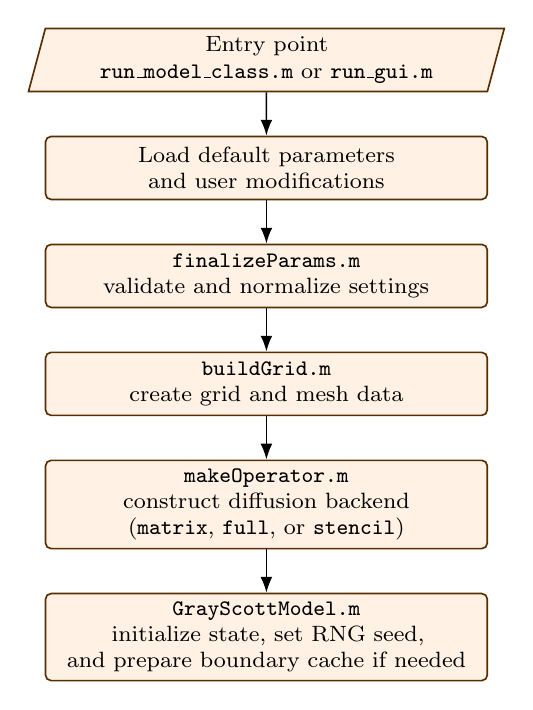
\begin{tikzpicture}[
    node distance=5.5mm,
    >=Latex,
    line width=0.6pt,
    every node/.style={font=\footnotesize},
    box/.style={
        rectangle,
        rounded corners=2pt,
        draw=orange!35!black,
        fill=orange!10,
        align=center,
        text width=5.4cm,
        minimum height=8mm,
        inner sep=3pt
    },
    io/.style={
        trapezium,
        trapezium left angle=75,
        trapezium right angle=105,
        draw=orange!35!black,
        fill=orange!10,
        align=center,
        text width=5.4cm,
        minimum height=8mm,
        inner sep=3pt
    },
    flow/.style={->, draw=black}
]

\node[io] (entry) {Entry point\\ \texttt{run\_model\_class.m} or \texttt{run\_gui.m}};
\node[box, below=of entry] (params) {Load default parameters\\ and user modifications};
\node[box, below=of params] (finalize) {\texttt{finalizeParams.m}\\ validate and normalize settings};
\node[box, below=of finalize] (grid) {\texttt{buildGrid.m}\\ create grid and mesh data};
\node[box, below=of grid] (op) {\texttt{makeOperator.m}\\ construct diffusion backend\\ (\texttt{matrix}, \texttt{full}, or \texttt{stencil})};
\node[box, below=of op] (model) {\texttt{GrayScottModel.m}\\ initialize state, set RNG seed,\\ and prepare boundary cache if needed};

\draw[flow] (entry) -- (params);
\draw[flow] (params) -- (finalize);
\draw[flow] (finalize) -- (grid);
\draw[flow] (grid) -- (op);
\draw[flow] (op) -- (model);

\end{tikzpicture}
\caption{Initialization and setup phase of the final Gray--Scott solver.}
\label{fig:program_flow_setup}
\end{figure}

\begin{figure}[htbp]
\centering
\footnotesize
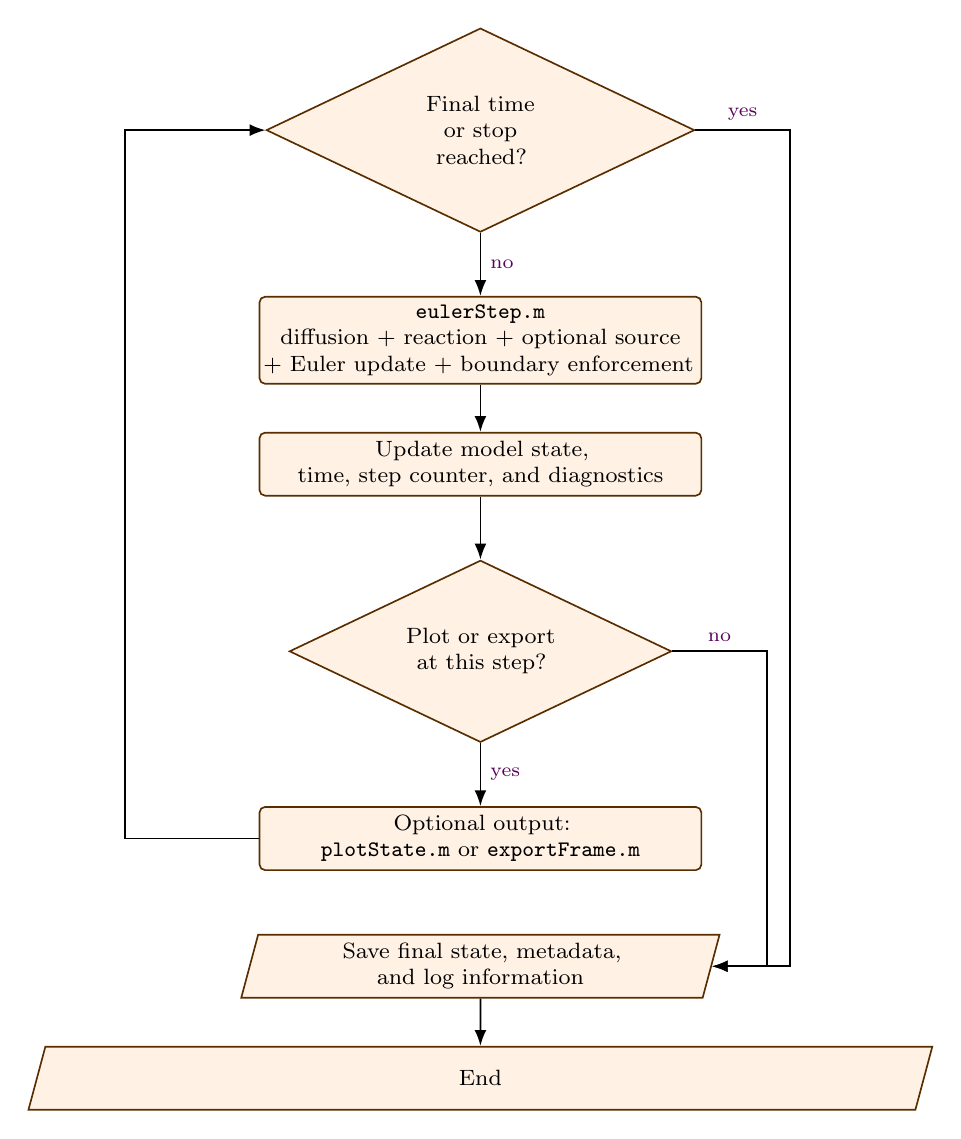
\begin{tikzpicture}[
    node distance=6mm,
    >=Latex,
    line width=0.6pt,
    every node/.style={font=\footnotesize},
    box/.style={
        rectangle,
        rounded corners=2pt,
        draw=orange!35!black,
        fill=orange!10,
        align=center,
        text width=5.4cm,
        minimum height=8mm,
        inner sep=3pt
    },
    decision/.style={
        diamond,
        draw=orange!35!black,
        fill=orange!10,
        align=center,
        aspect=2.1,
        text width=3.3cm,
        inner sep=1.5pt
    },
    io/.style={
        trapezium,
        trapezium left angle=75,
        trapezium right angle=105,
        draw=orange!35!black,
        fill=orange!10,
        align=center,
        text width=5.4cm,
        minimum height=8mm,
        inner sep=3pt
    },
    flow/.style={->, draw=black},
    yn/.style={font=\scriptsize, text=violet!70!black}
]

\node[decision] (stopq) {Final time\\ or stop\\ reached?};
\node[box, below=8mm of stopq] (step) {\texttt{eulerStep.m}\\ diffusion + reaction + optional source\\ + Euler update + boundary enforcement};
\node[box, below=of step] (update) {Update model state,\\ time, step counter, and diagnostics};
\node[decision, below=8mm of update] (outputq) {Plot or export\\ at this step?};
\node[box, below=8mm of outputq] (output) {Optional output:\\ \texttt{plotState.m} or \texttt{exportFrame.m}};
\node[io, below=8mm of output] (save) {Save final state, metadata,\\ and log information};
\node[io, below=of save] (end) {End};

\draw[flow] (stopq) -- node[right, yn] {no} (step);
\draw[flow] (step) -- (update);
\draw[flow] (update) -- (outputq);
\draw[flow] (outputq) -- node[right, yn] {yes} (output);

\draw[flow] (output.west) -- ++(-1.7,0) |- ([xshift=-7mm]stopq.west) -- (stopq.west);
\draw[flow] (outputq.east) -- ++(1.2,0) node[midway, above, yn] {no} |- (save.east);
\draw[flow] (stopq.east) -- ++(1.2,0) node[midway, above, yn] {yes} |- (save.east);
\draw[flow] (save) -- (end);

\end{tikzpicture}
\caption{Repeated simulation loop of the final Gray--Scott solver.}
\label{fig:program_flow_loop}
\end{figure}
\chapter{Testing for Verification}
\label{chap:verification}

\section{Verification strategy}
\label{sec:verification_strategy}

This chapter documents the test cases used to verify the correctness and consistency of the implemented Gray--Scott solver. The focus is on \emph{verification}, i.e.\ checking whether the numerical methods and their implementation solve the intended discrete problem correctly. In accordance with the PPP guideline, the chapter therefore emphasizes reproducible test cases with clearly defined aims, setups, execution procedures, expected results, and obtained results.

The verification strategy is organized in several layers. First, low-level operator tests are used to verify the correctness and convergence of the discrete diffusion operator. Second, time-integration tests check whether the explicit Euler method shows the expected temporal behavior. Third, boundary-condition tests confirm that Dirichlet and Neumann boundary conditions are imposed correctly in the implemented formulations. Fourth, equivalence tests compare different implementation variants, especially the matrix-based and stencil-based diffusion operators, in order to verify that they produce consistent results. Finally, interface-level consistency tests are used to check that the GUI execution path reproduces the same numerical results as the non-GUI reference workflow.

Besides these formal verification tests, the project also includes a validation-oriented pattern sanity check based on a Pearson-type Gray--Scott setup. This test is not a strict proof of numerical correctness in the sense of manufactured-solution verification, but it provides an additional qualitative sanity check that the implemented model reproduces physically plausible pattern-forming behavior. Since validation is not mandatory in the PPP guideline, such tests are treated here as supportive evidence rather than as the main verification basis.

Overall, the chapter is designed to move from rigorous numerical verification of core building blocks toward consistency checks of the full implementation. This layered structure is important because correctness of the final simulation results depends not only on the governing equations, but also on the correct interaction of operator assembly, time stepping, boundary treatment, solver implementation, and user interface execution.

\section{Detailed Verification Test Cases}
\label{sec:verification_detailed_cases}

\subsection{Test Case 1: MMS operator convergence of the discrete Laplacian}
\label{sec:verification_testcase_mms_operator}

\paragraph{Aim.}
This test case verifies the spatial accuracy of the discrete Laplacian operator implemented in the code. The purpose is to check that the matrix-based finite-difference Laplacian produced by \texttt{buildLaplacian2D} converges with the expected second-order accuracy on a sequence of refined grids when it is applied to a smooth exact solution. Since the Laplacian operator is one of the core building blocks of the Gray--Scott solver, this is a fundamental verification step.

\paragraph{Setup.}
The test uses the Method of Manufactured Solutions (MMS). A smooth periodic exact solution is prescribed on the square domain
\[
\Omega = [0,1)\times[0,1)
\]
with periodic boundary conditions in both spatial directions. The manufactured fields are
\[
u^\ast(x,y,t) = 1.0 + 0.1\cos\!\bigl(2\pi(2x+3y)+t\bigr),
\]
\[
v^\ast(x,y,t) = 0.5 + 0.1\cos\!\bigl(2\pi(2x+3y)+t\bigr).
\]
The corresponding exact Laplacians are known analytically:
\[
\nabla^2 u^\ast(x,y,t) = -0.1(2\pi)^2(2^2+3^2)\cos\!\bigl(2\pi(2x+3y)+t\bigr),
\]
\[
\nabla^2 v^\ast(x,y,t) = -0.1(2\pi)^2(2^2+3^2)\cos\!\bigl(2\pi(2x+3y)+t\bigr).
\]

The test evaluates the operator at the fixed time
\[
t_0 = 0.3.
\]
Uniform grids with
\[
N_x=N_y\in\{32,64,128,256\}
\]
are used. Since \(L_x=L_y=1\), the grid spacing is
\[
h = \frac{1}{N}.
\]

For each grid, the sparse discrete Laplacian matrix \(L\) is assembled and applied to the exact grid values of \(u^\ast\) and \(v^\ast\). The numerical result is compared against the analytic Laplacian, and the discrete \(L^2\) error is computed.

\paragraph{How to run the test case.}
From the project \texttt{tests} folder, run:
\begin{verbatim}
r = test_mms_operator_convergence();
\end{verbatim}

The test prints the error values in the MATLAB command window and saves the convergence plot in the local output folder of
\begin{verbatim}
tests/test_case_01_mms_operator/
\end{verbatim}

\paragraph{Expected result.}
For a smooth periodic solution on a uniform grid, the standard five-point finite-difference Laplacian is expected to be second-order accurate in space. Therefore, the discrete \(L^2\) error should satisfy
\[
\|L u^\ast - \nabla^2 u^\ast\|_{L^2} = \mathcal{O}(h^2),
\qquad
\|L v^\ast - \nabla^2 v^\ast\|_{L^2} = \mathcal{O}(h^2).
\]
As a consequence, halving the grid spacing should reduce the error by approximately a factor of four. On a log--log plot of error versus \(h\), the measured slope should be close to \(2\).

\paragraph{Obtained result.}
The test produced the error values listed in Table~\ref{tab:mms_operator_convergence_data}. The corresponding convergence plot is shown in Fig.~\ref{fig:mms_operator_convergence}.

\begin{table}[htbp]
\centering
\caption{Measured \(L^2\) errors for the discrete Laplacian MMS operator test.}
\label{tab:mms_operator_convergence_data}
\begin{tabular}{|c|c|c|c|}
\hline
\(N_x=N_y\) & \(h\) & \(\|L u^\ast - \nabla^2 u^\ast\|_{L^2}\) & \(\|L v^\ast - \nabla^2 v^\ast\|_{L^2}\) \\
\hline
32  & 0.03125   & \(8.609\times 10^{-1}\) & \(8.609\times 10^{-1}\) \\
64  & 0.015625  & \(2.169\times 10^{-1}\) & \(2.169\times 10^{-1}\) \\
128 & 0.0078125 & \(5.434\times 10^{-2}\) & \(5.434\times 10^{-2}\) \\
256 & 0.00390625 & \(1.359\times 10^{-2}\) & \(1.359\times 10^{-2}\) \\
\hline
\end{tabular}
\end{table}

The observed convergence orders reported by the code are
\[
p_u = 2.00, \qquad p_v = 2.00.
\]
This exactly matches the theoretical expectation for a second-order finite-difference Laplacian. In addition, the error decreases by approximately a factor of four whenever the grid is refined by a factor of two:
\[
0.8609 \rightarrow 0.2169 \rightarrow 0.05434 \rightarrow 0.01359.
\]
This behavior is fully consistent with \(\mathcal{O}(h^2)\) convergence.

The \(u\)- and \(v\)-errors are identical in this test because both manufactured fields use the same oscillatory spatial structure and differ only in their constant offsets, whose Laplacians are zero. Therefore, the test confirms that the implemented discrete Laplacian is correct and achieves the expected second-order spatial accuracy.

\begin{figure}[htbp]
\centering
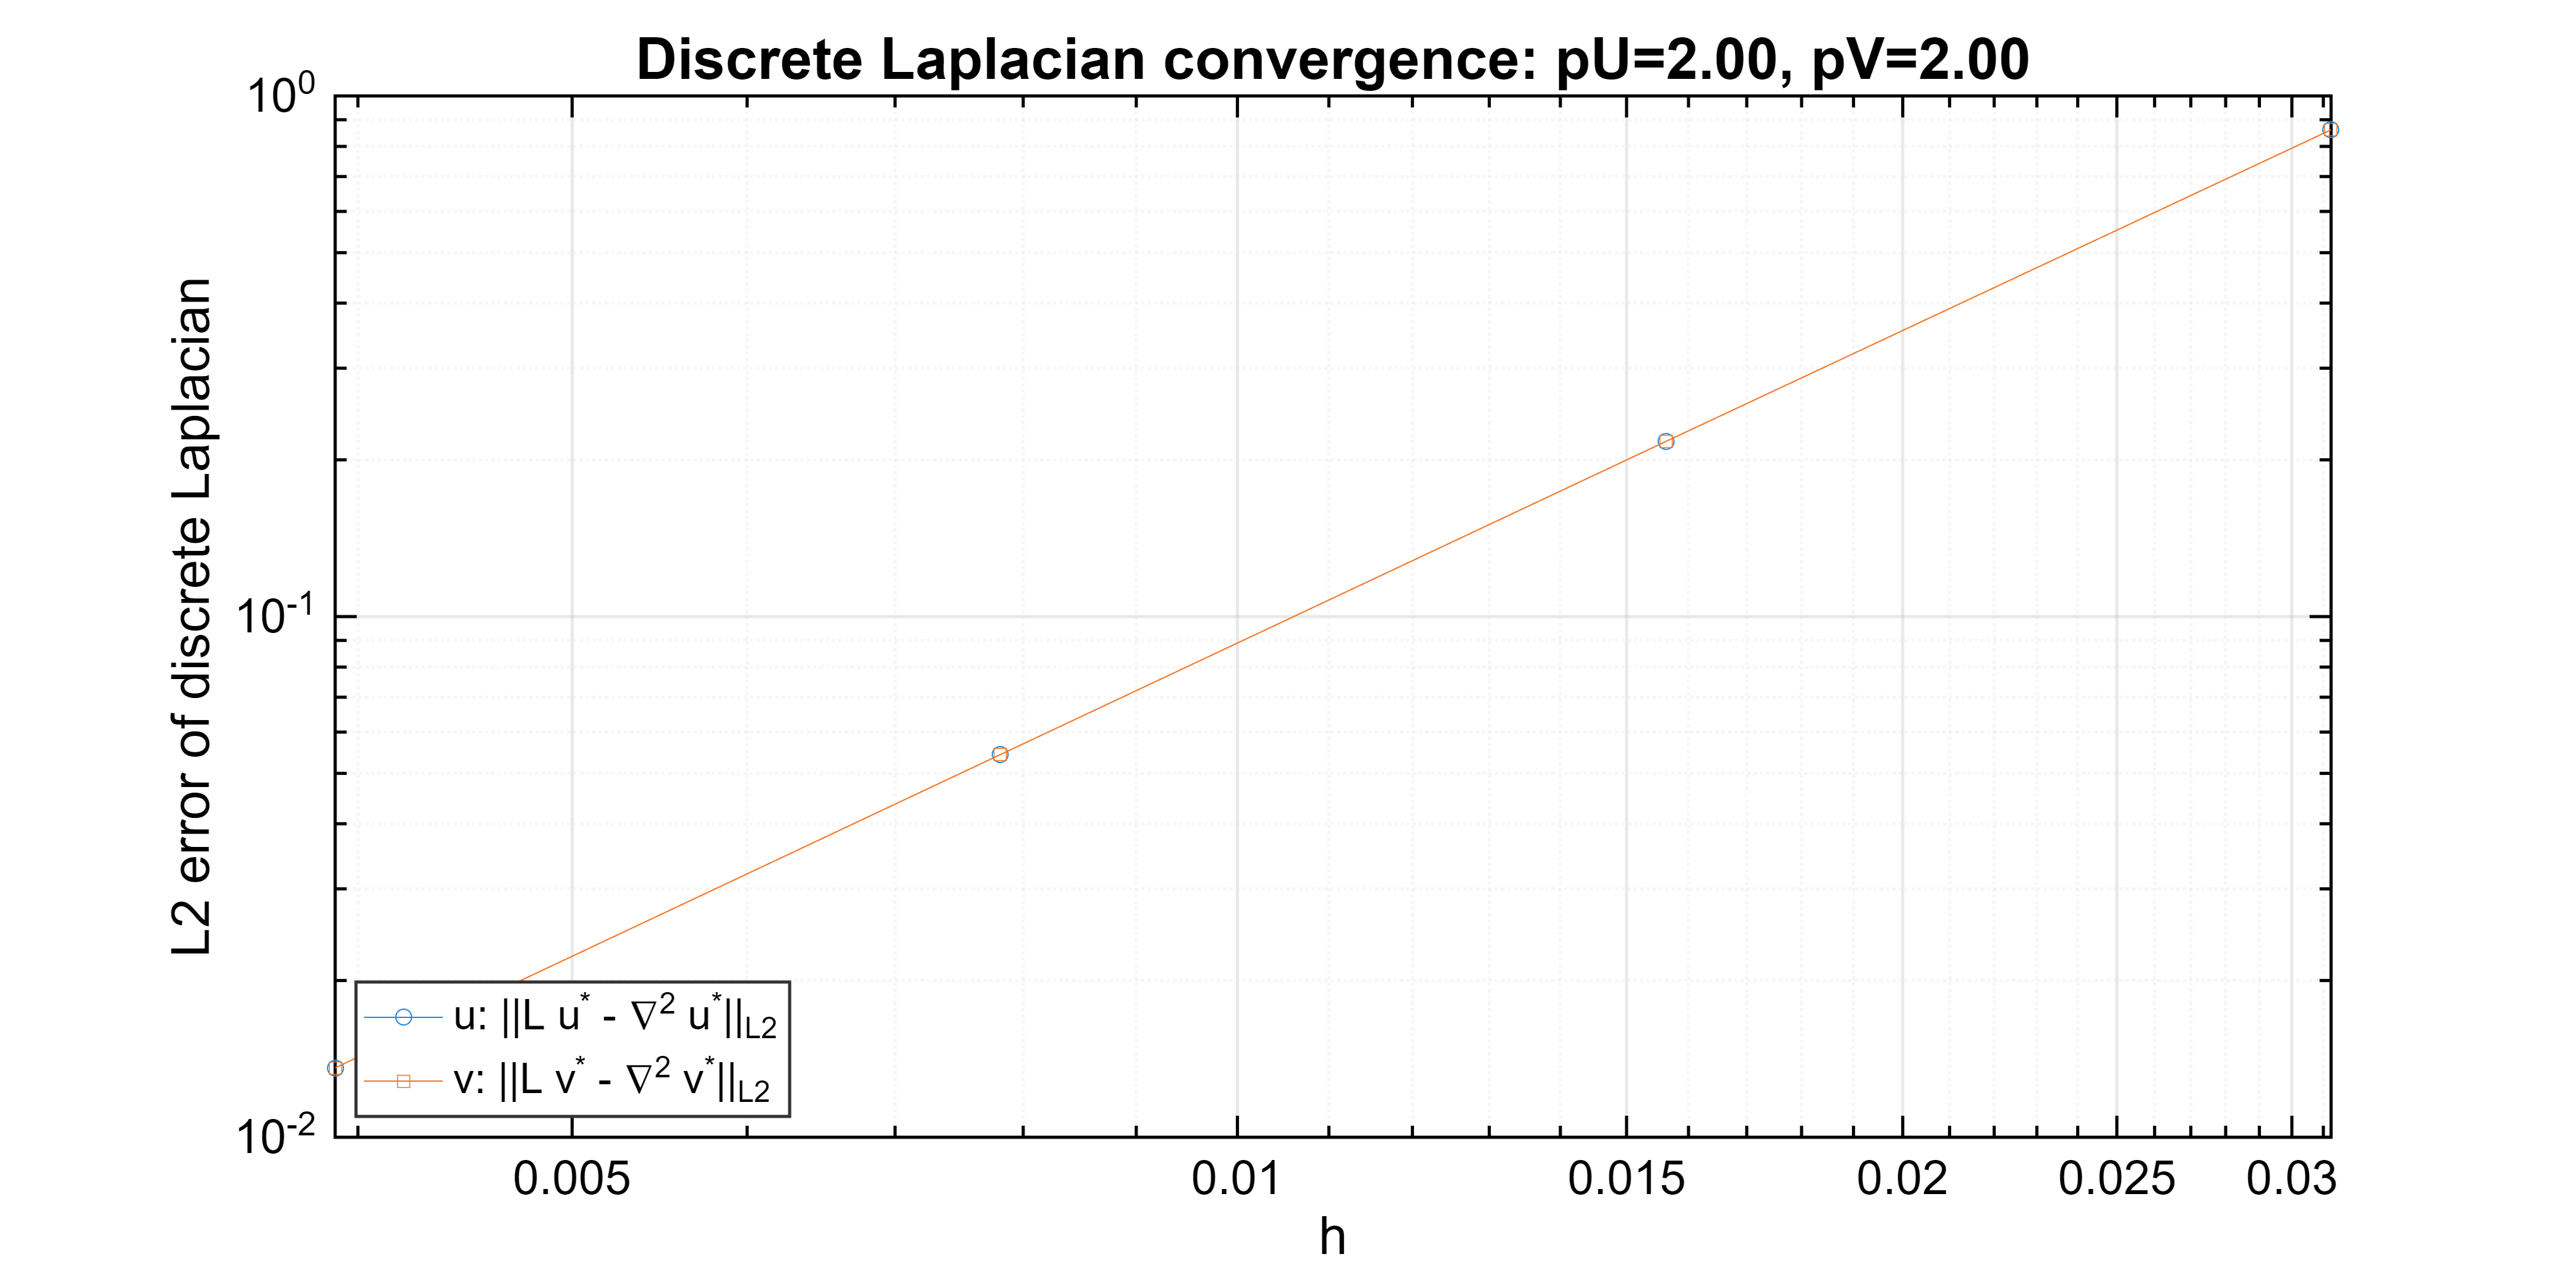
\includegraphics[width=0.82\textwidth]{figures/verification/mms_operator_convergence.png}
\caption{Log--log convergence plot for the discrete Laplacian MMS test.}
\label{fig:mms_operator_convergence}
\end{figure}

\subsection{Test Case 2: Temporal convergence of the explicit Euler scheme}
\label{sec:verification_testcase_timestep_convergence}

\paragraph{Aim.}
This test case verifies the temporal behavior of the explicit Euler time-integration scheme used in the Gray--Scott solver. Since explicit Euler is theoretically first-order accurate in time, the purpose of the test is to check whether the numerical solution shows the expected first-order convergence under time-step refinement while all spatial discretization settings are kept fixed.

\paragraph{Setup.}
The test is performed for the baseline Gray--Scott configuration on the square domain
\[
\Omega = [0,1)\times[0,1),
\]
using a uniform grid with
\[
N_x = N_y = 128.
\]
The model parameters are taken from \texttt{defaultParams()}:
\[
D_u = 2\times 10^{-5}, \qquad
D_v = 1\times 10^{-5}, \qquad
F = 0.03, \qquad
k = 0.06.
\]
Periodic boundary conditions are used on all sides. The final simulation time is
\[
T = 50.
\]

The initial condition is the standard baseline initialization used in the project: the field \(U\) is initialized close to \(1\), the field \(V\) close to \(0\), and a centered \(10\times 10\) square patch is imposed with
\[
U = 0.50, \qquad V = 0.25,
\]
followed by a small random perturbation with amplitude \(\texttt{icPerturb}=0.02\). In order to make the comparison reproducible, the random number generator is reset with the same seed before all runs, so that each simulation starts from exactly the same initial state.

The same problem is then solved three times with the matrix-based diffusion operator and with three different time-step sizes:
\[
\Delta t \in \{0.2,\;0.1,\;0.05\}.
\]
At the final time \(T\), the \(v\)-field of the three runs is compared. Since no exact time-dependent reference solution is used in this test, a self-convergence approach is applied through the successive differences
\[
d_{12} = \|v_{\Delta t} - v_{\Delta t/2}\|,
\qquad
d_{24} = \|v_{\Delta t/2} - v_{\Delta t/4}\|.
\]
These differences are evaluated in both the discrete \(L^2\)-norm and the discrete \(L^\infty\)-norm.

\paragraph{How to run the test case.}
From the project \texttt{tests} folder, run:
\begin{verbatim}
r = test_timestep_convergence();
\end{verbatim}

The test prints the measured successive differences and observed orders to the MATLAB command window and saves the generated figure in the local output folder of
\begin{verbatim}
tests/test_case_02_timestep_convergence/
\end{verbatim}

\paragraph{Expected result.}
For a first-order time-integration method, the temporal discretization error behaves as
\[
e(\Delta t) = C\,\Delta t + \mathcal{O}(\Delta t^2).
\]
Therefore, in the asymptotic regime, the successive-difference indicators are also expected to scale linearly with \(\Delta t\). In particular, halving the time step should approximately halve the difference, so that
\[
\frac{d_{12}}{d_{24}} \approx 2.
\]
The observed order estimate
\[
p = \frac{\log(d_{12}/d_{24})}{\log 2}
\]
should therefore be close to \(1\). In addition, the finer-step difference \(d_{24}\) should be smaller than the coarser-step difference \(d_{12}\).

\paragraph{Obtained result.}
The measured results are listed in Table~\ref{tab:timestep_convergence_data}, and the \(L^2\)-based refinement plot is shown in Fig.~\ref{fig:timestep_convergence}. The numerical results are
\[
d_{12}^{L^2} = 3.706\times 10^{-5}, \qquad
d_{24}^{L^2} = 1.851\times 10^{-5}, \qquad
p_{L^2} = 1.001,
\]
and
\[
d_{12}^{L^\infty} = 5.798\times 10^{-4}, \qquad
d_{24}^{L^\infty} = 2.891\times 10^{-4}, \qquad
p_{L^\infty} = 1.004.
\]

\begin{table}[htbp]
\centering
\caption{Measured successive differences and observed orders for the explicit Euler time-step refinement test.}
\label{tab:timestep_convergence_data}
\begin{tabular}{|c|c|c|c|}
\hline
Norm & \(d_{12}\) & \(d_{24}\) & Observed order \(p\) \\
\hline
\(L^2\)      & \(3.706\times 10^{-5}\) & \(1.851\times 10^{-5}\) & 1.001 \\
\(L^\infty\) & \(5.798\times 10^{-4}\) & \(2.891\times 10^{-4}\) & 1.004 \\
\hline
\end{tabular}
\end{table}

The finer-step difference is smaller than the coarser-step difference in both norms, as expected:
\[
d_{24}^{L^2} < d_{12}^{L^2},
\qquad
d_{24}^{L^\infty} < d_{12}^{L^\infty}.
\]
Moreover, the ratio between successive differences is essentially \(2\), which yields an observed order of approximately \(1\) in both norms. This is in excellent agreement with the theoretical first-order accuracy of the explicit Euler method.

Therefore, the test confirms that the implemented time-integration scheme behaves correctly under time-step refinement and that the solver is operating in the expected temporal convergence regime for this problem configuration.

\begin{figure}[htbp]
\centering
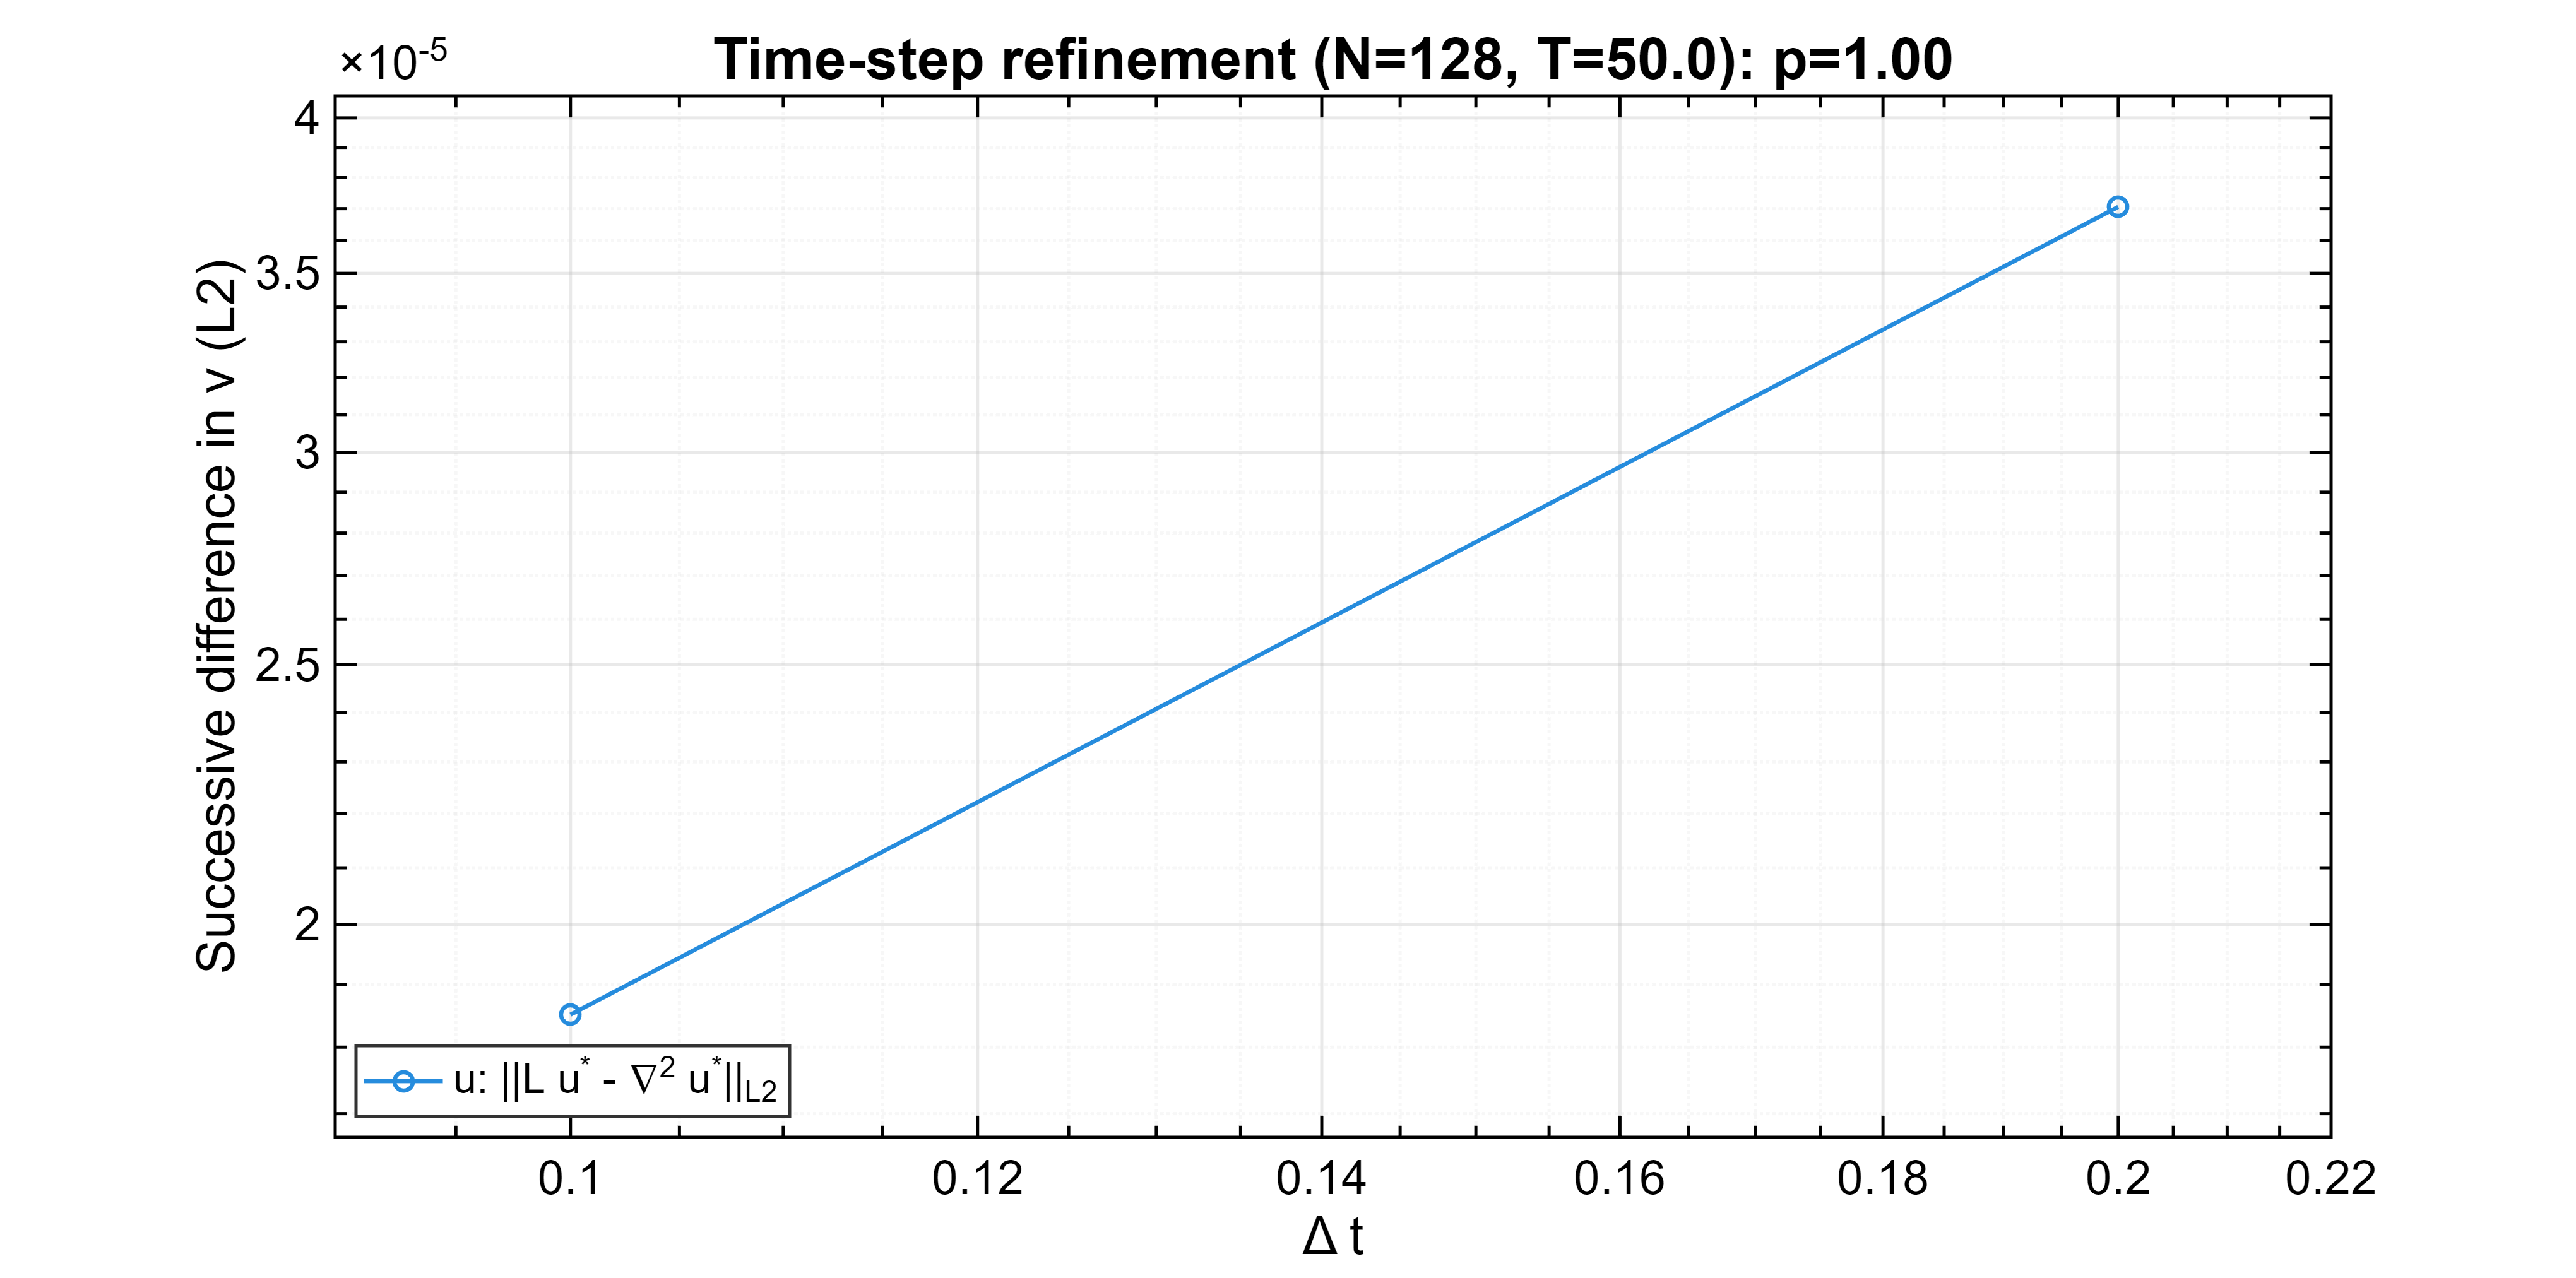
\includegraphics[width=0.82\textwidth]{figures/verification/timestep_convergence.png}
\caption{Time-step refinement test for the explicit Euler scheme. The plot shows the \(L^2\)-based successive differences of the \(v\)-field for \(\Delta t=0.2\) and \(\Delta t=0.1\), indicating first-order temporal convergence.}
\label{fig:timestep_convergence}
\end{figure}


\subsection{Test Case 3: Verification of boundary-condition enforcement}
\label{sec:verification_testcase_boundary_conditions}

\paragraph{Aim.}
This test case verifies that the implemented boundary-condition treatment is applied correctly and robustly in the Gray--Scott solver. Since support for non-periodic boundaries is an explicit feature of the project, it is important to check not only that Dirichlet and Neumann conditions are imposed correctly at the boundary nodes, but also that this enforcement remains stable during time integration and is consistent across all implemented diffusion modes.

\paragraph{Setup.}
The test is performed on the square domain
\[
\Omega = [0,1)\times[0,1)
\]
using a uniform grid with
\[
N_x=N_y=64.
\]
The time step is
\[
\Delta t = 0.25,
\]
and the test is repeated for all three diffusion implementations:
\[
\texttt{matrix}, \qquad \texttt{stencil}, \qquad \texttt{full}.
\]

The verification script combines three sub-checks within one test case.

\medskip
\noindent
\textbf{(1) Dirichlet constant enforcement.}
A smooth nontrivial initial field is prescribed for both species,
\[
U_0(x,y)=0.80+0.10\sin(2\pi x)\cos(2\pi y),
\]
\[
V_0(x,y)=0.20+0.05\cos(2\pi x)\sin(2\pi y),
\]
and a constant Dirichlet condition is imposed on the left boundary:
\[
u = 0.123, \qquad v = 0.456.
\]
The other three boundaries remain periodic. The simulation is advanced for 20 time steps, and after each step the maximum deviation of the left boundary values from the prescribed constants is recorded.

\medskip
\noindent
\textbf{(2) Neumann derivative consistency.}
The same smooth initial fields are used again, but now a constant Neumann condition is prescribed on the left boundary:
\[
\frac{\partial u}{\partial n}=1.0, \qquad \frac{\partial v}{\partial n}=-2.0.
\]
The other boundaries remain periodic. The run is again advanced for 20 time steps. After each step, the normal derivative at the left boundary is approximated by the discrete one-sided difference
\[
\frac{U(:,2)-U(:,1)}{h_x}, \qquad \frac{V(:,2)-V(:,1)}{h_x},
\]
and the maximum deviation from the prescribed derivative values is recorded.

\medskip
\noindent
\textbf{(3) Mixed boundary-condition robustness test.}
A more demanding long-time test is then performed with a strongly mismatched initial state,
\[
U_0 = 0.95, \qquad V_0 = 0.05
\]
throughout the interior, while the following boundary conditions are imposed:
\[
u=0.2,\quad v=0.4 \qquad \text{on the left boundary (Dirichlet)},
\]
\[
\frac{\partial u}{\partial n}=0,\quad \frac{\partial v}{\partial n}=0
\qquad \text{on the right boundary (Neumann)},
\]
with periodic boundaries at the top and bottom. This case is run for 400 time steps, corresponding to
\[
T = 100.
\]
During the run, the maximum boundary errors are tracked for both the Dirichlet and Neumann sides. In addition, an interior monitoring column is monitored in order to confirm that the solution evolves nontrivially in the interior and that the test is not merely a static boundary overwrite. The script also checks that no \texttt{NaN} or \texttt{Inf} values occur.

\paragraph{How to run the test case.}
From the project \texttt{tests} folder, run:
\begin{verbatim}
r = test_boundary_conditions();
\end{verbatim}

The test prints the maximum boundary errors for all three diffusion modes in the MATLAB command window.

\paragraph{Expected result.}
For the Dirichlet sub-test, the prescribed boundary values should be enforced exactly at every time step, up to machine precision. Therefore, the maximum boundary error should be essentially zero.

For the Neumann sub-test, the discrete boundary gradient should match the prescribed normal derivative. Since the condition is imposed directly in the discrete formulation, the resulting error should again be at the level of roundoff.

For the mixed long-time test, the left Dirichlet boundary should remain fixed at its prescribed values and the right Neumann boundary should remain zero-flux throughout the simulation. At the same time, the interior should evolve measurably away from the initial state. Thus, the expected result is:
\begin{itemize}
    \item boundary errors at or near machine precision,
    \item no \texttt{NaN} or \texttt{Inf} values,
    \item nonzero interior change,
    \item and identical qualitative behavior for \texttt{matrix}, \texttt{stencil}, and \texttt{full} modes.
\end{itemize}

\paragraph{Obtained result.}
All checks passed for all three diffusion modes. The returned test result was
\[
\texttt{pass} = 1,
\]
and the script reported that the quantitative Dirichlet, Neumann, and mixed boundary-condition checks passed for \texttt{matrix}, \texttt{stencil}, and \texttt{full} modes.

The measured results are summarized separately in Tables~\ref{tab:bc_dirichlet_verification}, \ref{tab:bc_neumann_verification}, and \ref{tab:bc_mixed_verification}. For the Dirichlet test, the maximum boundary error was exactly zero for both \(u\) and \(v\) in all three modes over 20 steps. For the Neumann test, the maximum error was zero for \(u\) and
\[
3.553\times 10^{-15}
\]
for \(v\), which is at the level of machine precision and therefore consistent with exact discrete enforcement up to floating-point roundoff.

In the mixed 400-step test, the maximum Dirichlet and Neumann boundary errors remained zero for both species in all three diffusion modes. At the same time, the interior change values changed by
\[
2.992\times 10^{-2} \quad \text{for } u,
\qquad
4.982\times 10^{-2} \quad \text{for } v,
\]
which confirms that the solution evolved nontrivially in the interior while the imposed boundary conditions remained exactly enforced.

The fact that the reported errors are identical for \texttt{matrix}, \texttt{stencil}, and \texttt{full} is a strong indication that the boundary-condition handling is implemented consistently across all diffusion formulations.

\begin{table}[htbp]
\centering
\caption{Dirichlet boundary-condition verification results for all diffusion modes.}
\label{tab:bc_dirichlet_verification}
\begin{tabular}{|c|c|c|}
\hline
Mode & maxErr \(u\) & maxErr \(v\) \\
\hline
\texttt{matrix}  & \(0.000\times 10^{0}\) & \(0.000\times 10^{0}\) \\
\texttt{stencil} & \(0.000\times 10^{0}\) & \(0.000\times 10^{0}\) \\
\texttt{full}    & \(0.000\times 10^{0}\) & \(0.000\times 10^{0}\) \\
\hline
\end{tabular}
\end{table}

\begin{table}[htbp]
\centering
\caption{Neumann boundary-condition verification results for all diffusion modes.}
\label{tab:bc_neumann_verification}
\begin{tabular}{|c|c|c|}
\hline
Mode & maxErr \(u\) & maxErr \(v\) \\
\hline
\texttt{matrix}  & \(0.000\times 10^{0}\) & \(3.553\times 10^{-15}\) \\
\texttt{stencil} & \(0.000\times 10^{0}\) & \(3.553\times 10^{-15}\) \\
\texttt{full}    & \(0.000\times 10^{0}\) & \(3.553\times 10^{-15}\) \\
\hline
\end{tabular}
\end{table}

\begin{table}[htbp]
\centering
\small
\setlength{\tabcolsep}{4pt}
\renewcommand{\arraystretch}{1.15}
\caption{Mixed boundary-condition robustness results for all diffusion modes after 400 steps.}
\label{tab:bc_mixed_verification}
\begin{tabular}{|c|c|c|c|c|c|c|}
\hline
Mode
& \shortstack{maxDir\\\(u\)}
& \shortstack{maxDir\\\(v\)}
& \shortstack{maxNeu\\\(u\)}
& \shortstack{maxNeu\\\(v\)}
& \shortstack{interior\\change \(\Delta u\)}
& \shortstack{interior\\change \(\Delta v\)} \\
\hline
\texttt{matrix}  & \(0.000\times 10^{0}\) & \(0.000\times 10^{0}\) & \(0.000\times 10^{0}\) & \(0.000\times 10^{0}\) & \(2.992\times 10^{-2}\) & \(4.982\times 10^{-2}\) \\
\texttt{stencil} & \(0.000\times 10^{0}\) & \(0.000\times 10^{0}\) & \(0.000\times 10^{0}\) & \(0.000\times 10^{0}\) & \(2.992\times 10^{-2}\) & \(4.982\times 10^{-2}\) \\
\texttt{full}    & \(0.000\times 10^{0}\) & \(0.000\times 10^{0}\) & \(0.000\times 10^{0}\) & \(0.000\times 10^{0}\) & \(2.992\times 10^{-2}\) & \(4.982\times 10^{-2}\) \\
\hline
\end{tabular}
\end{table}

Overall, this test case confirms that the boundary-condition treatment is not only mathematically correct at the discrete level, but also numerically robust during time stepping and consistent across all solver variants used in the project.


\subsection{Test Case 4: Matrix--stencil equivalence of the diffusion operator}
\label{sec:verification_testcase_laplacian_equivalence}

\paragraph{Aim.}
This test case verifies that the two implemented diffusion-operator realizations, namely the sparse matrix formulation and the matrix-free stencil formulation, produce the same numerical result when applied to the same discrete field. Since both implementations are intended to represent the same five-point finite-difference Laplacian on a periodic grid, this test is an important consistency check at the operator level.

\paragraph{Setup.}
The test compares the output of the sparse matrix Laplacian assembled by \texttt{buildLaplacian2D} with the output of the matrix-free stencil operator evaluated by \texttt{applyLaplacianStencil}. The comparison is carried out for periodic connectivity only, because physical boundary conditions such as Dirichlet and Neumann are imposed separately after each time step and are therefore not part of this operator-equivalence test.

Three different grid sizes are used in order to detect possible indexing, reshaping, or dimension-ordering mistakes:
\[
32\times 32,\qquad 64\times 48,\qquad 128\times 128.
\]
For each grid, three independent random trials are performed. In each trial, a random discrete field \(u\) is generated, and the following two operator evaluations are computed:
\[
a = Lu,
\qquad
b = \mathcal{S}(u),
\]
where \(L\) denotes the sparse matrix Laplacian and \(\mathcal{S}\) denotes the stencil-based Laplacian application.

The difference between the two results is measured using:
\[
\text{relative error} = \frac{\|a-b\|_2}{\max(1,\|a\|_2)},
\]
and
\[
\text{maximum absolute difference} = \max_i |a_i-b_i|.
\]

The tolerances used by the test are
\[
\texttt{relTol} = 10^{-12},
\qquad
\texttt{absTol} = 10^{-10}.
\]

\paragraph{How to run the test case.}
From the project \texttt{tests} folder, run:
\begin{verbatim}
r = test_laplacian_stencil_equivalence();
\end{verbatim}

The test prints the relative and absolute differences for each grid and trial and reports the worst observed case.

\paragraph{Expected result.}
Both implementations represent the same discrete Laplacian operator. Therefore, for the same input vector \(u\), their outputs should agree up to floating-point roundoff. As a result, the relative error should be extremely small, and the maximum absolute difference should remain below the prescribed numerical tolerances. In particular, all trials should pass with margins far below
\[
10^{-12}\quad \text{(relative)}
\qquad\text{and}\qquad
10^{-10}\quad \text{(absolute)}.
\]

\paragraph{Obtained result.}
All nine test cases passed successfully, and the returned result was
\[
\texttt{pass} = 1.
\]
The measured values are listed in Table~\ref{tab:matrix_stencil_operator_equivalence}. The relative errors were consistently on the order of \(10^{-16}\), which is close to machine precision. The largest observed relative error was
\[
1.249\times 10^{-16}
\]
for the \(64\times 48\) grid in trial 2. The largest observed maximum absolute difference was
\[
5.821\times 10^{-11}
\]
for the \(128\times 128\) grid in trial 1.

These worst-case values are still safely below the prescribed tolerances:
\[
1.249\times 10^{-16} \ll 10^{-12},
\qquad
5.821\times 10^{-11} < 10^{-10}.
\]
The slightly larger absolute differences on the finest grid are expected because larger systems may accumulate somewhat more floating-point roundoff, but the differences remain numerically negligible.

Therefore, the test confirms that the matrix-based and stencil-based diffusion operators are equivalent to machine precision and can be regarded as two consistent implementations of the same finite-difference Laplacian.

\begin{table}[htbp]
\centering
\caption{Matrix--stencil operator equivalence results for all tested grids and trials.}
\label{tab:matrix_stencil_operator_equivalence}
\begin{tabular}{|c|c|c|c|}
\hline
Grid & Trial & Relative error & Max absolute difference \\
\hline
\(32\times 32\)   & 1 & \(1.145\times 10^{-16}\) & \(3.638\times 10^{-12}\) \\
\(32\times 32\)   & 2 & \(1.127\times 10^{-16}\) & \(1.819\times 10^{-12}\) \\
\(32\times 32\)   & 3 & \(1.132\times 10^{-16}\) & \(1.819\times 10^{-12}\) \\
\(64\times 48\)   & 1 & \(1.211\times 10^{-16}\) & \(7.276\times 10^{-12}\) \\
\(64\times 48\)   & 2 & \(1.249\times 10^{-16}\) & \(1.455\times 10^{-11}\) \\
\(64\times 48\)   & 3 & \(1.181\times 10^{-16}\) & \(7.276\times 10^{-12}\) \\
\(128\times 128\) & 1 & \(1.131\times 10^{-16}\) & \(5.821\times 10^{-11}\) \\
\(128\times 128\) & 2 & \(1.132\times 10^{-16}\) & \(5.821\times 10^{-11}\) \\
\(128\times 128\) & 3 & \(1.118\times 10^{-16}\) & \(5.821\times 10^{-11}\) \\
\hline
\end{tabular}
\end{table}


\subsection{Test Case 5: End-to-end equivalence of matrix and stencil solver modes}
\label{sec:verification_testcase_solver_equivalence}

\paragraph{Aim.}
This test case verifies that the matrix-based and stencil-based diffusion modes are equivalent at the level of the full Gray--Scott simulation, not only at the isolated operator level. In contrast to the previous operator-equivalence test, this case checks the complete solver workflow, including model initialization, time stepping, reaction evaluation, diffusion application, and state updates. Its purpose is to confirm that both solver modes produce the same final numerical solution when they are run with identical settings.

\paragraph{Setup.}
The test uses the full \texttt{GrayScottModel} class on the square periodic domain
\[
\Omega = [0,1)\times[0,1),
\]
with a uniform grid
\[
N_x = N_y = 128.
\]
The standard project parameters from \texttt{defaultParams()} are used:
\[
D_u = 2\times 10^{-5}, \qquad
D_v = 1\times 10^{-5}, \qquad
F = 0.03, \qquad
k = 0.06.
\]
The time step is
\[
\Delta t = 0.2,
\]
and the final simulation time is
\[
T = 5.
\]

Two runs are then carried out:

\begin{itemize}
    \item a baseline run with \texttt{diffusionMode = "matrix"},
    \item a comparison run with \texttt{diffusionMode = "stencil"}.
\end{itemize}

To ensure that both runs start from exactly the same initial condition, the random number generator is reset to the same seed before each run. The same grid and the same model parameters are used in both cases. After both simulations reach the final time \(T\), the final states are compared componentwise.

Let \(u_A, v_A\) denote the final matrix-mode solution and \(u_B, v_B\) the final stencil-mode solution. The test evaluates the differences
\[
d_u = u_A - u_B, \qquad d_v = v_A - v_B,
\]
and computes both relative and maximum absolute differences:
\[
\mathrm{rel}_u = \frac{\|d_u\|_2}{\max(1,\|u_A\|_2)}, \qquad
\mathrm{rel}_v = \frac{\|d_v\|_2}{\max(1,\|v_A\|_2)},
\]
\[
\mathrm{max}_u = \max_i |d_{u,i}|, \qquad
\mathrm{max}_v = \max_i |d_{v,i}|.
\]

The tolerances used by the test are
\[
\texttt{relTol} = 10^{-10}, \qquad
\texttt{absTol} = 10^{-9}.
\]

\paragraph{How to run the test case.}
From the project \texttt{tests} folder, run:
\begin{verbatim}
r = test_matrix_stencil_endtoend_equivalence();
\end{verbatim}

The test prints the measured relative and maximum absolute differences in the MATLAB command window.

\paragraph{Expected result.}
If the matrix-based and stencil-based diffusion modes are truly equivalent implementations of the same numerical method, then the complete Gray--Scott runs should produce the same final solution up to floating-point roundoff. Therefore, the relative differences in both \(u\) and \(v\) should be extremely small, and the maximum absolute differences should remain far below the prescribed tolerances. In particular, both solution components should satisfy
\[
\mathrm{rel}_u < 10^{-10}, \qquad \mathrm{rel}_v < 10^{-10},
\]
and
\[
\mathrm{max}_u < 10^{-9}, \qquad \mathrm{max}_v < 10^{-9}.
\]

\paragraph{Obtained result.}
The test passed successfully, and the returned result was
\[
\texttt{pass} = 1.
\]
The measured final-state differences are summarized in Table~\ref{tab:matrix_stencil_endtoend_equivalence}.

\begin{table}[htbp]
\centering
\caption{End-to-end comparison between matrix and stencil solver modes at final time \(T=5\).}
\label{tab:matrix_stencil_endtoend_equivalence}
\begin{tabular}{|c|c|}
\hline
Quantity & Measured value \\
\hline
\(\mathrm{rel}_u\) & \(8.903\times 10^{-17}\) \\
\(\mathrm{rel}_v\) & \(9.927\times 10^{-17}\) \\
\(\mathrm{max}_u\) & \(4.441\times 10^{-16}\) \\
\(\mathrm{max}_v\) & \(5.551\times 10^{-17}\) \\
\hline
\end{tabular}
\end{table}

All reported differences are many orders of magnitude smaller than the specified tolerances:
\[
8.903\times 10^{-17} \ll 10^{-10}, \qquad
9.927\times 10^{-17} \ll 10^{-10},
\]
\[
4.441\times 10^{-16} \ll 10^{-9}, \qquad
5.551\times 10^{-17} \ll 10^{-9}.
\]
Thus, the final solutions produced by the two solver modes are numerically indistinguishable up to machine precision.

This result shows that the stencil-based and matrix-based implementations remain consistent not only when applying the Laplacian to a test vector, but also when embedded in the full Gray--Scott time integration process.


\subsection{Test Case 6: GUI and non-GUI consistency}
\label{sec:verification_testcase_gui_consistency}

\paragraph{Aim.}
This test case verifies that the graphical user interface does not alter the numerical model and that a simulation executed through the GUI reproduces exactly the same numerical results as the corresponding non-GUI workflow. The purpose is to check consistency at the interface level, i.e.\ to confirm that the GUI acts only as a control and visualization layer and does not introduce unintended changes in parameters, initialization, or solver behavior.

\paragraph{Setup.}
The consistency check is carried out in three stages. First, a non-GUI reference run is generated using the same parameter set as the GUI startup configuration. Second, the GUI is launched with its current shipped default setup and a dedicated helper script advances the GUI-owned model for the exact number of required time steps. Third, the saved non-GUI and GUI results are compared quantitatively.

For the run documented here, the GUI startup configuration was:
\[
\texttt{preset}=\texttt{pearson}, \qquad
\texttt{diffusionMode}=\texttt{stencil},
\]
with periodic boundary conditions on all sides. The computational grid was
\[
N_x = N_y = 256,
\]
the time step was
\[
\Delta t = 0.5,
\]
and the final simulation time was
\[
T = 500.
\]
Therefore, the total number of time steps was
\[
n_{\text{steps}} = \frac{T}{\Delta t} = \frac{500}{0.5} = 1000.
\]
A midpoint snapshot was stored at
\[
k_{\text{snap}} = 500.
\]

The comparison includes both the midpoint snapshot and the final state for the two species \(u\) and \(v\). For each compared field, the following quantities are evaluated:
\[
\mathrm{relL2} = \frac{\|w_{\mathrm{GUI}} - w_{\mathrm{ref}}\|_2}{\max(1,\|w_{\mathrm{ref}}\|_2)},
\qquad
\mathrm{maxAbs} = \max_i |w_{\mathrm{GUI},i} - w_{\mathrm{ref},i}|.
\]
The tolerances used by the comparison script are
\[
\texttt{tol\_relL2} = 10^{-12},
\qquad
\texttt{tol\_maxAbs} = 10^{-12}.
\]

The relevant scripts are:
\begin{verbatim}
run_nongui_reference_dump.m
run_gui_consistency_dump.m
compare_gui_nongui.m
\end{verbatim}

All three files are located in:
\begin{verbatim}
tests/test_case_06_gui_nongui_consistency/
\end{verbatim}

\paragraph{How to run the test case.}
Run the workflow either from the project root or from
\texttt{tests/test\_case\_06\_gui\_nongui\_consistency}. Make sure that the project paths are available. Then execute:
\begin{verbatim}
ref = run_nongui_reference_dump();
gui = run_gui_consistency_dump();
T   = compare_gui_nongui(ref.refFile, gui.guiFile);
\end{verbatim}

The first two helper scripts save their generated \texttt{.mat} files in the local output folder of
\texttt{tests/test\_case\_06\_gui\_nongui\_consistency/}. The comparison script can read those files directly when their paths are passed explicitly, as shown above. If \texttt{compare\_gui\_nongui()} is called without arguments, it instead searches for comparison input files in the local \texttt{inputs/} folder.

For the documented run, the workflow produced the non-GUI dump, the GUI dump, the comparison CSV file, and the comparison figure in the local output folder
\begin{verbatim}
tests/test_case_06_gui_nongui_consistency/
\end{verbatim}

\paragraph{Expected result.}
If the GUI is consistent with the underlying solver implementation, then the GUI-generated run and the non-GUI reference run should produce identical or numerically indistinguishable data when started from the same configuration. Since this test uses the same model parameters, same grid, same seed, same number of steps, and the same solver configuration, the expected result is that both the midpoint snapshot and the final state match within the very strict tolerances
\[
10^{-12}
\]
for both the relative \(L^2\) difference and the maximum absolute difference.

\paragraph{Obtained result.}
The comparison passed in all four checked cases: snapshot \(u\), snapshot \(v\), final \(u\), and final \(v\). The measured results are summarized in Table~\ref{tab:gui_nongui_consistency}. In every case,
\[
\mathrm{relL2} = 0,
\qquad
\mathrm{maxAbs} = 0,
\]
and the pass flag was \texttt{true}. Therefore, the GUI and non-GUI workflows produced exactly identical saved states for both the midpoint snapshot and the final solution.

\begin{table}[htbp]
\centering
\caption{GUI and non-GUI consistency comparison results.}
\label{tab:gui_nongui_consistency}
\begin{tabular}{|c|c|c|c|c|}
\hline
Stage & Field & relL2 & maxAbs & Pass \\
\hline
snapshot & \(u\) & 0 & 0 & true \\
snapshot & \(v\) & 0 & 0 & true \\
final    & \(u\) & 0 & 0 & true \\
final    & \(v\) & 0 & 0 & true \\
\hline
\end{tabular}
\end{table}

Figure~\ref{fig:gui_nongui_consistency} shows the GUI--non-GUI difference field for the snapshot of \(u\). The plotted field is identically zero, which is fully consistent with the tabulated comparison metrics. The same conclusion applies to the other compared states as well.

Hence, this test confirms that the GUI layer does not modify the mathematical or numerical behavior of the solver. It reproduces the same results as the non-GUI reference workflow exactly for the tested configuration.

\begin{figure}[htbp]
\centering
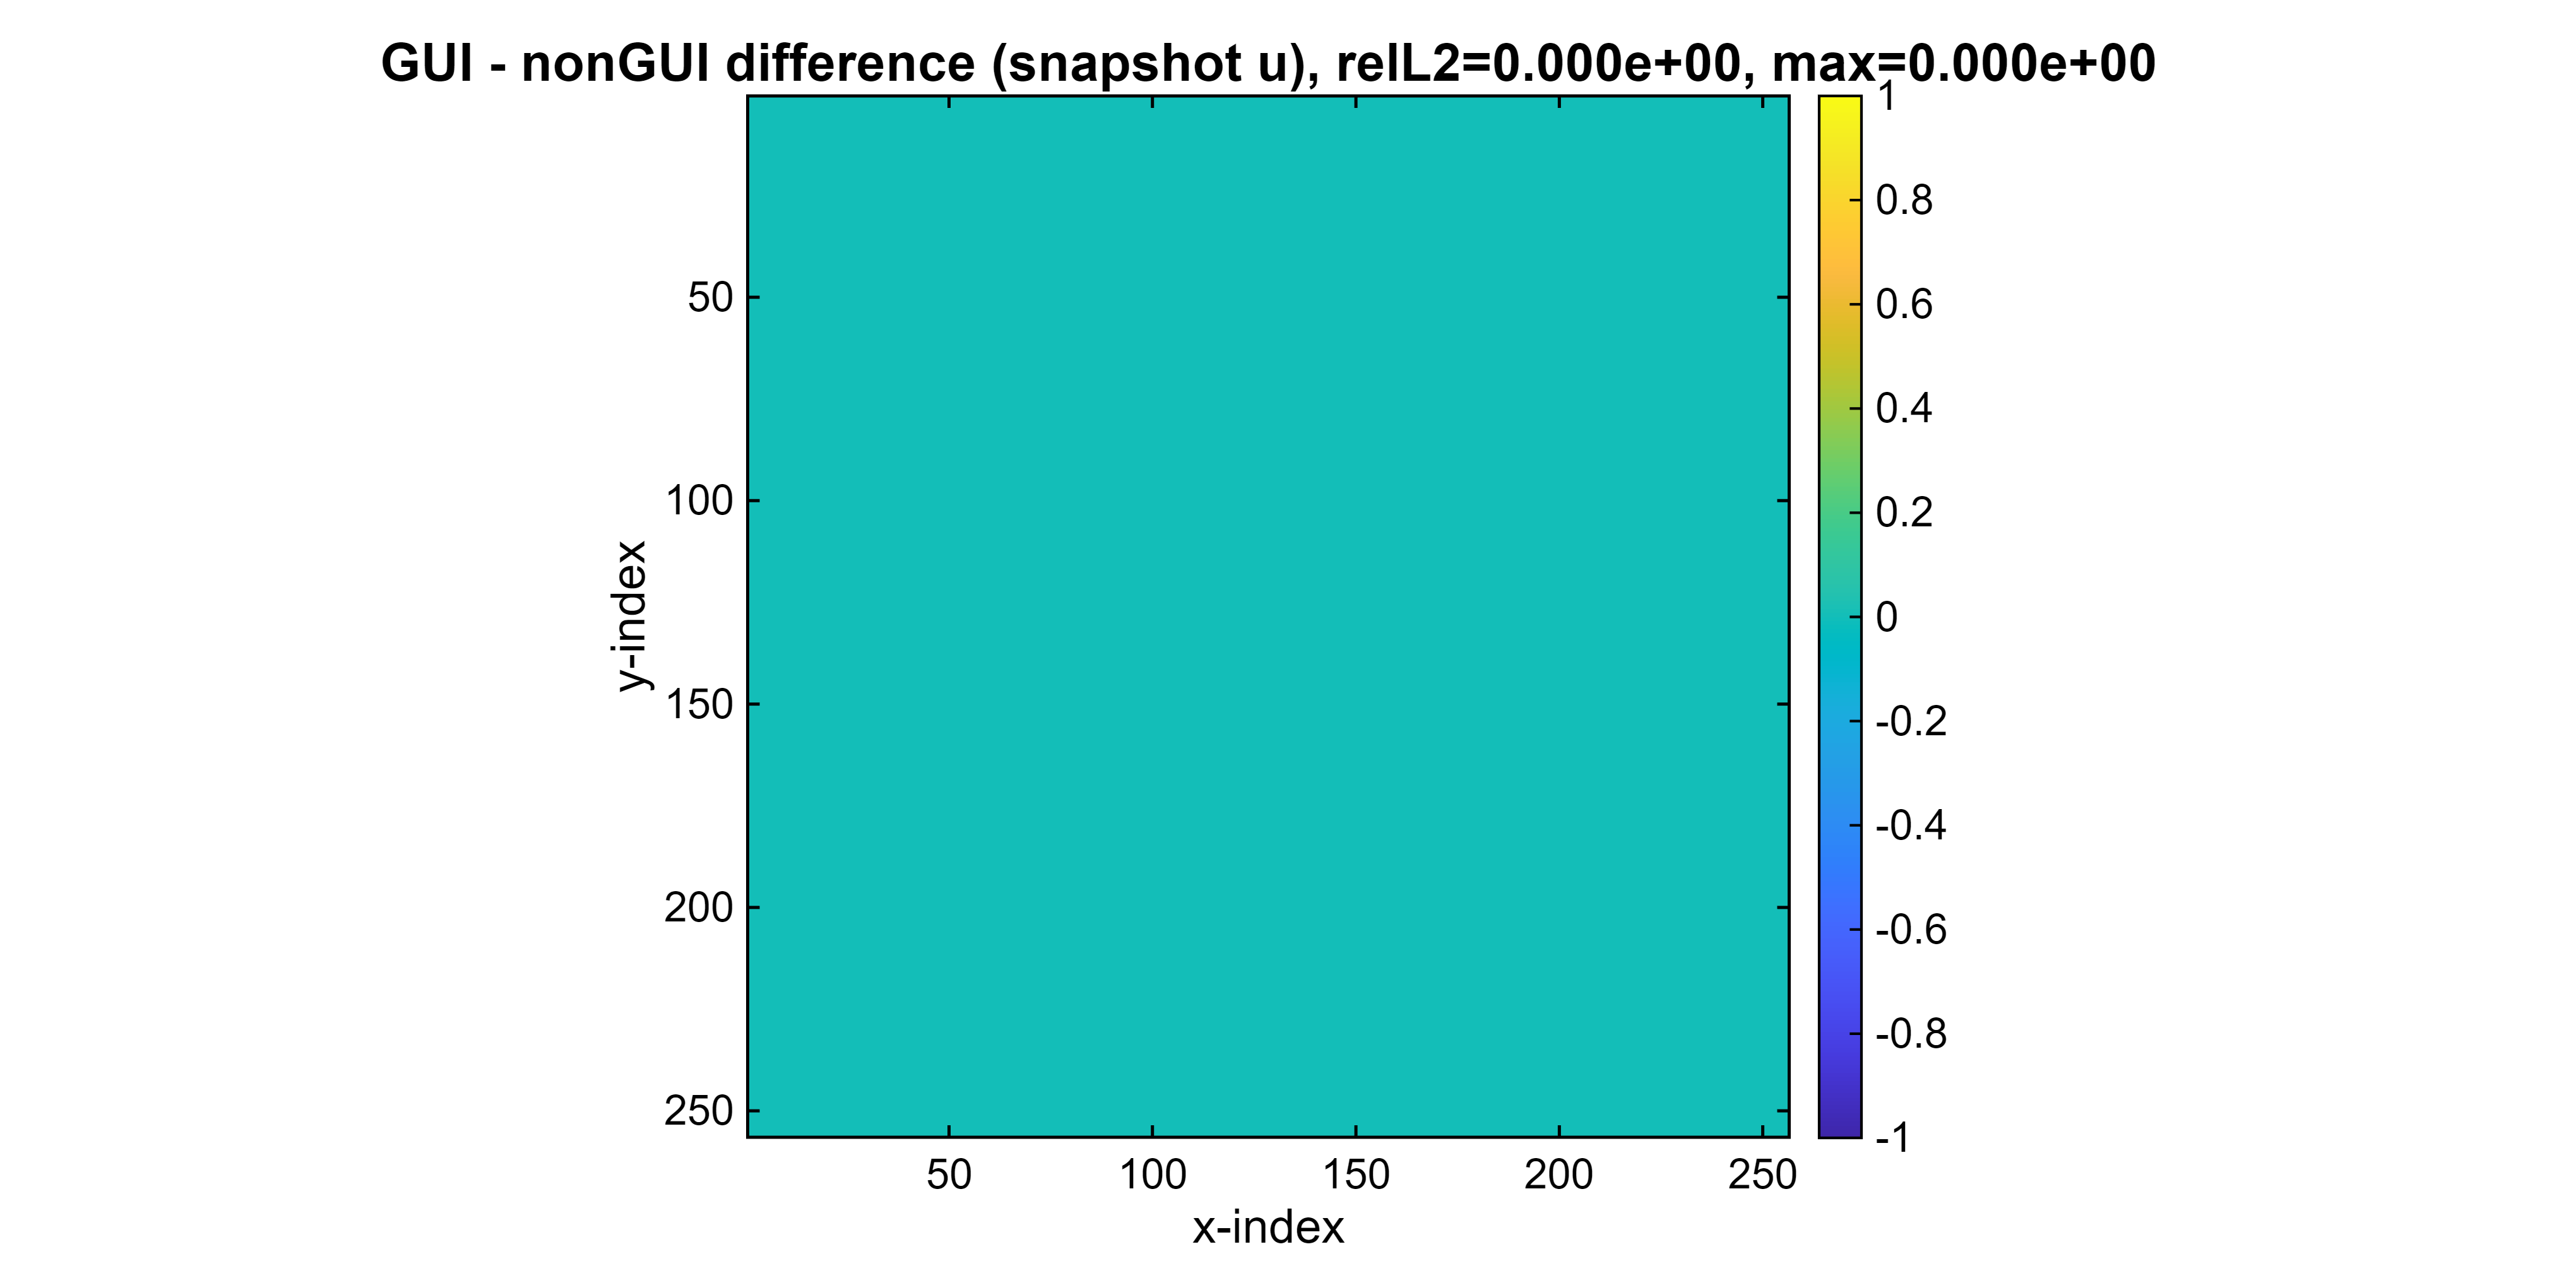
\includegraphics[width=0.78\textwidth]{figures/verification/gui_consistency.png}
\caption{Difference field between GUI and non-GUI results for the snapshot of \(u\). The field is identically zero, confirming exact agreement for the documented run.}
\label{fig:gui_nongui_consistency}
\end{figure}

\subsection{Test Case 7: Gray--Scott grid refinement test}
\label{sec:verification_testcase_grid_refinement}

\paragraph{Aim.}
This test case investigates how the numerical solution of the full nonlinear Gray--Scott system changes under spatial grid refinement. Unlike the manufactured-solution tests, this is not an exact-solution verification test, because no analytical reference solution is available for the pattern-forming nonlinear problem considered here. The goal is therefore more practical: to check whether the computed solution approaches a sufficiently fine-grid reference in a systematic way as the mesh is refined, and whether the observed behavior is consistent with the expected second-order spatial discretization used in the solver.

\paragraph{Initial idea and first difficulty.}
The original idea of this test was straightforward. The Gray--Scott system was solved on a sequence of grids, the finest grid was used as a numerical reference, and the coarser-grid solutions were compared against that reference in the discrete \(L^2\) norm. The time step was scaled as \(\Delta t \sim h^2\) in order to reduce the influence of the first-order explicit Euler time discretization and make the comparison mainly sensitive to spatial effects.

However, the first version of the test did not give the expected result. Although the errors decreased monotonically under refinement, the observed rates remained noticeably below the ideal value \(2\). At first sight, this could suggest that the fully nonlinear Gray--Scott dynamics, especially the phase-sensitive pattern evolution, prevented a clean refinement study. A closer inspection showed that this was only part of the explanation.

\paragraph{Why the first version was not fully reliable.}
The main issue in the original version was that the initialization was not grid-independent. The standard Gray--Scott pattern-seeding setup used in the project is suitable for normal simulations, but it is not ideal for a formal refinement study. In particular, the original initialization contained two features that made the comparison across grids less clean:

\begin{enumerate}
    \item The initial square perturbation was prescribed in a fixed number of grid cells rather than in physical coordinates. As a result, its physical size changed when the grid was refined.
    \item A random perturbation was added independently on each grid. Even with the same random seed, this does not represent the same physical perturbation sampled on different meshes.
\end{enumerate}

Therefore, the different grid levels did not correspond to exactly the same initial-value problem. For a nonlinear pattern-forming PDE such as the Gray--Scott system, even small differences in the initial condition can later produce visible phase shifts, slight pattern displacements, and morphology changes. Consequently, the discrete \(L^2\) difference between two solutions may reflect not only discretization error, but also mismatch in the underlying evolving pattern.

This analysis explained why the original version produced only moderate observed rates even though the error still decreased consistently.

\paragraph{Correction of the test design.}
To make the refinement study meaningful, the test was reformulated so that all grid levels solve the same problem as closely as possible. Two changes were introduced:

\begin{enumerate}
    \item The original grid-dependent seeded pattern was replaced by a smooth Gaussian-type initial condition defined directly in physical coordinates.
    \item The random perturbation was disabled for this test.
\end{enumerate}

With these two changes, every grid represents the same smooth initial state sampled at different resolutions. This removes the main inconsistency of the original setup and makes the subsequent comparison much more suitable for measuring refinement behavior.

In addition, the final simulation time was reduced to
\[
T = 0.2,
\]
instead of using a longer pattern-development time. This makes the test less sensitive to long-time nonlinear phase drift and allows the spatial discretization error to remain the dominant effect.

\paragraph{Final setup used for the reported result.}
The corrected test was carried out for the Gray--Scott model on the periodic square domain
\[
\Omega = [0,1)\times[0,1)
\]
with the baseline parameter set
\[
D_u = 2\times 10^{-5}, \qquad
D_v = 1\times 10^{-5}, \qquad
F = 0.03, \qquad
k = 0.06.
\]
The problem was solved on the sequence of uniform grids
\[
N_x=N_y \in \{64,\,128,\,256,\,512,\,1024,\,2048\}.
\]
The finest grid,
\[
N_x=N_y=2048,
\]
was used as the numerical reference solution. The reference fields were interpolated onto the coarser grids using cubic interpolation before computing the discrete \(L^2\) differences.

The time step was again scaled as
\[
\Delta t \sim h^2,
\]
with
\[
\Delta t = 0.01 \quad \text{for } N=64,
\]
and then reduced by a factor of four whenever the grid spacing was halved. This gives
\[
\Delta t \in \left\{
0.01,\;
0.0025,\;
0.000625,\;
0.00015625,\;
3.90625\times 10^{-5},\;
9.765625\times 10^{-6}
\right\}.
\]
The corresponding numbers of time steps are
\[
N_t \in \{20,\;80,\;320,\;1280,\;5120,\;20480\},
\]
after adjusting \(\Delta t\) slightly so that \(T/\Delta t\) is an integer in each case.

For each coarse grid, the discrete \(L^2\) differences were computed as
\[
e_U = \|U_h - U_{\mathrm{ref}}\|_{L^2}, \qquad
e_V = \|V_h - V_{\mathrm{ref}}\|_{L^2},
\]
and the observed refinement rates \(p_U\) and \(p_V\) were estimated from the log--log slope of error versus grid spacing.

\paragraph{How to run the test case.}
From the project \texttt{tests} folder, run:
\begin{verbatim}
r = test_grayscott_grid_refinement();
\end{verbatim}

The test executes all grid levels, interpolates the finest-grid reference onto the coarser meshes, reports the measured \(L^2\) differences, and saves the refinement plot in the local output folder of
\begin{verbatim}
tests/test_case_07_grayscott_grid_refinement/
\end{verbatim}

\paragraph{Obtained result.}
With the corrected grid-independent initialization, the test produced a much cleaner refinement trend than the original version. The returned test result was
\[
\texttt{pass} = 1.
\]

The measured \(L^2\) differences are given in Table~\ref{tab:grayscott_grid_refinement}. For both \(U\) and \(V\), the error decreases monotonically over all grid levels:
\[
4.522\times 10^{-7}
\rightarrow
1.133\times 10^{-7}
\rightarrow
2.802\times 10^{-8}
\rightarrow
6.674\times 10^{-9}
\rightarrow
1.335\times 10^{-9}
\]
for \(U\), and
\[
9.872\times 10^{-8}
\rightarrow
2.474\times 10^{-8}
\rightarrow
6.120\times 10^{-9}
\rightarrow
1.458\times 10^{-9}
\rightarrow
2.915\times 10^{-10}
\]
for \(V\).

\begin{table}[htbp]
\centering
\caption{Gray--Scott grid-refinement differences relative to the interpolated \(2048\times 2048\) reference solution, using the corrected smooth grid-independent initialization.}
\label{tab:grayscott_grid_refinement}
\begin{tabular}{|c|c|c|c|}
\hline
\(N_x=N_y\) & \(h\) & \(\|e_U\|_{L^2}\) & \(\|e_V\|_{L^2}\) \\
\hline
64   & 0.015625     & \(4.522\times 10^{-7}\) & \(9.872\times 10^{-8}\) \\
128  & 0.0078125    & \(1.133\times 10^{-7}\) & \(2.474\times 10^{-8}\) \\
256  & 0.00390625   & \(2.802\times 10^{-8}\) & \(6.120\times 10^{-9}\) \\
512  & 0.001953125  & \(6.674\times 10^{-9}\) & \(1.458\times 10^{-9}\) \\
1024 & 0.0009765625 & \(1.335\times 10^{-9}\) & \(2.915\times 10^{-10}\) \\
\hline
\end{tabular}
\end{table}

The observed refinement rates reported by the code are
\[
p_U = 2.09, \qquad p_V = 2.09.
\]

These values are now very close to the theoretical value \(2\). This behavior is exactly what is expected from the second-order central-difference discretization of the Laplacian when the time step is scaled as \(\Delta t \sim h^2\). In other words, after removing the grid-dependent initialization effects that contaminated the original formulation, the test reveals the expected spatial refinement behavior much more clearly.

It is important to interpret this result correctly. It demonstrates that, for a smooth grid-independent initial condition and a sufficiently controlled time-step refinement strategy, the computed solutions converge toward the fine-grid reference with a rate consistent with second-order spatial accuracy.

\paragraph{Interpretation.}
This test case is useful not only because of the final numerical result, but also because it documents an important verification lesson. The first formulation produced monotonic error reduction but observed rates below the ideal value, which initially suggested that phase-sensitive nonlinear dynamics might limit the refinement study. A more careful analysis showed that the dominant problem was actually the test design itself: the initial condition changed with the grid. Once the initialization was reformulated in a grid-independent way and the random perturbation was removed, the expected second-order behavior became visible.

This progression is important for the overall verification strategy of the project. It shows that the solver was not merely producing plausible pictures; rather, the refinement behavior was examined critically, the source of the inconsistency was identified, and the test was redesigned until it measured the intended property in a technically meaningful way.

Figure~\ref{fig:grayscott_grid_refinement} shows the final log--log refinement plot. The nearly straight lines and the monotonic decrease of the errors confirm that the corrected test setup provides strong additional evidence that the full Gray--Scott implementation behaves consistently under mesh refinement.

\begin{figure}[htbp]
\centering
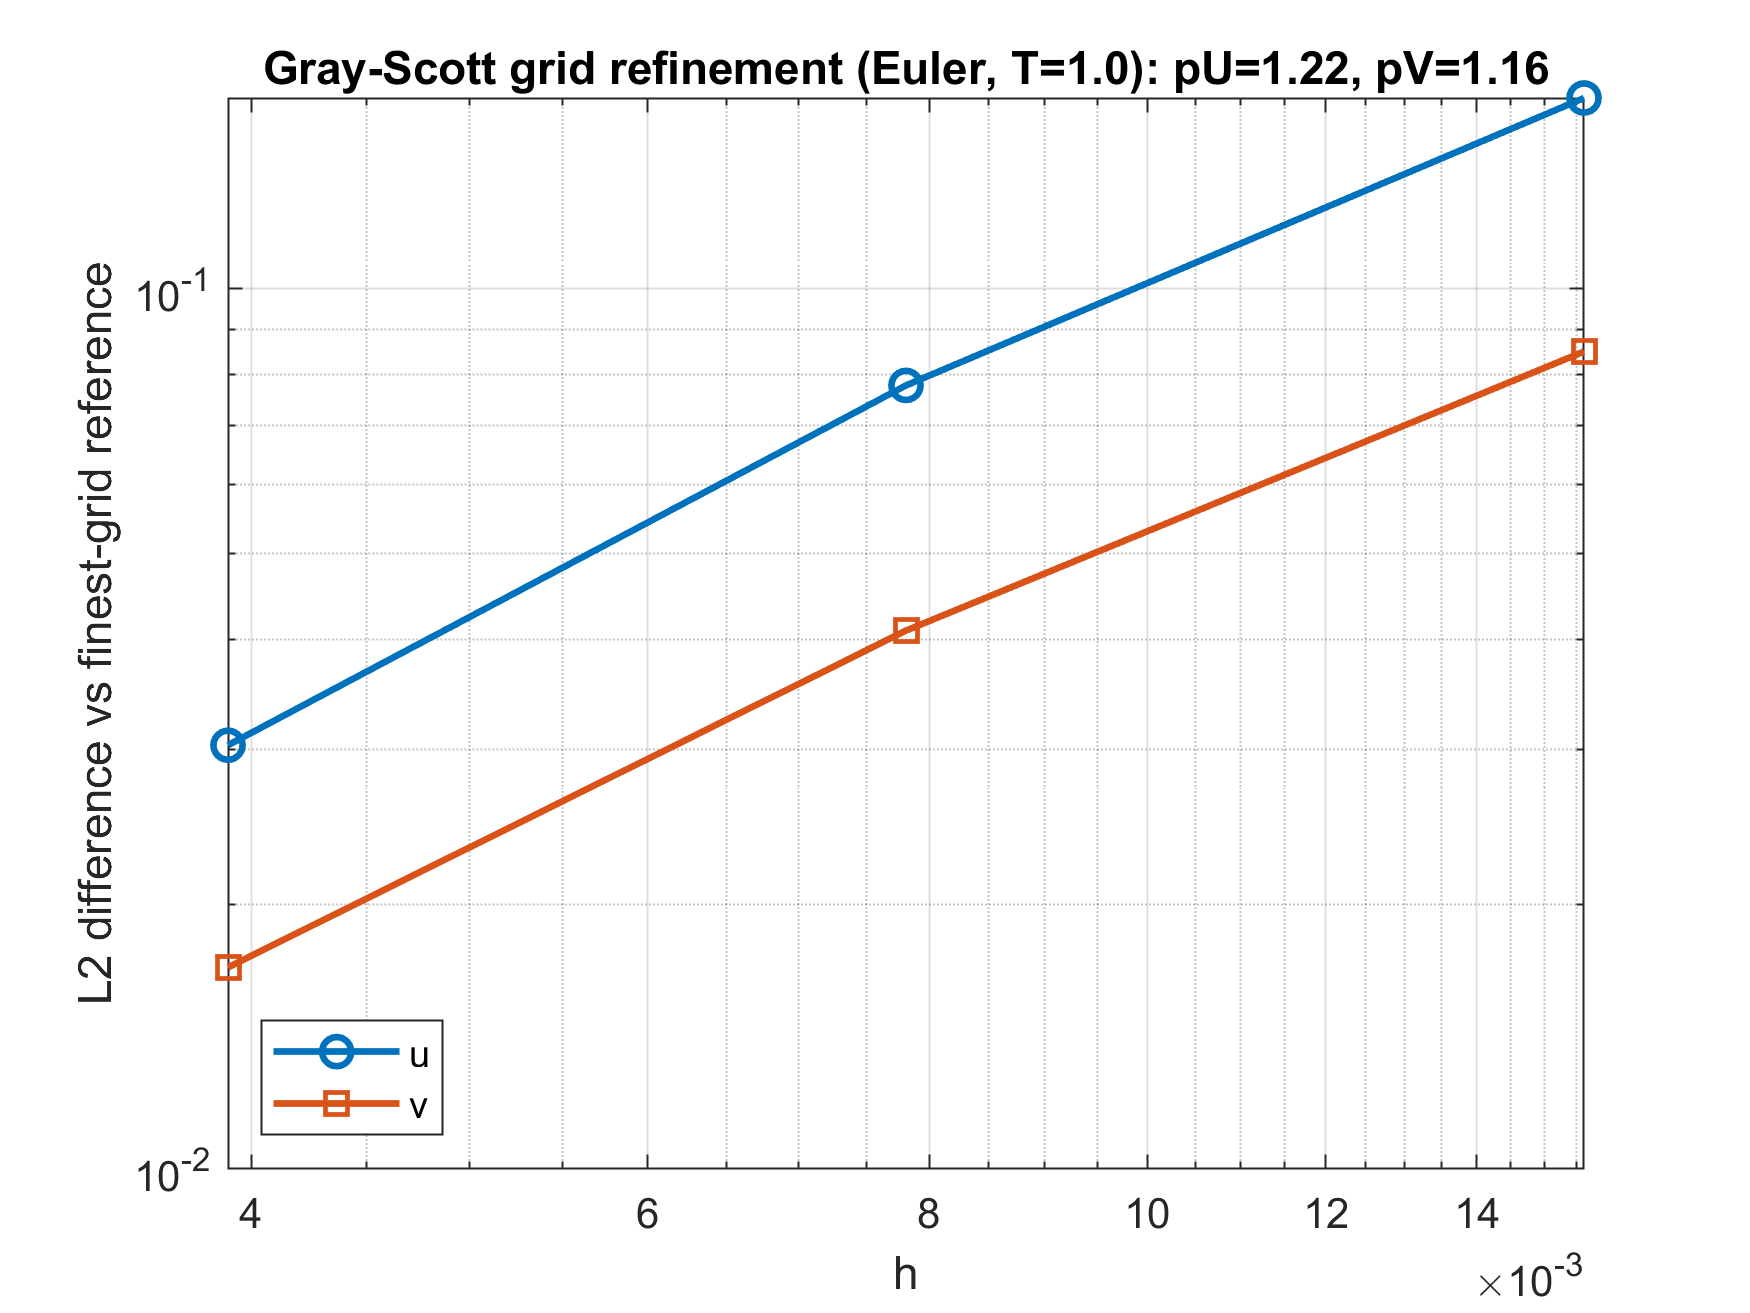
\includegraphics[width=0.82\textwidth]{figures/verification/grayscott_grid_refinement.png}
\caption{Final Gray--Scott grid-refinement study using the \(2048\times 2048\) solution as a numerical reference and a smooth grid-independent initial condition. The measured \(L^2\) differences in \(U\) and \(V\) decrease monotonically and yield observed rates \(p_U=p_V\approx 2.09\), consistent with second-order spatial behavior.}
\label{fig:grayscott_grid_refinement}
\end{figure}

\subsection{Test Case 8: Explicit Euler stability limit}
\label{sec:verification_testcase_explicit_stability_limit}

\paragraph{Aim.}
This test case verifies that the explicit Euler time integration used in the solver exhibits the correct conditional stability behavior for the diffusion part of the model. In contrast to the convergence tests, the purpose here is not to measure accuracy, but to check whether the implemented scheme obeys the theoretically known critical time-step limit. This is an important verification step because, for explicit methods, stability is a fundamental numerical property that must be reproduced correctly by the implementation.

\paragraph{Setup.}
The test is carried out in a controlled pure-diffusion subcase of the implemented Gray--Scott solver. To remove the reaction terms, the parameters are set to
\[
F = 0, \qquad k = 0,
\]
and the second species is initialized as
\[
v \equiv 0.
\]
As a result, the reaction part vanishes identically and the test isolates the explicit Euler discretization of the diffusion operator.

The computation is performed on a periodic square grid with
\[
N_x = N_y = 128.
\]
The diffusion coefficient of the first species is
\[
D_u = 2 \times 10^{-5},
\]
while \(D_v\) is irrelevant in this test because \(v\) remains zero throughout.

To excite the most restrictive mode for stability, the initial condition for \(u\) is chosen as a checkerboard perturbation around the constant mean state:
\[
u(x,y,0) = 1 + 0.1\,(-1)^{i+j}.
\]
This corresponds to the highest-frequency periodic mode of the discrete five-point Laplacian on an even grid. For this mode, the explicit Euler amplification factor is known analytically as
\[
g = 1 - \Delta t\,D_u\,\lambda_{\max},
\]
where
\[
\lambda_{\max} = \frac{4}{h_x^2} + \frac{4}{h_y^2}.
\]
Therefore, the critical time step is
\[
\Delta t_{\mathrm{crit}} = \frac{2}{D_u\,\lambda_{\max}}.
\]

For the documented run, this gives
\[
\Delta t_{\mathrm{crit}} = 0.762939.
\]
Three cases are then tested:
\[
\Delta t = 0.9\,\Delta t_{\mathrm{crit}}, \qquad
\Delta t = 1.0\,\Delta t_{\mathrm{crit}}, \qquad
\Delta t = 1.1\,\Delta t_{\mathrm{crit}}.
\]
Thus, the actual time-step values used are
\[
\Delta t \in \{0.68664551,\;0.76293945,\;0.83923340\}.
\]

Each case is advanced for
\[
n_{\text{steps}} = 20
\]
explicit Euler steps. At every step, the discrete \(L^2\) norm of the perturbation
\[
u - 1
\]
is measured. In addition to the observed one-step amplification factor, the complete measured norm history is compared against the theoretical history
\[
\|e^n\| = \|e^0\|\,|g|^n.
\]

\paragraph{How to run the test case.}
From the project \texttt{tests} folder, run:
\begin{verbatim}
r = test_explicit_stability_limit();
\end{verbatim}

The test prints the measured amplification factors and final norm ratios, and saves the generated figure in the local output folder of
\begin{verbatim}
tests/test_case_08_explicit_stability_limit/
\end{verbatim}

\paragraph{Expected result.}
For explicit Euler applied to diffusion, the expected behavior is classical:

\begin{itemize}
    \item if \(\Delta t < \Delta t_{\mathrm{crit}}\), the perturbation should decay;
    \item if \(\Delta t = \Delta t_{\mathrm{crit}}\), the perturbation norm should be preserved;
    \item if \(\Delta t > \Delta t_{\mathrm{crit}}\), the perturbation should grow, indicating instability.
\end{itemize}

For the chosen checkerboard mode, the theoretical one-step amplification factors are
\[
|g| = 0.8,\qquad 1.0,\qquad 1.2
\]
for the three tested cases. Therefore, the measured one-step amplification factors should agree with these values, and the full perturbation-norm history should follow the corresponding theoretical geometric behavior.

\paragraph{Obtained result.}
The test completed successfully, and the returned result was
\[
\texttt{pass} = 1.
\]

The MATLAB output reported:
\begin{verbatim}
case 1: dt = 0.68664551 = 0.90 dtCrit, g_theory = 0.800000,
        g_obs = 0.800000, final/initial = 0.011529,
        histRelErr = 3.247e-14

case 2: dt = 0.76293945 = 1.00 dtCrit, g_theory = 1.000000,
        g_obs = 1.000000, final/initial = 1.000000,
        histRelErr = 4.996e-15

case 3: dt = 0.83923340 = 1.10 dtCrit, g_theory = 1.200000,
        g_obs = 1.200000, final/initial = 38.337600,
        histRelErr = 9.415e-13
\end{verbatim}

The results are summarized in Table~\ref{tab:explicit_stability_limit}. In the subcritical case,
\[
\Delta t = 0.9\,\Delta t_{\mathrm{crit}},
\]
the perturbation decayed strongly, with final-to-initial ratio
\[
0.011529.
\]
At the critical value,
\[
\Delta t = \Delta t_{\mathrm{crit}},
\]
the perturbation norm was preserved exactly:
\[
\frac{\|e^{20}\|}{\|e^0\|} = 1.
\]
In the supercritical case,
\[
\Delta t = 1.1\,\Delta t_{\mathrm{crit}},
\]
the perturbation grew rapidly, with final-to-initial ratio
\[
38.337600.
\]

Most importantly, the measured one-step amplification factors matched the theoretical values exactly in all three cases:
\[
g_{\mathrm{obs}} = g_{\mathrm{theory}} = \{0.8,\;1.0,\;1.2\}.
\]
Moreover, the maximum relative error between the complete measured norm history and the theoretical geometric history remained extremely small, with worst case
\[
9.415 \times 10^{-13}.
\]

\begin{table}[htbp]
\centering
\caption{Explicit Euler stability-limit test results for the diffusion subcase on the \(128\times128\) periodic grid.}
\label{tab:explicit_stability_limit}
\begin{tabular}{|c|c|c|c|c|}
\hline
Case & \(\Delta t / \Delta t_{\mathrm{crit}}\) & \(g_{\mathrm{theory}}\) & \(g_{\mathrm{obs}}\) & final/initial \\
\hline
stable     & 0.9 & 0.8 & 0.8 & 0.011529 \\
critical   & 1.0 & 1.0 & 1.0 & 1.000000 \\
unstable   & 1.1 & 1.2 & 1.2 & 38.337600 \\
\hline
\end{tabular}
\end{table}

Figure~\ref{fig:explicit_stability_limit} shows the normalized perturbation \(L^2\) norm as a function of Euler step. The subcritical case decays monotonically, the critical case remains constant, and the supercritical case grows exponentially. The figure therefore reproduces exactly the three theoretical stability regimes expected for the explicit Euler discretization of diffusion.

Hence, this test confirms that the implementation reproduces the correct stability boundary of the explicit Euler method. It verifies not only the qualitative behavior below, at, and above the critical time step, but also the quantitative amplification factors predicted by theory.

\begin{figure}[htbp]
\centering
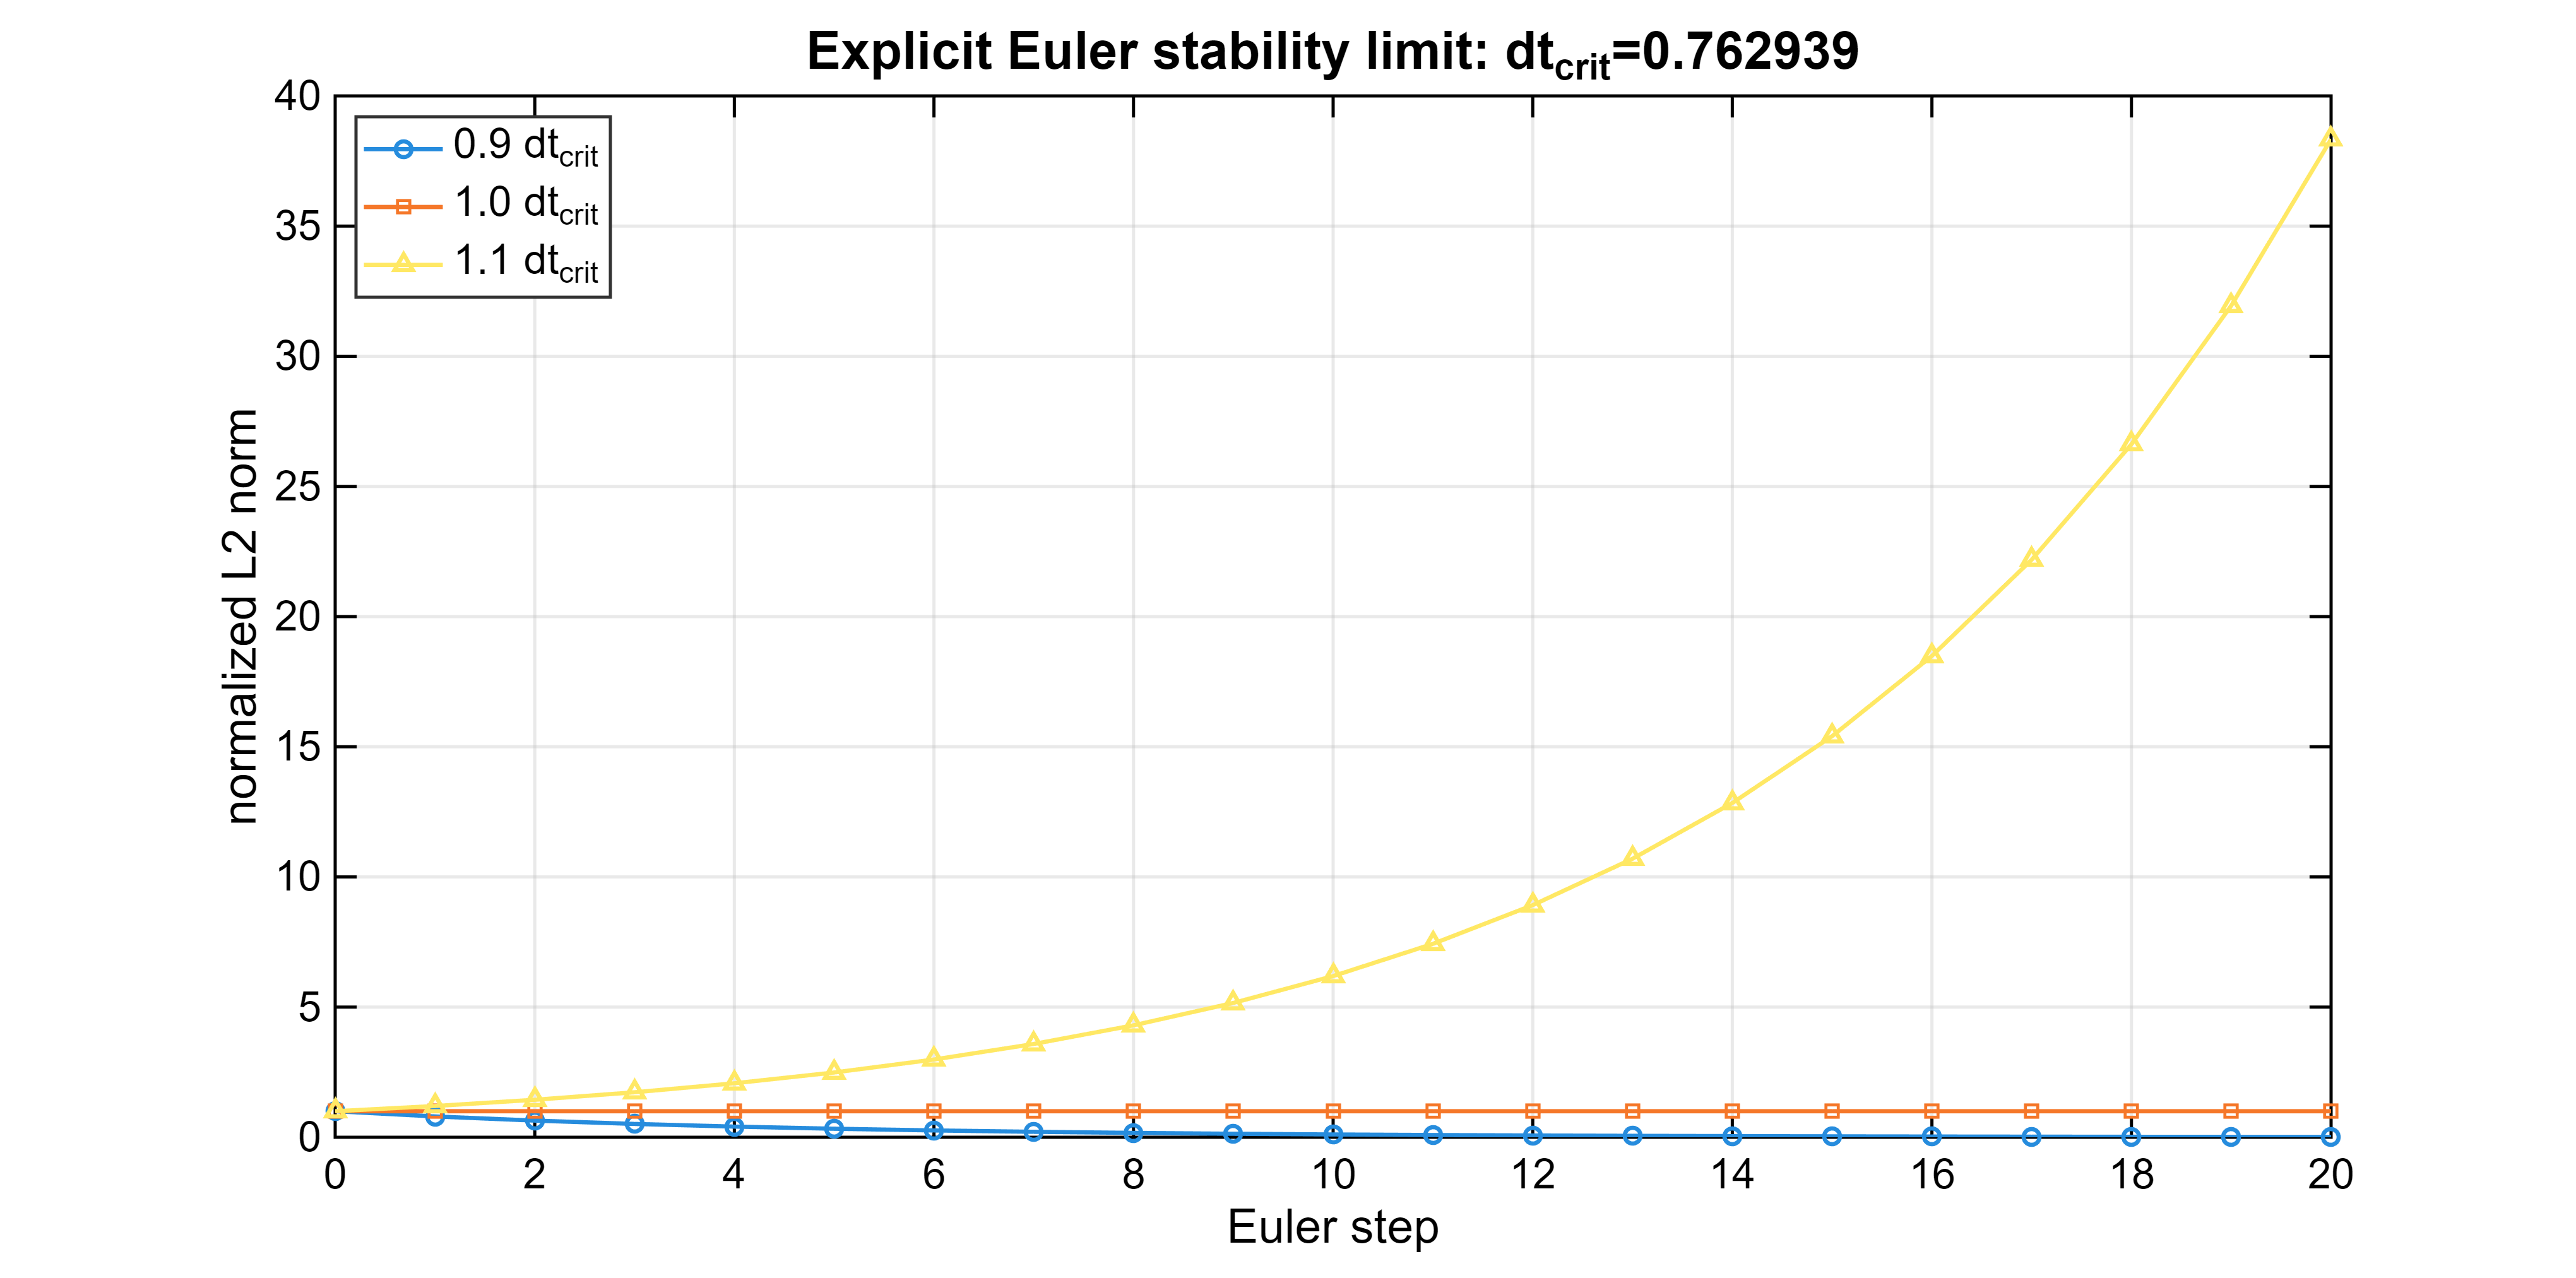
\includegraphics[width=0.82\textwidth]{figures/verification/explicit_stability_limit.png}
\caption{Explicit Euler stability-limit test for the diffusion subcase on the \(128\times128\) periodic grid. Below the critical time step the perturbation decays, at the critical value it is preserved, and above the critical value it grows, in exact agreement with the theoretical amplification factors.}
\label{fig:explicit_stability_limit}
\end{figure}

\section{Supplementary verification checks}
\label{sec:verification_supplementary}

In addition to the detailed test cases above, several smaller checks were carried out to support the overall verification strategy. These tests are useful because they isolate specific mathematical or implementation properties, even if they do not require a full standalone discussion.

\subsection{Constant-field Laplacian null test}
\label{sec:verification_constant_field}

As an additional structural check, the discrete Laplacian was applied to a constant field. For a constant function, the continuous Laplacian is identically zero, and the same property is expected from the discrete operator. Therefore, this test serves as a simple but useful sanity check of the assembled diffusion operator.

The test was executed with:
\begin{verbatim}
r = test_laplacian_constant();
\end{verbatim}

For the documented run, the returned result was
\[
\texttt{pass} = 1,
\]
with
\[
\|L\mathbf{1}\|_{\infty} = 0.000\times 10^{0},
\qquad
\|L\mathbf{1}\|_{2} = 0.000\times 10^{0}.
\]
Thus, the discrete Laplacian annihilates a constant field exactly in this case. This confirms that the operator satisfies an important basic consistency property and provides additional evidence that the diffusion discretization is assembled correctly.

\subsection{Symmetry check of the discrete Laplacian matrix}
\label{sec:verification_laplacian_symmetry}

A further structural verification step checks the symmetry of the assembled discrete Laplacian matrix. For the periodic finite-difference diffusion operator used in this project, the Laplacian matrix is expected to be symmetric under the tested setup. This property is important because it supports the correctness of the stencil-to-matrix assembly and helps detect indexing or coefficient-placement errors.

The test was executed with:
\begin{verbatim}
r = test_laplacian_symmetry();
\end{verbatim}

For the documented run, the returned result was
\[
\texttt{pass} = 1,
\]
and the reported symmetry defect was
\[
\|L - L^{T}\|_{\infty} = 0.000\times 10^{0}.
\]
Therefore, the assembled Laplacian matrix is exactly symmetric in this case. This result is fully consistent with the expected structure of the periodic diffusion operator and provides additional evidence that the matrix assembly is implemented correctly.

\subsection{End-to-end MMS consistency check}
\label{sec:verification_mms_endtoend}

As a supplementary verification step, the full solver was tested with a manufactured-solution setup. In contrast to the operator-only MMS test of Test Case~1, this check verifies the complete time-dependent workflow, including reaction, diffusion, source-term handling, and explicit Euler time stepping. It is therefore useful as supporting end-to-end verification evidence for the implemented numerical model.

The test was executed with:
\begin{verbatim}
r = test_mms_endtoend();
\end{verbatim}

For the documented run, the solver used a grid
\[
N_x=N_y=128,
\]
a time step
\[
\Delta t = 0.01,
\]
and a final time
\[
T = 1.
\]
The returned result was
\[
\texttt{pass} = 1,
\]
and the reported final \(L^2\) errors were
\[
\mathrm{err}_U^{L^2} = 1.179\times 10^{-4},
\qquad
\mathrm{err}_V^{L^2} = 5.974\times 10^{-4}.
\]

These errors are small for the chosen grid and time-step size. They are consistent with a correctly implemented manufactured-solution workflow. The generated error figure is stored in the local output folder of \texttt{tests/supplementary\_checks/}. Figure~\ref{fig:mms_endtoend_errV} shows the spatial error field for \(v\) at the final time. The smooth, structured pattern is typical of discretization error and does not indicate instability or implementation failure.

\begin{figure}[htbp]
\centering
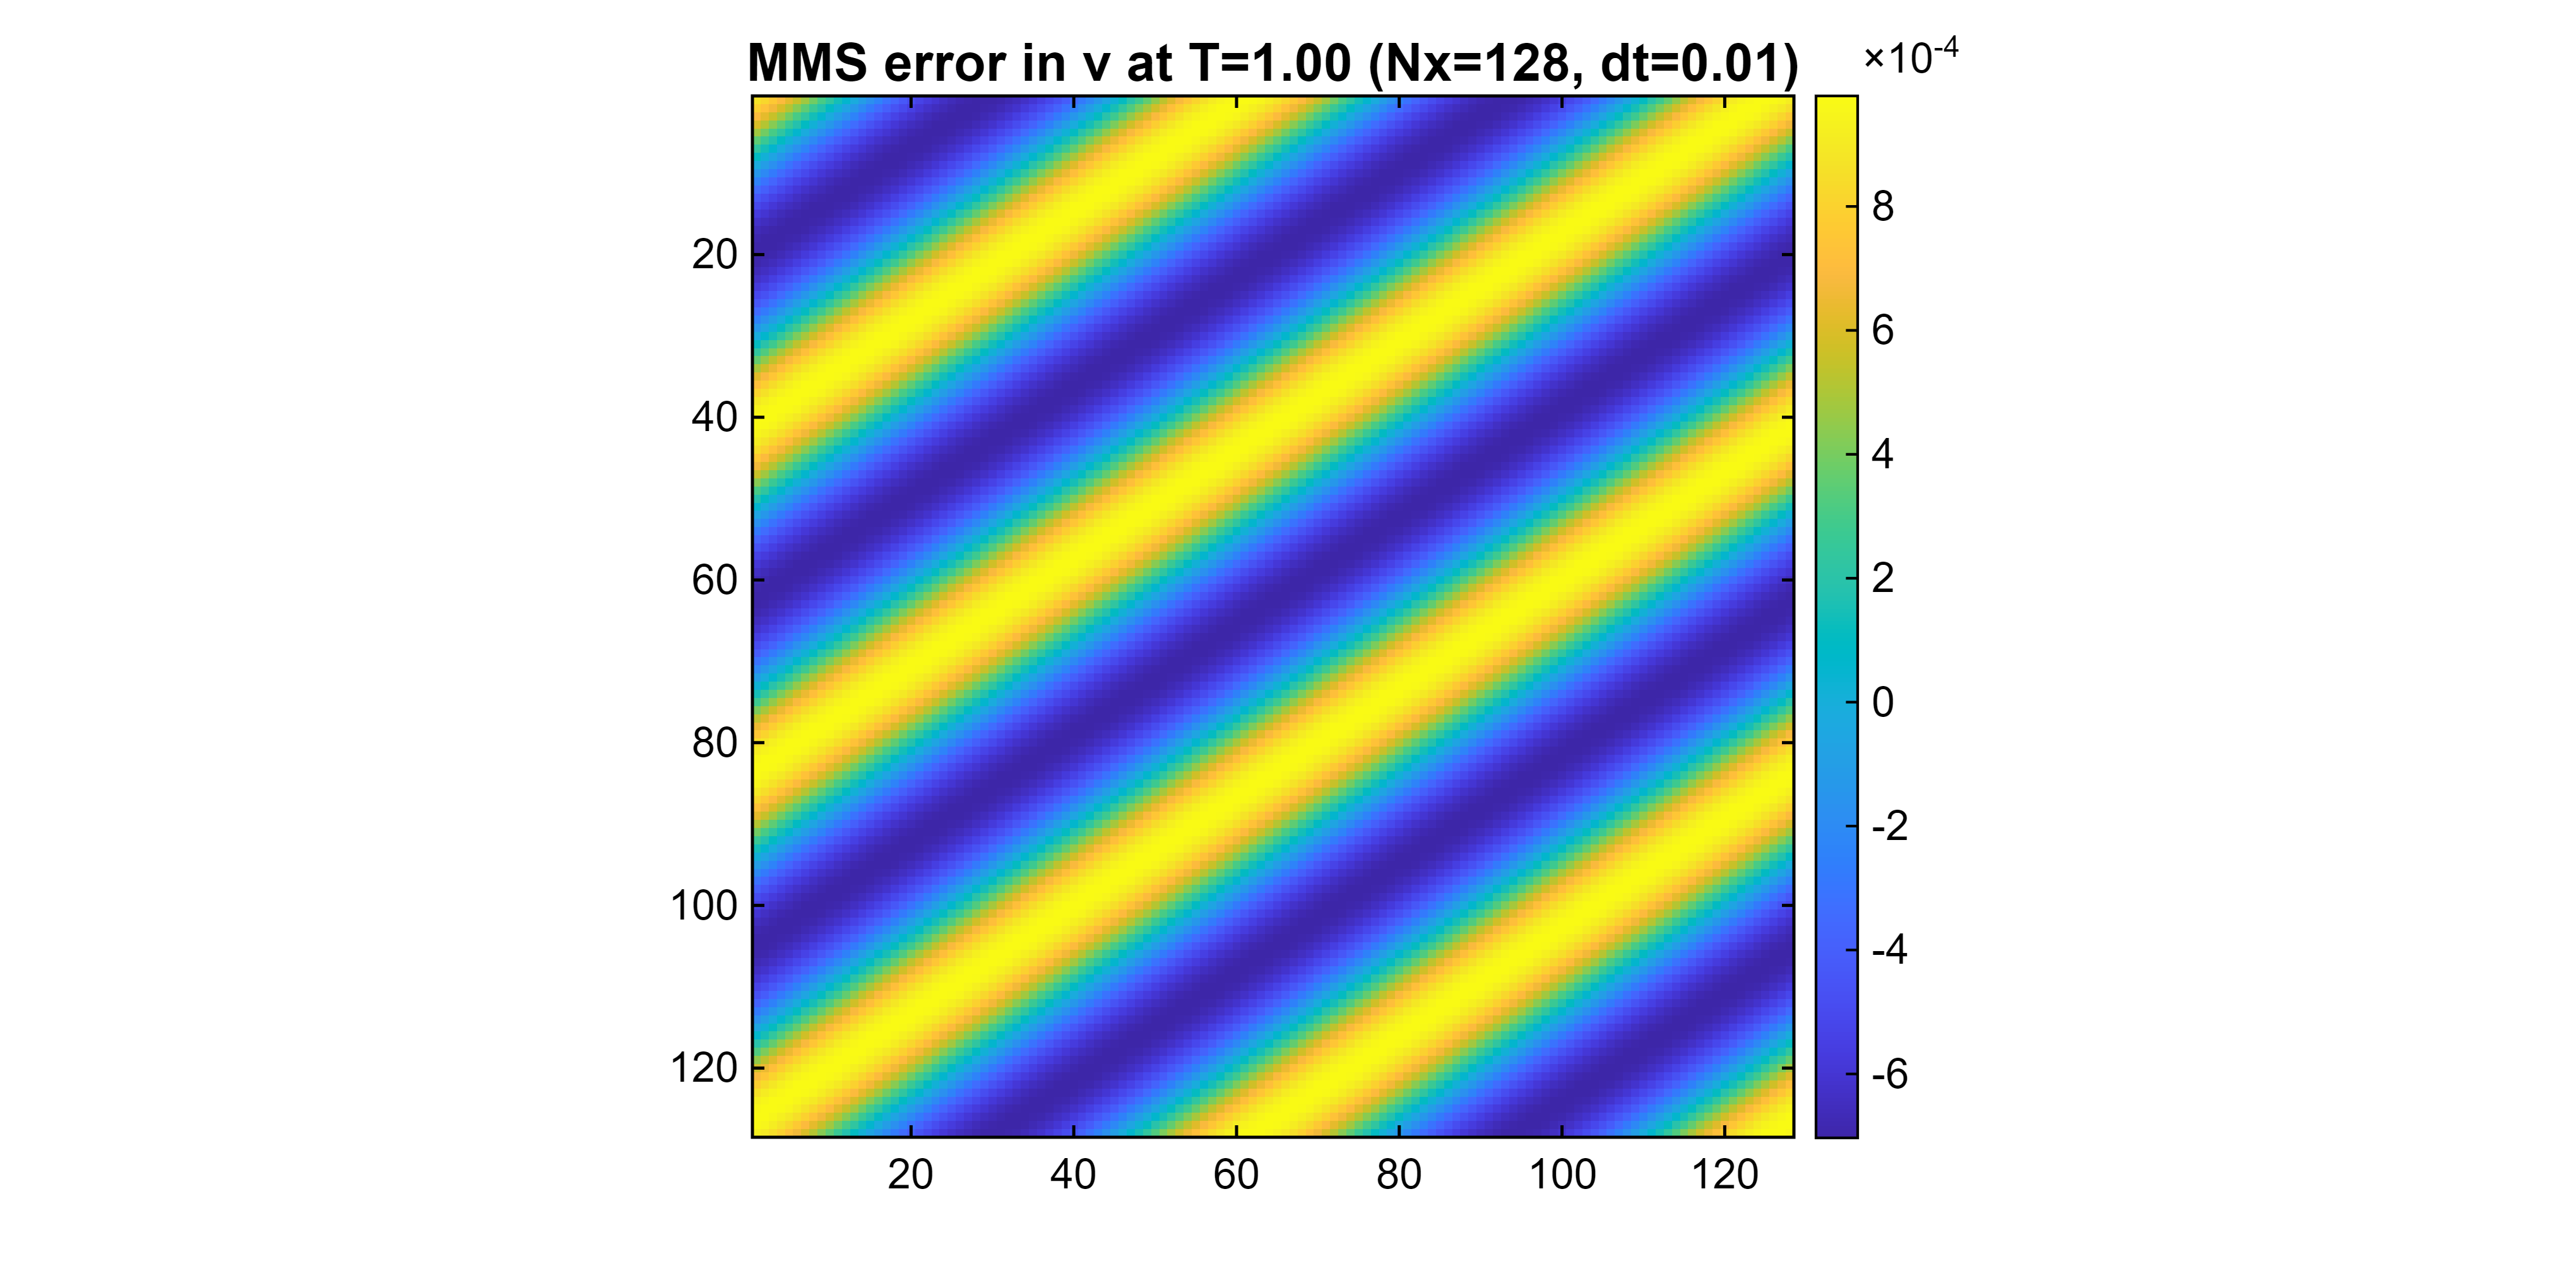
\includegraphics[width=0.72\textwidth]{figures/verification/mms_endtoend_errV.png}
\caption{Spatial error field of the manufactured-solution end-to-end test for \(v\) at \(T=1\), with \(N_x=N_y=128\) and \(\Delta t=0.01\).}
\label{fig:mms_endtoend_errV}
\end{figure}

Overall, this supplementary test provides additional evidence that the complete solver reproduces the manufactured solution with small final errors when the corresponding source terms are included.

\subsection{Time-step halving smoke test}
\label{sec:verification_timestep_halving_smoke}

As a quick supplementary consistency check, a simpler time-step halving test was also performed. In contrast to the full temporal convergence study of Test Case~2, this test is not intended as a rigorous order-verification procedure. Instead, it serves as a compact sanity check showing that the numerical solution changes in the expected direction when the time step is refined.

The test was executed with:
\begin{verbatim}
r = test_timestep_halving_smoke();
\end{verbatim}

For the documented run, the solver used a grid
\[
N_x=N_y=128,
\]
a final time
\[
T=50,
\]
and the baseline time step
\[
\Delta t = 0.2.
\]
The returned result was
\[
\texttt{pass} = 1,
\]
and the reported differences between successive refinements were
\[
\mathrm{rms}_{12} = 3.706\times 10^{-5}, \qquad
\mathrm{rms}_{24} = 1.851\times 10^{-5},
\]
\[
\mathrm{inf}_{12} = 5.798\times 10^{-4}, \qquad
\mathrm{inf}_{24} = 2.891\times 10^{-4}.
\]

The finer-step differences are smaller than the coarser-step differences in both norms:
\[
\mathrm{rms}_{24} < \mathrm{rms}_{12},
\qquad
\mathrm{inf}_{24} < \mathrm{inf}_{12}.
\]
Moreover, the reduction is approximately by a factor of two, which is consistent with the expected first-order behavior of the explicit Euler method under time-step halving.


\section{Validation-oriented pattern sanity check}
\label{sec:verification_pattern_sanity}

In addition to the formal verification tests presented earlier in this chapter, a long-time Gray--Scott pattern study was carried out as a \emph{validation-oriented sanity check}. The role of this section is intentionally different from that of the preceding test cases. The earlier tests were designed to verify numerical correctness in a strict sense, for example through manufactured solutions, convergence measurements, operator equivalence, boundary-condition enforcement, and consistency checks between different execution paths. By contrast, the present study asks whether the implemented solver also reproduces the kind of plausible and morphologically distinct pattern classes that are commonly associated with the Gray--Scott model in the literature.

The Gray--Scott system is well known for producing a rich variety of self-organized structures depending on the feed and kill parameters. Pearson's classical study established the basic pattern-forming context of the model, while later classification work organized a broader range of visually distinct regimes using labels such as \texttt{alpha}, \texttt{epsilon}, \texttt{kappa}, and \texttt{theta} \cite{pearson1993,munafo_gray_scott_classes}. A modern tutorial-style analysis of the Gray--Scott model and its pattern behavior is also given in \cite{gandy2022}. The present test is therefore not intended to replace the formal verification evidence, but rather to complement it by showing that the final implementation produces stable and qualitatively reasonable long-time dynamics for standard Pearson-type parameter choices.

\subsection{Test Case 9: Pearson-type pattern sanity check}
\label{sec:verification_testcase_pearson}

\paragraph{Aim.}
This test case checks whether the implemented solver reproduces visually reasonable Gray--Scott patterns for several Pearson-type parameter sets over a long simulation horizon. The aim is not to verify a convergence order or to compare against an exact analytical solution, but to confirm that the final implementation is capable of producing the expected diversity of Gray--Scott morphologies under standard long-time conditions. More specifically, the test examines whether different parameter choices lead to clearly different and stable pattern classes rather than to numerical noise, spurious artifacts, or an incorrect collapse to a trivial state.

\paragraph{Setup.}
The test uses the Pearson preset on the periodic square domain
\[
\Omega = [0,1)\times[0,1)
\]
with a uniform grid
\[
N_x = N_y = 256.
\]
The time step is
\[
\Delta t = 1,
\]
and each case is simulated for
\[
N_t = 200000
\]
time steps, corresponding to the final time
\[
T = 200000.
\]
The diffusion coefficients are
\[
D_u = 2\times 10^{-5}, \qquad D_v = 1\times 10^{-5},
\]
and periodic boundary conditions are imposed on all sides.

Four Pearson-type parameter sets are tested:
\[
\texttt{alpha}: \quad F=0.0075294,\qquad k=0.04564,
\]
\[
\texttt{kappa}: \quad F=0.034487,\qquad k=0.060378,
\]
\[
\texttt{epsilon}: \quad F=0.019707,\qquad k=0.055379,
\]
\[
\texttt{theta}: \quad F=0.040117,\qquad k=0.060515.
\]

For each case, snapshots of the \(U\)- and \(V\)-fields are saved at
\[
t = 50000,\;100000,\;150000,\;200000.
\]
In the present report, the \(U\)-field snapshots at
\[
t = 100000
\]
are used for comparison, because at this time the morphology of each case is already well developed while still being easy to interpret visually.

\paragraph{How to run the test case.}
From the project \texttt{tests} folder, run:
\begin{verbatim}
r = test_pattern_sanity_pearson();
\end{verbatim}

The test saves the generated images in the local output folder of
\begin{verbatim}
tests/test_case_09_pearson_pattern_sanity/
\end{verbatim}
and, for the documented run, completed all four cases successfully. The MATLAB output reported that snapshots were saved for all four parameter sets at
\[
t=50000,\;100000,\;150000,\;200000,
\]
and that the full run finished for the cases
\[
\texttt{alpha},\;\texttt{kappa},\;\texttt{epsilon},\;\texttt{theta}.
\]

\paragraph{Expected result.}
Since this is a validation-oriented sanity check, the expected result is qualitative rather than pointwise exact. One expects the simulation to produce stable, visually structured Gray--Scott patterns whose morphology depends strongly on the chosen \((F,k)\) pair. In particular, different Pearson-type labels should not all lead to nearly identical images. Instead, some cases should favor spot-dominated structures, while others should exhibit more elongated stripe-like or labyrinthine organizations \cite{pearson1993,munafo_gray_scott_classes}. The important criterion is therefore not exact agreement with a single published image, but rather the emergence of distinct and plausible pattern classes under long-time integration. As a supporting modern reference, \cite{gandy2022} also discusses the sensitivity of Gray--Scott pattern formation to parameter choice.

\paragraph{Obtained result.}
The test completed successfully, and the returned result was
\[
\texttt{pass} = 1.
\]
Each of the four parameter sets was simulated over the full
\[
200000
\]
time steps, and all requested snapshots were saved.
The representative \(U\)-field snapshots at \(t=100000\), shown in Figs.~\ref{fig:pearson_alpha_snapshot}--\ref{fig:pearson_theta_snapshot}, demonstrate that the implemented solver generates clearly different and visually plausible pattern morphologies for the four tested parameter sets.

The \texttt{alpha} case in Fig.~\ref{fig:pearson_alpha_snapshot} is dominated by separated spot-like structures embedded in a mostly high-\(U\) background. The spots are irregularly distributed, but they remain localized and well formed. The image does not suggest numerical breakup, grid-aligned artifacts, or unstable oscillatory contamination. Instead, it shows a coherent spot-dominated regime consistent with the expected Gray--Scott behavior for this type of parameter choice.

The \texttt{epsilon} case in Fig.~\ref{fig:pearson_epsilon_snapshot} also belongs to a spot-dominated family, but the pattern is markedly denser and more crowded than in the \texttt{alpha} case. Small spot-like depressions in the \(U\)-field are distributed much more uniformly across the domain, producing a texture that is finer and more tightly packed. This visual difference is important because it shows that the solver is not merely reproducing one generic spot pattern for all parameter values; rather, it responds sensitively to the change in \((F,k)\) and produces a distinctly different morphological regime.

By contrast, the \texttt{kappa} case in Fig.~\ref{fig:pearson_kappa_snapshot} is no longer spot-dominated. Instead, the solution organizes into broad, elongated, stripe-like structures with a labyrinthine appearance. The stripes are smooth and continuous over long distances, and they form an interconnected network rather than isolated islands. This is a qualitatively different regime from the previous two cases and is visually consistent with the classic Gray--Scott transition from spot patterns to stripe or maze-like patterns under different parameter settings.

The \texttt{theta} case in Fig.~\ref{fig:pearson_theta_snapshot} is also labyrinth-like, but it is not identical to \texttt{kappa}. The stripe network is more intricate and locally more curved, and the overall topology appears somewhat more tangled and fine-scaled. Thus, even within the stripe-dominated family, the implementation still distinguishes between parameter sets and produces visibly different structure. This strengthens the interpretation that the solver is capturing meaningful qualitative pattern dependence rather than generating a single repeated texture.

Taken together, these four cases show two important features. First, the runs remain numerically stable and visually clean over a very long integration horizon. Second, the parameter changes lead to clear morphological differentiation between spot-dominated and labyrinth-dominated regimes, with further variation inside each family. This is exactly the kind of application-level behavior expected from a plausible Gray--Scott implementation \cite{pearson1993,munafo_gray_scott_classes}.

At the same time, the interpretation of this test should remain careful. Because no exact reference field is available, the present result does not prove correctness in the same way as the manufactured-solution or convergence-based tests. Its role is supportive: it shows that the implemented model behaves plausibly, produces stable long-time structures, and reproduces the qualitative diversity associated with Pearson-type Gray--Scott dynamics.

\begin{figure}[htbp]
\centering
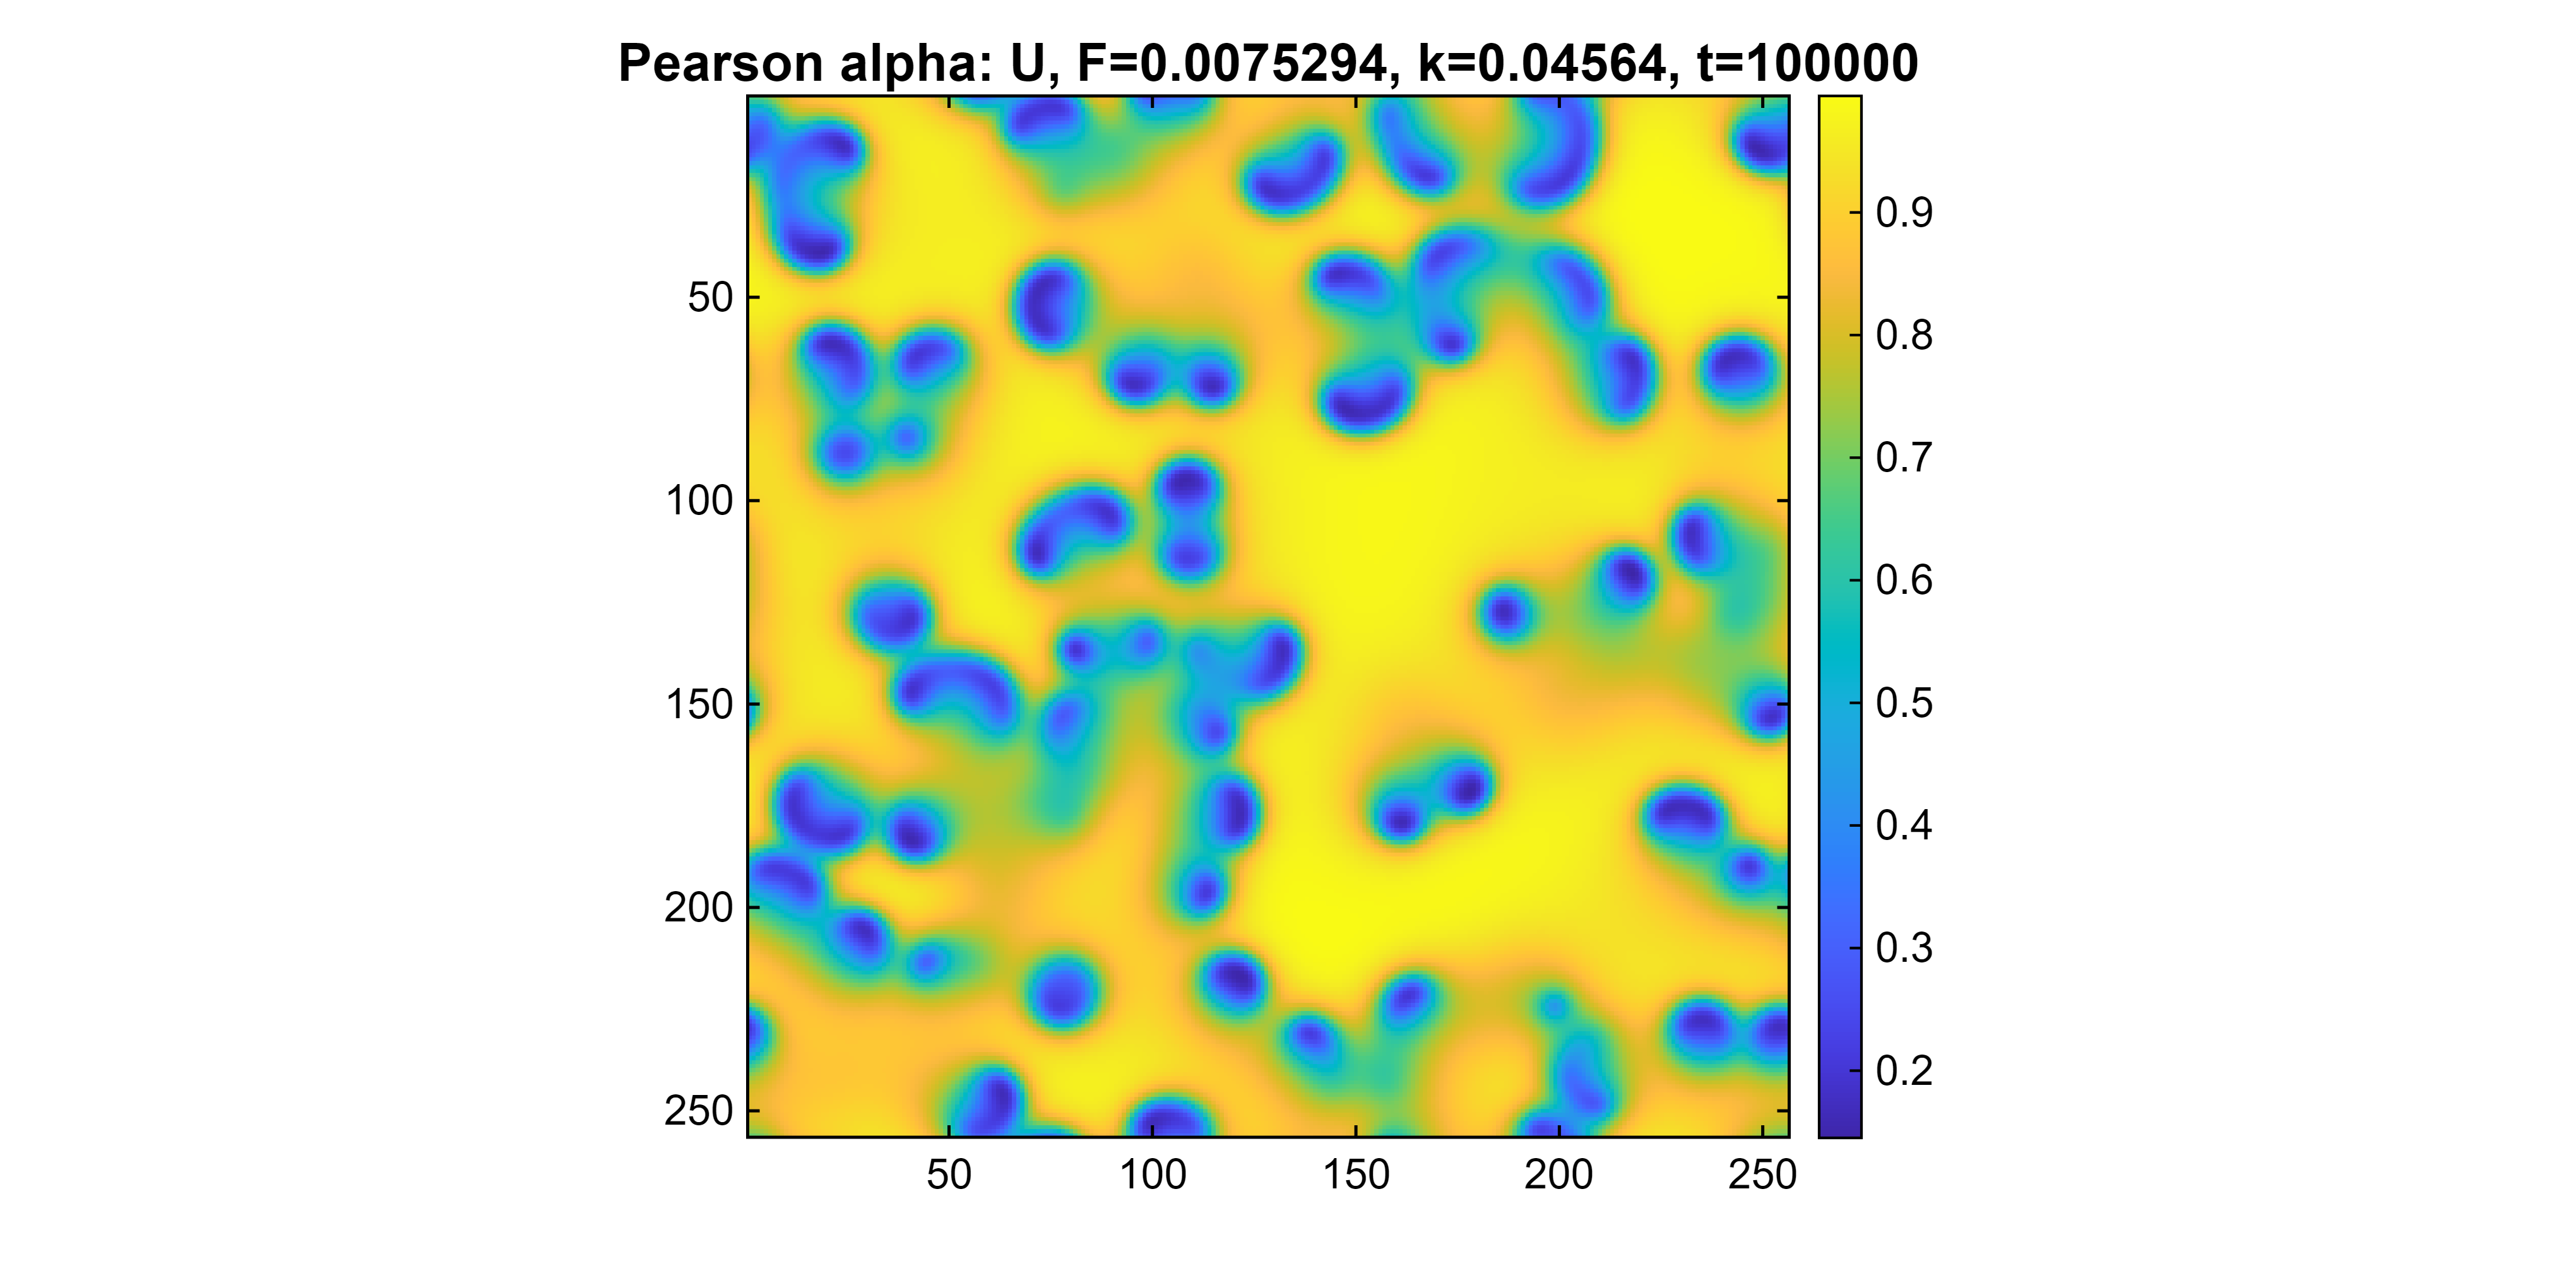
\includegraphics[width=0.95\textwidth]{figures/verification/pattern_sanity/alpha_t100000_U.png}
\caption{Pearson \texttt{alpha} case: representative \(U\)-field snapshot at \(t=100000\). The morphology is dominated by separated spot-like structures in a mostly high-\(U\) background.}
\label{fig:pearson_alpha_snapshot}
\end{figure}

\begin{figure}[htbp]
\centering
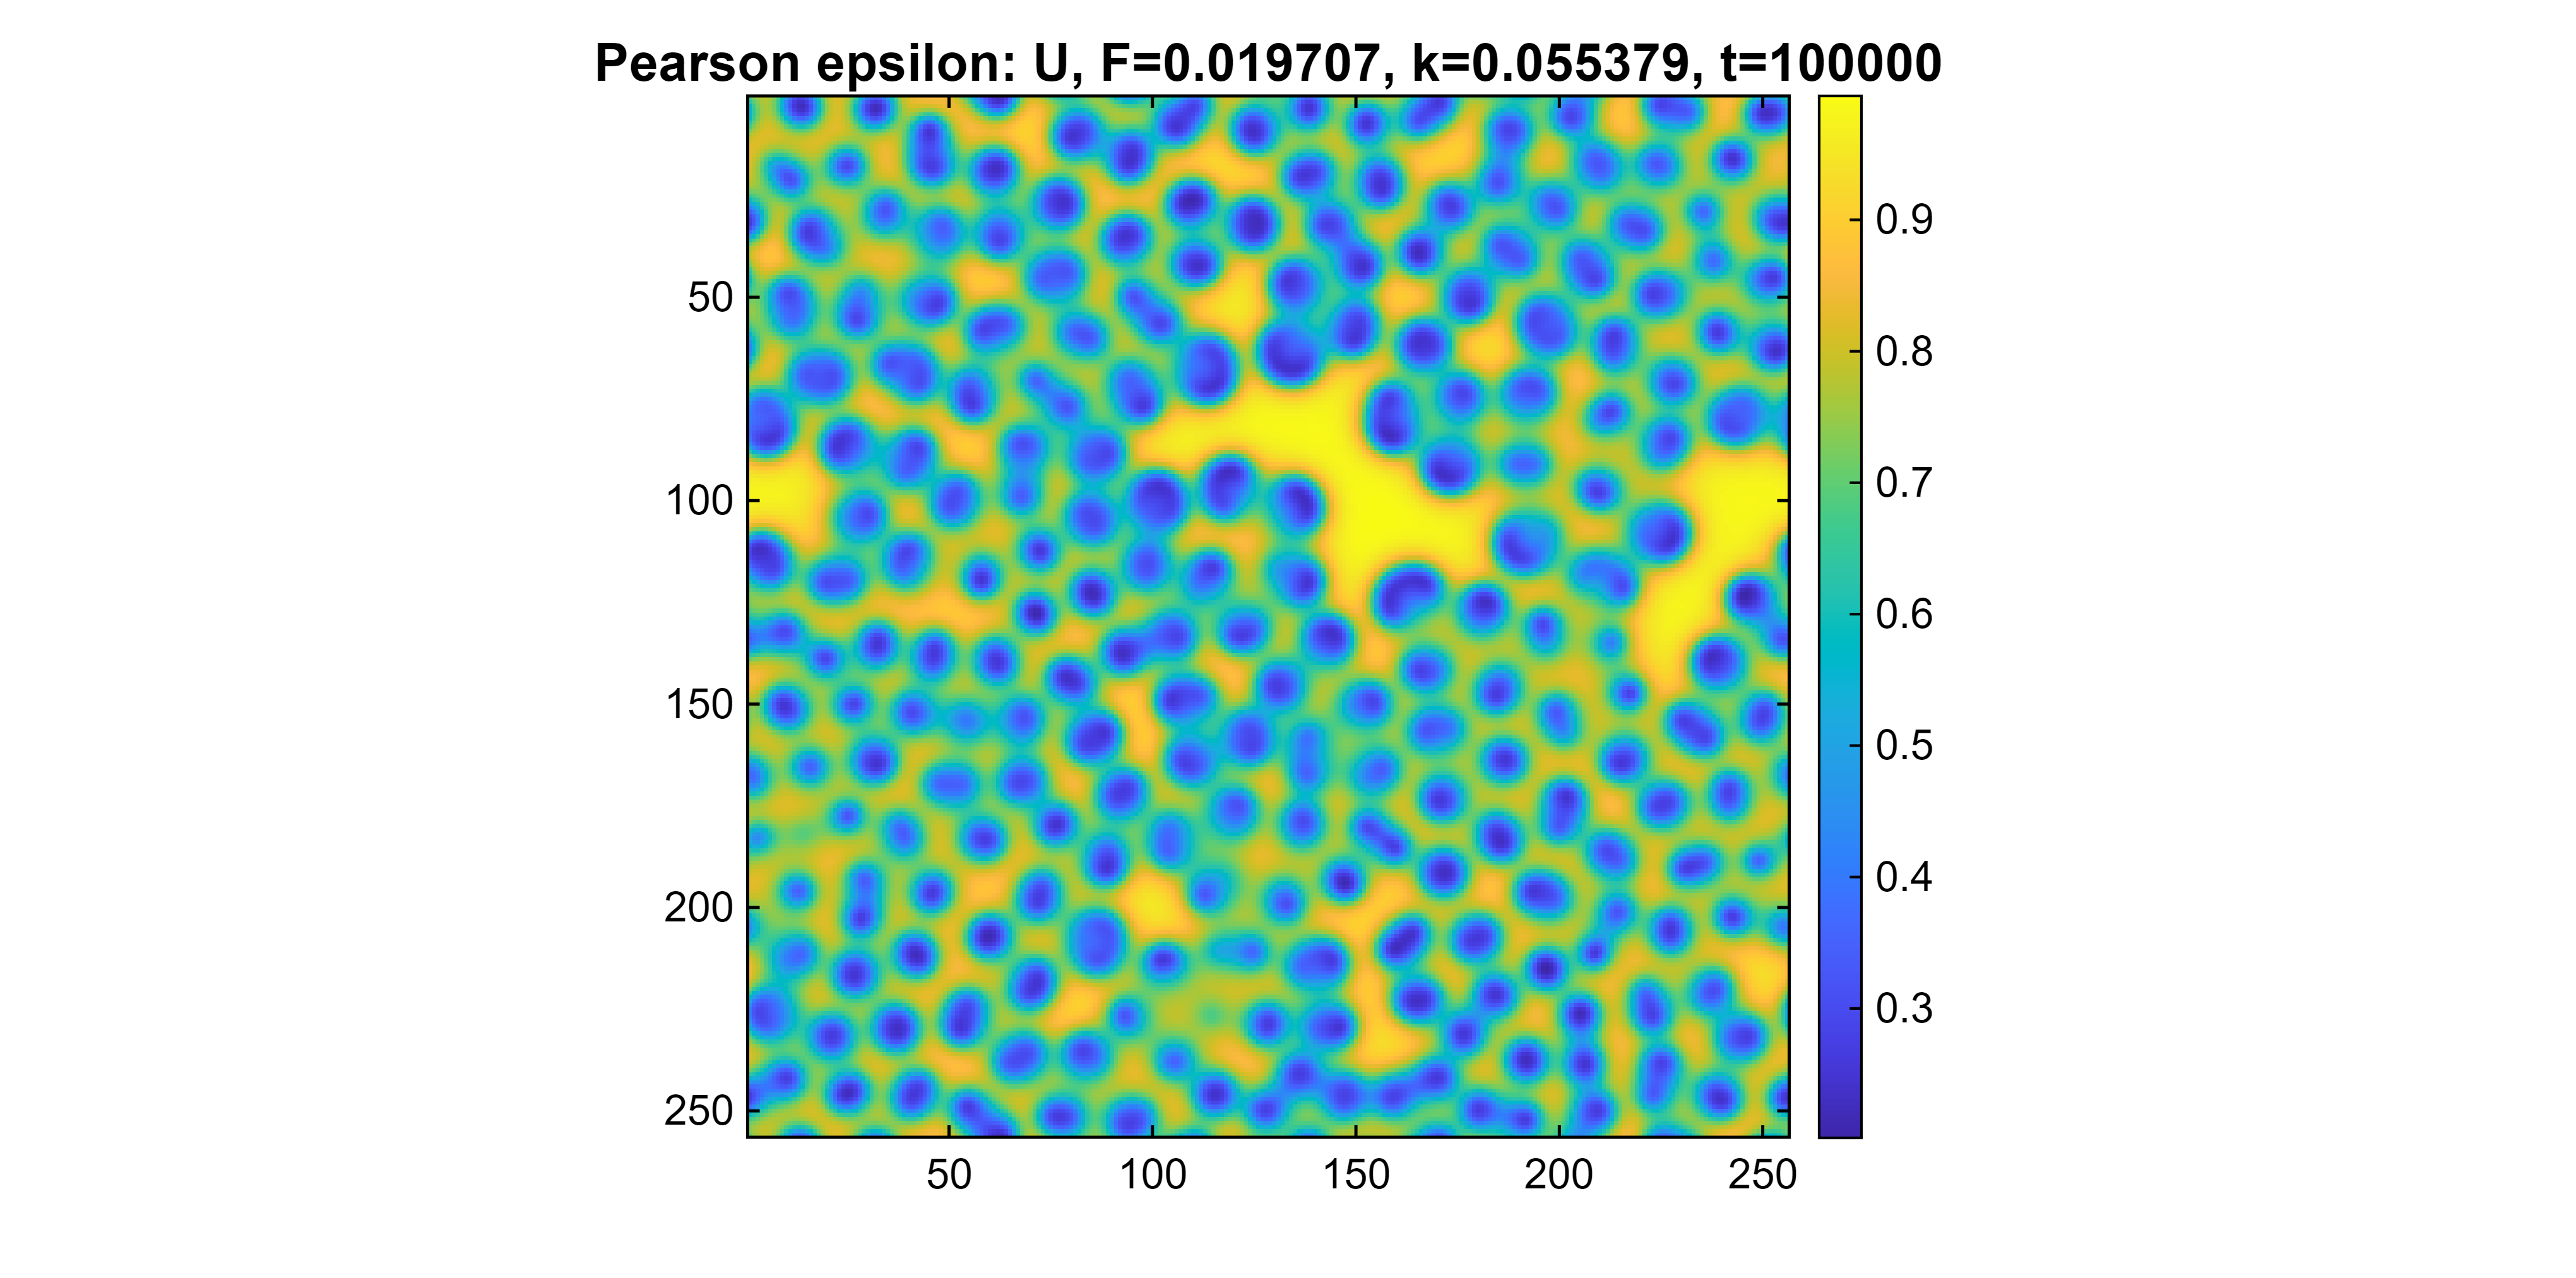
\includegraphics[width=0.95\textwidth]{figures/verification/pattern_sanity/epsilon_t100000_U.png}
\caption{Pearson \texttt{epsilon} case: representative \(U\)-field snapshot at \(t=100000\). Compared with \texttt{alpha}, the pattern is denser and more uniformly populated by small spot-like structures.}
\label{fig:pearson_epsilon_snapshot}
\end{figure}

\begin{figure}[htbp]
\centering
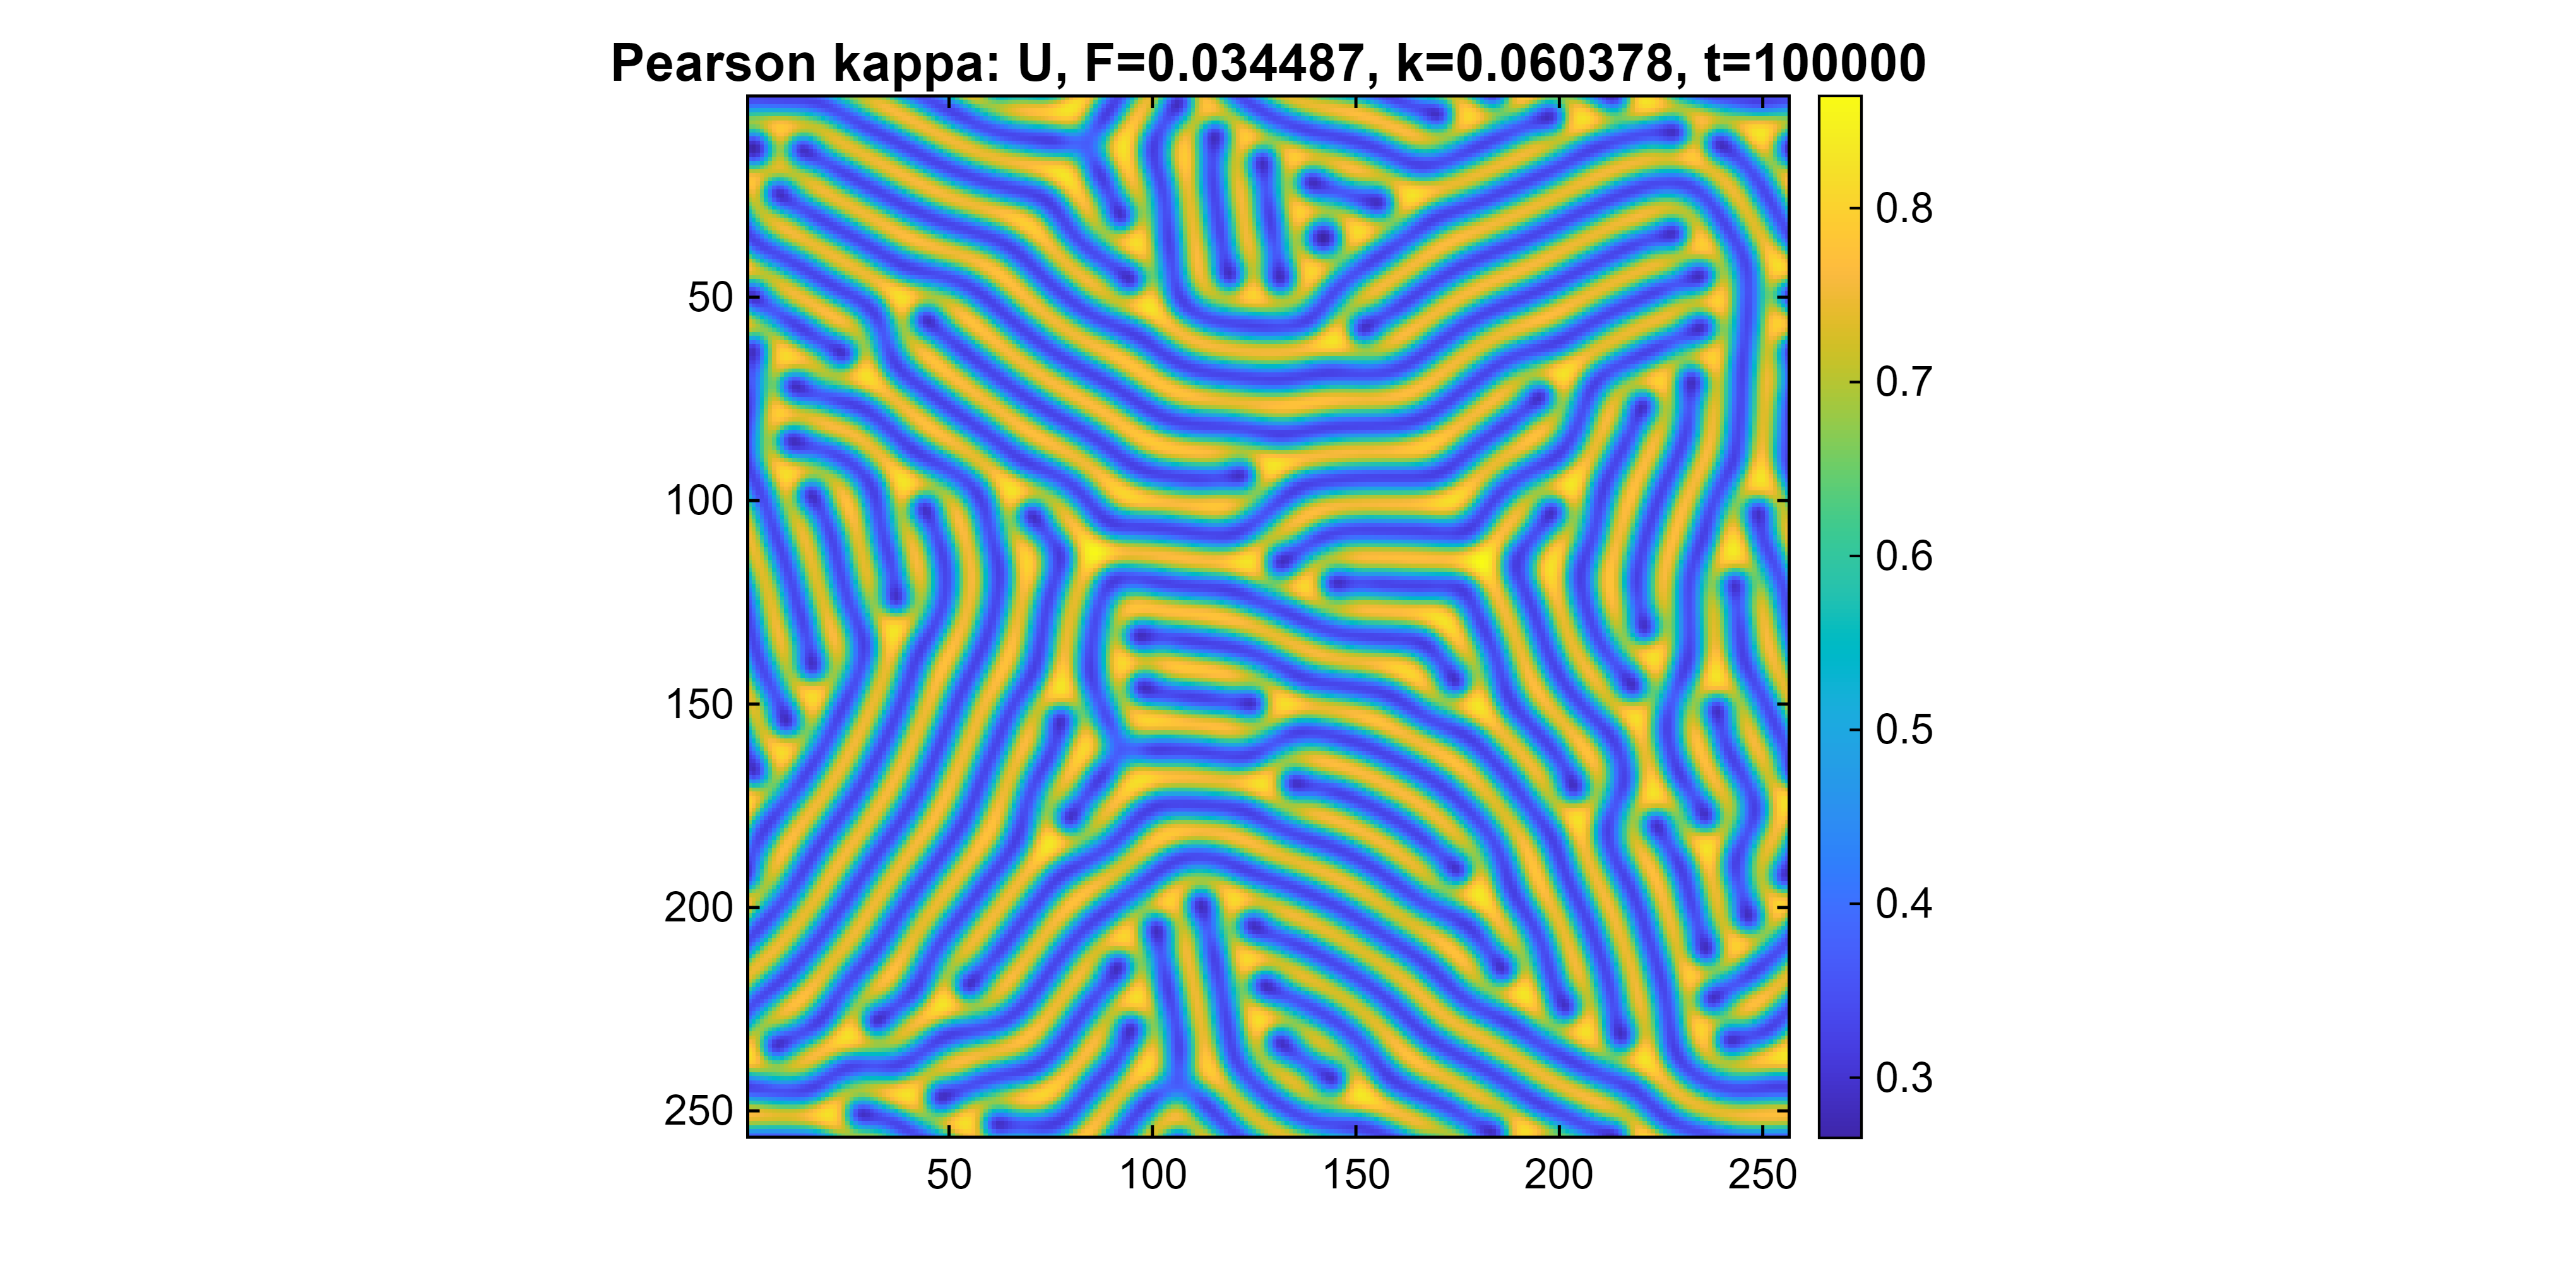
\includegraphics[width=0.95\textwidth]{figures/verification/pattern_sanity/kappa_t100000_U.png}
\caption{Pearson \texttt{kappa} case: representative \(U\)-field snapshot at \(t=100000\). The pattern exhibits a broad labyrinth-like stripe morphology rather than isolated spots.}
\label{fig:pearson_kappa_snapshot}
\end{figure}

\begin{figure}[htbp]
\centering
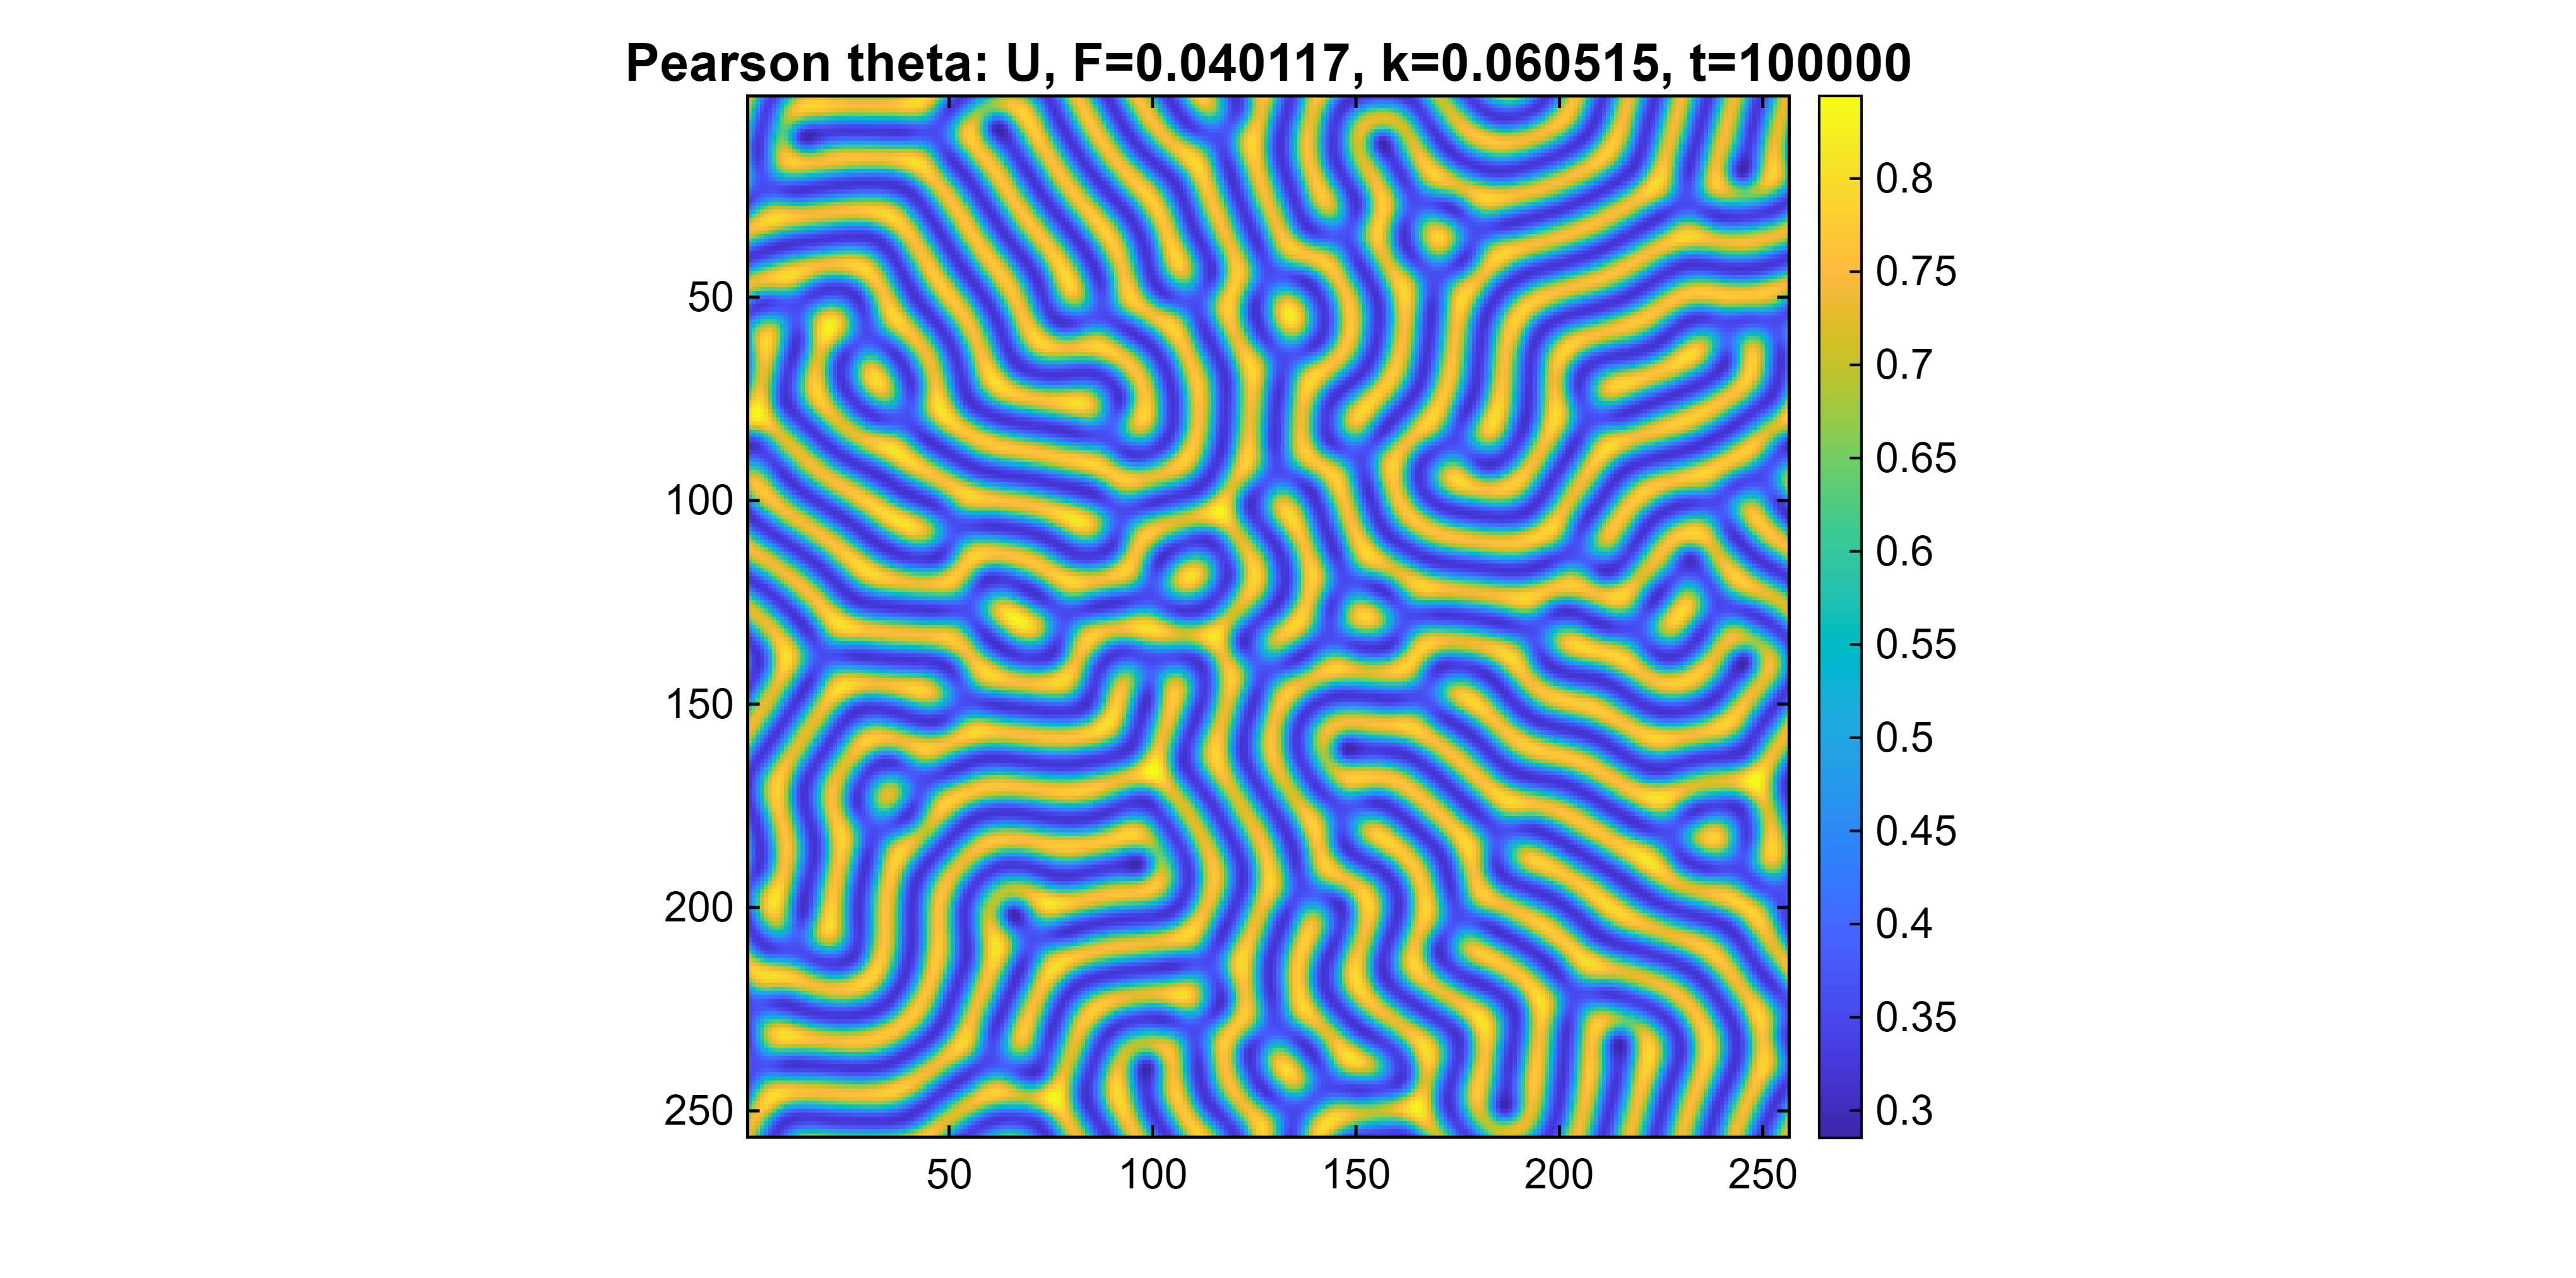
\includegraphics[width=0.95\textwidth]{figures/verification/pattern_sanity/theta_t100000_U.png}
\caption{Pearson \texttt{theta} case: representative \(U\)-field snapshot at \(t=100000\). The pattern is also labyrinth-like, but with a more intricate and locally curved stripe network than in the \texttt{kappa} case.}
\label{fig:pearson_theta_snapshot}
\end{figure}

\section{Verification summary}
\label{sec:verification_summary}

Overall, the verification results show that the implemented Gray--Scott solver behaves consistently with the expected numerical properties of the model and its discretization. The manufactured-solution operator test confirmed second-order spatial accuracy of the discrete Laplacian, while the time-step refinement study confirmed the expected first-order behavior of the explicit Euler method. The boundary-condition tests verified robust enforcement of Dirichlet and Neumann conditions, and the matrix--stencil comparison tests showed that the different diffusion implementations are equivalent both at the operator level and in full end-to-end simulations. In addition, the GUI and non-GUI comparison demonstrated that the graphical interface does not alter the numerical results. The supplementary checks further supported the structural correctness and internal consistency of the implementation. Taken together, these results provide strong verification evidence for the numerical core of the project, while the Pearson-type pattern study offers an additional validation-oriented sanity check at the application level.
\chapter{Computation Time Study}
TEXT PLACE HOLDER
\chapter{Benchmark and Solver Performance Study}

\section{Benchmark Goal and Design}

TEXT PLACEHOLDER.

\section{Benchmark Setup}

TEXT PLACEHOLDER.

\section{Compute-Only Runtime Comparison}

TEXT PLACEHOLDER.

\section{Live-Display Runtime Comparison}

TEXT PLACEHOLDER.

\section{Memory Footprint Comparison}

TEXT PLACEHOLDER.

\section{Scaling and Interpretation of Results}

TEXT PLACEHOLDER.

\section{Selection of the Recommended Default Solver}

TEXT PLACEHOLDER.
\chapter{Conclusion}

\section{Summary of Technical Achievements}

TEXT PLACEHOLDER.

\section{Main Numerical and Software Findings}

TEXT PLACEHOLDER.

\section{Final Takeaway}

TEXT PLACEHOLDER.

\bibliographystyle{unsrtnat}
\bibliography{BibTex}

\appendix
\chapter{Manual}

\section{Requirements, Project Layout, and Execution Modes}
\label{sec:manual_requirements}

The Gray--Scott project is designed to be executed directly from the root folder of the repository. The main requirement is a working MATLAB installation. In addition, MATLAB App Designer support is needed for the graphical user interface, because the GUI is stored as an \texttt{.mlapp} file. No external datasets, third-party libraries, or user-created input files are required for a standard simulation run. The program generates its own initial conditions internally and writes the produced outputs automatically to result folders.

For normal use, the most important files and folders are:

\begin{itemize}
    \item \texttt{run\_gui.m}: launcher for the graphical user interface.
    \item \texttt{run\_model\_class.m}: launcher for one standard non-GUI simulation run.
    \item \texttt{scripts/GrayScottController.mlapp}: App Designer GUI for interactive simulation and visualization.
    \item \texttt{src/}: numerical core of the project, including parameter handling, grid generation, diffusion operators, reaction term, time stepping, model class, and export utilities.
    \item \texttt{tests/}: verification, consistency, convergence, and benchmark scripts.
    \item \texttt{results/}: output folder created automatically during simulations, tests, GUI usage, and benchmark runs.
\end{itemize}

From the user point of view, the project provides four practical execution modes:

\begin{enumerate}
    \item \textbf{GUI mode:} interactive use through the App Designer interface for manual exploration of the model.
    \item \textbf{Non-GUI mode:} scripted execution through \texttt{run\_model\_class.m} for reproducible runs.
    \item \textbf{Test mode:} execution of the main verification suite through \texttt{tests/run\_all\_tests.m}.
    \item \textbf{Benchmark mode:} performance comparison of solver variants through \texttt{tests/benchmark\_solvers.m}.
\end{enumerate}

The project does not use external parameter files such as JSON, TXT, CSV, or XML files for standard runs. Instead, the simulation settings are stored in a MATLAB structure named \texttt{p}. In non-GUI mode, this structure is created directly in the launcher script. In GUI mode, the same parameter structure is managed internally through the interface controls. Thus, the effective input format of the program is a MATLAB parameter structure rather than a separate configuration file.

In the final project version, the stencil-based diffusion solver is the default choice for normal execution. The matrix-based and full-array variants remain available mainly for verification and benchmarking.

The following sections explain how to use the GUI, how to run the model without the GUI, how to execute the standard tests and the benchmark script, and where the generated outputs are stored.

\section{How to Run the GUI}
\label{sec:manual_gui}

The graphical user interface is the most convenient execution mode for interactive exploration of the Gray--Scott model. To start it, open the project root folder in MATLAB and run

\begin{verbatim}
run_gui
\end{verbatim}

This command adds the required source folders to the MATLAB path and launches the App Designer application \texttt{GrayScottController}. The GUI is not a separate implementation of the model. It uses the same numerical core as the scripted workflow, but provides an interactive front end for changing settings and visualizing the results.

At startup, the GUI creates a default Gray--Scott model automatically and opens a separate plot window. In the final project version, the GUI uses the stencil-based diffusion solver as its normal execution mode.

The main user-controlled settings in the GUI are:

\begin{itemize}
    \item \textbf{Run control:} \texttt{Run}, \texttt{Pause}, \texttt{Reset}, and \texttt{Restart}.
    \item \textbf{Reaction parameters:} the sliders for \texttt{F} and \texttt{k}.
    \item \textbf{Displayed field:} selection of the plotted concentration field \texttt{U} or \texttt{V}.
    \item \textbf{Boundary conditions:} \texttt{Periodic}, \texttt{Neumann}, or \texttt{Dirichlet}.
    \item \textbf{Visual options:} colormap and plotting appearance.
    \item \textbf{Recording options:} video frame rate and video format.
    \item \textbf{Pattern presets:} predefined \texttt{F}-\texttt{k} combinations for characteristic pattern regimes.
\end{itemize}

The diffusion coefficients \texttt{D\_u} and \texttt{D\_v} are shown in the interface for transparency, but in the final GUI they are read-only. Therefore, the GUI is mainly intended for interactive study of pattern formation through the parameters \texttt{F} and \texttt{k}, while more detailed changes are better handled in the scripted non-GUI workflow.

A typical GUI workflow is as follows:

\begin{enumerate}
    \item Start the application with \texttt{run\_gui}.
    \item Select the field to display, usually \texttt{V}, because it shows the pattern structure clearly.
    \item Adjust \texttt{F} and \texttt{k} manually or choose a preset from the menu.
    \item Select the desired boundary-condition type.
    \item Press \texttt{Run} to start the simulation and \texttt{Pause} to stop it temporarily.
    \item Use \texttt{Restart} if the simulation should begin again with the current \texttt{F} and \texttt{k} values.
    \item Use \texttt{Reset} if the GUI should return to its original default values and rebuild the initial state.
\end{enumerate}

The difference between \texttt{Reset} and \texttt{Restart} is important. \texttt{Restart} keeps the currently selected reaction parameters and rebuilds the model from the beginning using those values. \texttt{Reset}, in contrast, restores the original GUI defaults and then rebuilds the model. This allows the user either to repeat the current configuration or to return quickly to the startup configuration.

The GUI also supports model storage through the \texttt{File} menu. The entry \texttt{Save model} stores the current model object as a MATLAB \texttt{.mat} file, and \texttt{Load model} reloads such a saved model. Video recording can also be activated directly in the GUI. When recording is enabled, the application writes a video file automatically to the \texttt{results/} folder.

As a simple example, suppose that the user wants to inspect a spot-forming regime visually. A practical procedure is to start the GUI, select the \texttt{V} field, choose an appropriate spot-like preset from the menu, and press \texttt{Run}. If the generated pattern is interesting, recording can be activated before the next run so that the temporal evolution is saved automatically. If the same pattern should then be compared under a different boundary condition, the boundary-condition type can be changed and the model can be started again from the initial state.

The GUI is therefore best suited for exploratory work, visual comparison of parameter choices, video recording, and demonstration of the model during presentations. For reproducible scripted runs with explicit parameter editing, the non-GUI workflow is more appropriate.

\section{How to Run the Model Without the GUI}
\label{sec:manual_nongui}

The non-GUI workflow is intended for reproducible scripted simulations. It is the most suitable execution mode when parameter values should be documented explicitly, when a run should be repeated under controlled conditions, or when output files should be generated in an organized run folder.

To execute one standard simulation without the graphical user interface, open the root folder of the project in MATLAB and run

\begin{verbatim}
run_model_class
\end{verbatim}

The script creates the parameter structure \texttt{p}, normalizes it, builds the computational grid, initializes the \texttt{GrayScottModel} object, performs the time-stepping loop, optionally updates a live figure, optionally exports PNG snapshots, and finally stores the last simulation state.

\subsection*{Basic workflow}

The normal workflow of \texttt{run\_model\_class.m} is:

\begin{enumerate}
    \item add the \texttt{src/} folder to the MATLAB path,
    \item create a default parameter structure \texttt{p},
    \item select the diffusion mode,
    \item call \texttt{finalizeParams(p)} to normalize and validate the settings,
    \item create a timestamp-based output folder inside \texttt{results/},
    \item run the simulation,
    \item save the main outputs of the run.
\end{enumerate}

In the final project version, the script uses the stencil solver as the default solver. Thus, a normal call of \texttt{run\_model\_class} already starts from the recommended standard execution mode.

\subsection*{Parameter format}

The non-GUI launcher does not read a separate external parameter file. Instead, all simulation inputs are defined directly in MATLAB through the structure \texttt{p}. The most important fields are:

\begin{itemize}
    \item \texttt{Du}, \texttt{Dv}, \texttt{F}, \texttt{k}: Gray--Scott model parameters,
    \item \texttt{Nx}, \texttt{Ny}, \texttt{Lx}, \texttt{Ly}: grid and domain parameters,
    \item \texttt{dt}, \texttt{T}: time-step size and final time,
    \item \texttt{seed}, \texttt{icType}, \texttt{icPerturb}: initial-condition settings,
    \item \texttt{diffusionMode}: solver selection,
    \item \texttt{plotField}, \texttt{plotEvery}, \texttt{savePngEvery}: output control,
    \item \texttt{BC}: per-side boundary-condition structure.
\end{itemize}

Some of these fields use fixed keywords that must be written exactly:

\begin{itemize}
    \item \texttt{diffusionMode}: \texttt{"matrix"}, \texttt{"stencil"}, or \texttt{"full"},
    \item \texttt{plotField}: \texttt{"u"} or \texttt{"v"},
    \item \texttt{p.BC.<side>.type}: \texttt{"periodic"}, \texttt{"dirichlet"}, or \texttt{"neumann"},
    \item \texttt{defaultParams(...)} presets: \texttt{"baseline"} or \texttt{"pearson"}.
\end{itemize}

The call to \texttt{finalizeParams(p)} is important because it checks and normalizes these entries before the simulation starts. If a keyword is written incorrectly, the script stops with an error instead of running with an inconsistent setup.

\subsection*{Important execution rule}

The script computes the number of time steps as \texttt{Nt = T / dt}. Therefore, the chosen values of \texttt{T} and \texttt{dt} must be compatible such that \texttt{T/dt} is an integer. Otherwise the script stops with an error. When parameters are modified manually, this condition should always be checked.

\subsection*{Simple examples}

\textbf{Example 1: standard run.}  
For a default run with the standard stencil solver, no manual changes are needed. Open the project root folder and execute

\begin{verbatim}
run_model_class
\end{verbatim}

This uses the default parameter structure, runs one simulation, and writes the outputs automatically into a newly created subfolder of \texttt{results/}.

\medskip

\textbf{Example 2: change the preset and output settings.}  
A user may want to start from the Pearson-style preset, visualize the \texttt{u}-field, and export images less frequently. In that case, the beginning of \texttt{run\_model\_class.m} can be edited as follows:

\begin{verbatim}
p = defaultParams("pearson");
p.diffusionMode = "stencil";
p.plotField = "u";
p.plotEvery = 50;
p.savePngEvery = 100;
p = finalizeParams(p);
\end{verbatim}

After saving the file, run

\begin{verbatim}
run_model_class
\end{verbatim}

The simulation will then use the Pearson-type parameter set and export snapshots of the selected field according to the specified output cadence.

\medskip

\textbf{Example 3: modify one model parameter and the boundary condition.}  
To compare the influence of a different feed rate and a different boundary-condition type, the parameter block can be edited, for example, to

\begin{verbatim}
p = defaultParams();
p.diffusionMode = "stencil";
p.F = 0.022;
p.k = 0.051;

p.BC.left.type   = "neumann";
p.BC.right.type  = "neumann";
p.BC.bottom.type = "neumann";
p.BC.top.type    = "neumann";

p = finalizeParams(p);
\end{verbatim}

This produces a run with modified reaction parameters and homogeneous Neumann conditions on all four boundaries.

\subsection*{Plotting and PNG export}

The non-GUI script distinguishes between live plotting and image export:

\begin{itemize}
    \item \texttt{plotEvery} controls how often the MATLAB figure is updated during the run,
    \item \texttt{savePngEvery} controls how often PNG files are written to disk.
\end{itemize}

A value of \texttt{0} disables the corresponding feature. For example, setting

\begin{verbatim}
p.plotEvery = 0;
p.savePngEvery = 0;
\end{verbatim}

disables intermediate live plotting and intermediate PNG export. The script still saves the final state and exports one final snapshot at the end of the run.

\section{How to Run the Tests}
\label{sec:manual_tests}

The project contains a structured verification folder for automated checks of the numerical implementation. These tests are intended to confirm that the solver behaves correctly with respect to operator properties, boundary-condition handling, manufactured-solution verification, time-step behavior, and agreement between different diffusion implementations.

In the final project version, the standard test entry point is

\begin{verbatim}
tests/run_all_tests
\end{verbatim}

If MATLAB is already opened inside the \texttt{tests/} folder, the same suite can also be started with

\begin{verbatim}
run_all_tests
\end{verbatim}

The script adds the required project paths automatically, executes the selected verification tests one after another, prints a pass/fail summary in the MATLAB command window, and stores a summary file under \texttt{results/tests/}.

\subsection*{Standard verification suite}

The standard test runner contains the important fast-to-moderate checks that should be executed routinely. In the final repository, these are:

\begin{itemize}
    \item \texttt{test\_laplacian\_constant}: checks that the Laplacian behaves correctly for a constant field.
    \item \texttt{test\_laplacian\_symmetry}: checks the expected symmetry property of the discrete operator.
    \item \texttt{test\_boundary\_conditions}: verifies boundary-condition handling.
    \item \texttt{test\_timestep\_halving\_smoke}: short smoke test for time-step refinement behavior.
    \item \texttt{test\_mms\_endtoend}: manufactured-solution verification of the full solver workflow.
    \item \texttt{test\_mms\_operator\_convergence}: convergence check for the discrete operator.
    \item \texttt{test\_timestep\_convergence}: verification of the expected time-step behavior.
    \item \texttt{test\_laplacian\_stencil\_equivalence}: agreement check between stencil and matrix-style Laplacian application.
    \item \texttt{test\_matrix\_stencil\_endtoend\_equivalence}: end-to-end comparison between matrix and stencil solver paths.
\end{itemize}

This curated set is the recommended standard verification procedure for routine use because it covers the essential numerical properties without including the longest validation scripts.

\subsection*{Long or special tests to run separately}

Not every script in the \texttt{tests/} folder belongs to the standard routine suite. Some checks are intentionally kept separate because they are slower, more qualitative, or intended for special validation tasks.

\textbf{1. Pearson pattern sanity test}

The script

\begin{verbatim}
tests/test_pattern_sanity_pearson
\end{verbatim}

is a long qualitative validation run based on Pearson-style cases. It is intended for visual sanity checking of the produced patterns rather than for fast routine testing.

\medskip

\textbf{2. Grid-refinement study}

The script

\begin{verbatim}
tests/test_grayscott_grid_refinement
\end{verbatim}

performs a dedicated grid-refinement study. Because it is more expensive than the routine checks and is used for a specific numerical study, it is better treated as a standalone verification script.

\medskip

\textbf{3. GUI versus non-GUI consistency check}

The folder \texttt{tests/gui\_consistency/} contains a separate workflow to verify that the GUI reproduces the same numerical results as the non-GUI execution path. This check is not part of \texttt{run\_all\_tests}, because it requires a dedicated comparison workflow. The recommended procedure is:

\begin{verbatim}
ref = run_nongui_reference_dump();
gui = run_gui_consistency_dump();
T   = compare_gui_nongui(ref.refFile, gui.guiFile);
\end{verbatim}

This workflow generates reference dumps, compares intermediate and final states, and saves comparison outputs for later inspection.

For ordinary development and routine verification, the standard call to \texttt{run\_all\_tests} is sufficient and recommended. The standalone scripts should be used only when their specific purpose is needed.

\section{How to Run the Benchmarks}
\label{sec:manual_benchmarks}

The benchmark scripts are intended for systematic performance comparison of the available diffusion implementations. In the final project version, the main benchmark entry point is the MATLAB function \texttt{benchmark\_solvers()}, which compares the sparse-matrix solver, the stencil-based solver, and the dense/full solver under a fixed benchmark protocol. The benchmark is not a verification test in the strict sense; instead, it measures runtime and memory-related quantities for the different implementations under controlled conditions.

To run the benchmark from MATLAB, a practical procedure from the project root folder is

\begin{verbatim}
addpath(genpath(fullfile(pwd,'tests')));
benchmark_solvers
\end{verbatim}

The benchmark script itself adds the required source folders automatically, so the main purpose of the \texttt{addpath} command above is to make the benchmark function callable from the project root. After the run finishes, MATLAB writes the results into a new timestamp-based benchmark folder under \texttt{results/}.

\subsection*{What the benchmark measures}

The benchmark compares three diffusion realizations:

\begin{itemize}
    \item \texttt{matrix}: sparse Laplacian matrix multiplication,
    \item \texttt{stencil}: matrix-free stencil diffusion,
    \item \texttt{full}: dense/full Laplacian matrix multiplication.
\end{itemize}

It evaluates these solvers in two timing modes:

\begin{itemize}
    \item \texttt{compute\_off}: solver runtime without live visualization,
    \item \texttt{render\_on}: solver runtime with live display updates.
\end{itemize}

The timed region contains only the stepping loop. Grid construction, operator setup, initial-condition preparation, and warm-up steps are excluded from the timed interval. This makes the benchmark suitable for comparing the solver cost itself rather than the total startup overhead.

\subsection*{Default benchmark setup}

In the final repository, the benchmark uses the following default configuration:

\begin{itemize}
    \item grid sizes: \texttt{32x32}, \texttt{64x64}, \texttt{128x128}, \texttt{256x256}, and \texttt{512x512},
    \item dense/full solver only on \texttt{32x32}, \texttt{64x64}, and \texttt{128x128},
    \item warm-up steps: \texttt{50},
    \item timed steps: \texttt{500},
    \item repetitions per case: \texttt{7},
    \item random seed: \texttt{1},
    \item live-display update interval in render mode: every \texttt{10} steps.
\end{itemize}

These settings are already encoded in the final benchmark script and normally do not need to be changed for routine use.

\subsection*{Simple benchmark example}

A standard benchmark run consists of the following MATLAB commands:

\begin{verbatim}
addpath(genpath(fullfile(pwd,'tests')));
benchmark_solvers
\end{verbatim}

After the computation finishes, inspect the newest benchmark folder inside \texttt{results/}. It contains the main benchmark data files, including a MATLAB data file and a CSV table for later analysis.

\subsection*{Interpretation note}

The benchmark is designed specifically to compare diffusion implementations under a common numerical setup. The diffusion operators use periodic connectivity internally, while physical boundary conditions such as Dirichlet or Neumann are enforced after each time step rather than being part of the benchmarked operator itself. Therefore, the benchmark should be interpreted as a solver-performance study and not as a comparison of different physical boundary-condition models.

\section{Output Folders and Generated Files}
\label{sec:manual_outputs}

The project writes its generated data automatically into output folders, so the user normally does not need to create result directories manually. Most outputs are stored under the folder \texttt{results/}. The exact files depend on the selected execution mode.

\subsection*{Outputs of a non-GUI simulation run}

When \texttt{run\_model\_class} is executed, the script creates a new timestamp-based subfolder inside \texttt{results/}. Its structure has the form

\begin{verbatim}
results/<timestamp>_<caseName>/
\end{verbatim}

This folder collects the outputs of exactly one scripted simulation run. The most important generated files are:

\begin{itemize}
    \item \texttt{meta.mat}: MATLAB data file containing metadata of the run, including the parameter structure.
    \item \texttt{log.txt}: text summary of the most important run settings.
    \item PNG image files: exported snapshots of the selected field during the run and at the final state.
    \item \texttt{final\_state.mat}: MATLAB file containing the final numerical state of the simulation.
\end{itemize}

These files make the non-GUI workflow reproducible and suitable for later inspection.

\subsection*{Outputs of the GUI}

The GUI also writes files automatically into the \texttt{results/} folder when save or recording operations are used. In practical use, the most relevant GUI-generated outputs are:

\begin{itemize}
    \item saved model files in MATLAB \texttt{.mat} format,
    \item recorded video files of simulation runs.
\end{itemize}

The saved model files are useful when a simulation state should be reopened later from the GUI. The video files are produced when recording is enabled in the interface.

\subsection*{Outputs of the standard test suite}

The standard verification suite started by

\begin{verbatim}
tests/run_all_tests
\end{verbatim}

stores its collected summary in

\begin{verbatim}
results/tests/results_summary.mat
\end{verbatim}

This file contains the returned result structures of the executed routine tests. The command window output during the test run provides the immediate pass/fail feedback, while \texttt{results\_summary.mat} stores the structured data for later use.

Longer standalone validation scripts may generate their own outputs depending on the specific workflow. For example, dedicated GUI consistency checks create separate comparison data for inspection.

\subsection*{Outputs of the benchmark workflow}

The benchmark function creates a separate timestamp-based output folder of the form

\begin{verbatim}
results/benchmarks_<timestamp>/
\end{verbatim}

Inside this folder, the main generated files are:

\begin{itemize}
    \item \texttt{benchmark\_results.mat}: raw MATLAB benchmark data,
    \item \texttt{benchmark\_table.csv}: tabulated benchmark summary.
\end{itemize}

The MATLAB file is useful for later detailed analysis in MATLAB, while the CSV file is convenient for inspection, table generation, or further processing.

\subsection*{Practical interpretation of file formats}

The generated file formats in the project have the following practical roles:

\begin{itemize}
    \item \texttt{.mat}: MATLAB-native storage of states, models, metadata, and structured results.
    \item \texttt{.txt}: human-readable summaries such as run logs.
    \item \texttt{.png}: image export for simulation snapshots.
    \item video files: recorded GUI animations for presentation and visual inspection.
    \item \texttt{.csv}: tabulated benchmark data for easy comparison and export.
\end{itemize}

Thus, the project does not require external input data files for normal execution, but it does produce several well-defined output formats for analysis, visualization, and documentation.
\input{appendices/B_git_log}

\end{document}